\chapter{Reconstrucci\'on de eventos y selecci\'on de candidatos}
\label{ch:selAuger}

En este capítulo se describe la metodología aplicada para elegir el criterio de selección en las tres búsquedas.
En primer lugar se definen cortes de calidad que eliminan estaciones o incluso eventos espúreos, con el fin de lograr una reconstrucción confiable.
Una vez logrado, se utilizan variables topológicas y temporales para seleccionar eventos inclinados, y luego  se agrega información de las trazas para discriminar las lluvias jóvenes.

\section{Criterios de calidad}

	Al inicio de la cadena de procesamiento se cuenta con un conjunto de eventos que cumplen el criterio de trigger T3.
	De este grupo, se eliminan en primer lugar los datos que se hayan tomado en períodos en los que el detector se haya comportado de manera inestable\cite{pmtsAuger}.
	Luego, se aplica a cada evento una serie de procedimientos que se mencionan a continuación:
	\begin{itemize}
	 \item Selección de tubos fotomultiplicadores (PMT's)
	 \item Selección de estaciones
	 \item Reconstrucción preeliminar
	 \item Cortes adicionales
	\end{itemize}
	
	\subsection{Selección de tubos fotomultiplicadores}
	
	La búsqueda de neutrinos consiste en encontrar eventos extremadamente raros en el detector, por lo que en caso de aparecer algun candidato, es de extrema importancia que todas sus estaciones posean PMT's que funcionen correctamente.
	En particular es vital descartar los PMT's que posean patologías que alarguen la señal en el tiempo, ya que, como se verá en la sección \ref{sc:selNu}, la selección de lluvias jóvenes depende fuertemente de este factor.
	
	Hay varios cortes que se utilizan para descartar PMT's. 
	Estos pueden ser separados en dos grupos, que se describen a continuación.
	
		\subsubsection{Criterios basados en la integral de la señal}
		
		Este conjunto de cortes es el resultado de estudios llevados a cabo por el grupo de monitoreo del observatorio~\cite{pmtsAuger}. 
		A partir de ellos se provee una lista de PMT's inestables día a día.
		Los parámetros que se utilizan para definir esta clasificación son las líneas de base del ánodo, del dínodo y la llamada relación dínodo-ánodo (RDA).
		En el caso de las líneas de base se impone un l\'imite a las fluctuaciones, mediante un corte en su RMS de los valores diarios, mientras que para la RDA se limita adem\'as su valor máximo y mínimo.
		
		La figura \ref{fig:event1634332} muestra un ejemplo en el que el PMT número 3 es descartado debido a que posee una relación dínodo/ánodo mayor al permitido, mientras que las otras dos estaciones muestran valores normales.
		
		 \begin{figure}[h!]
			\begin{center}
			$
			\begin{array}{cc}
			\text{\'Anodo} &\text{D\'inodo} \\
			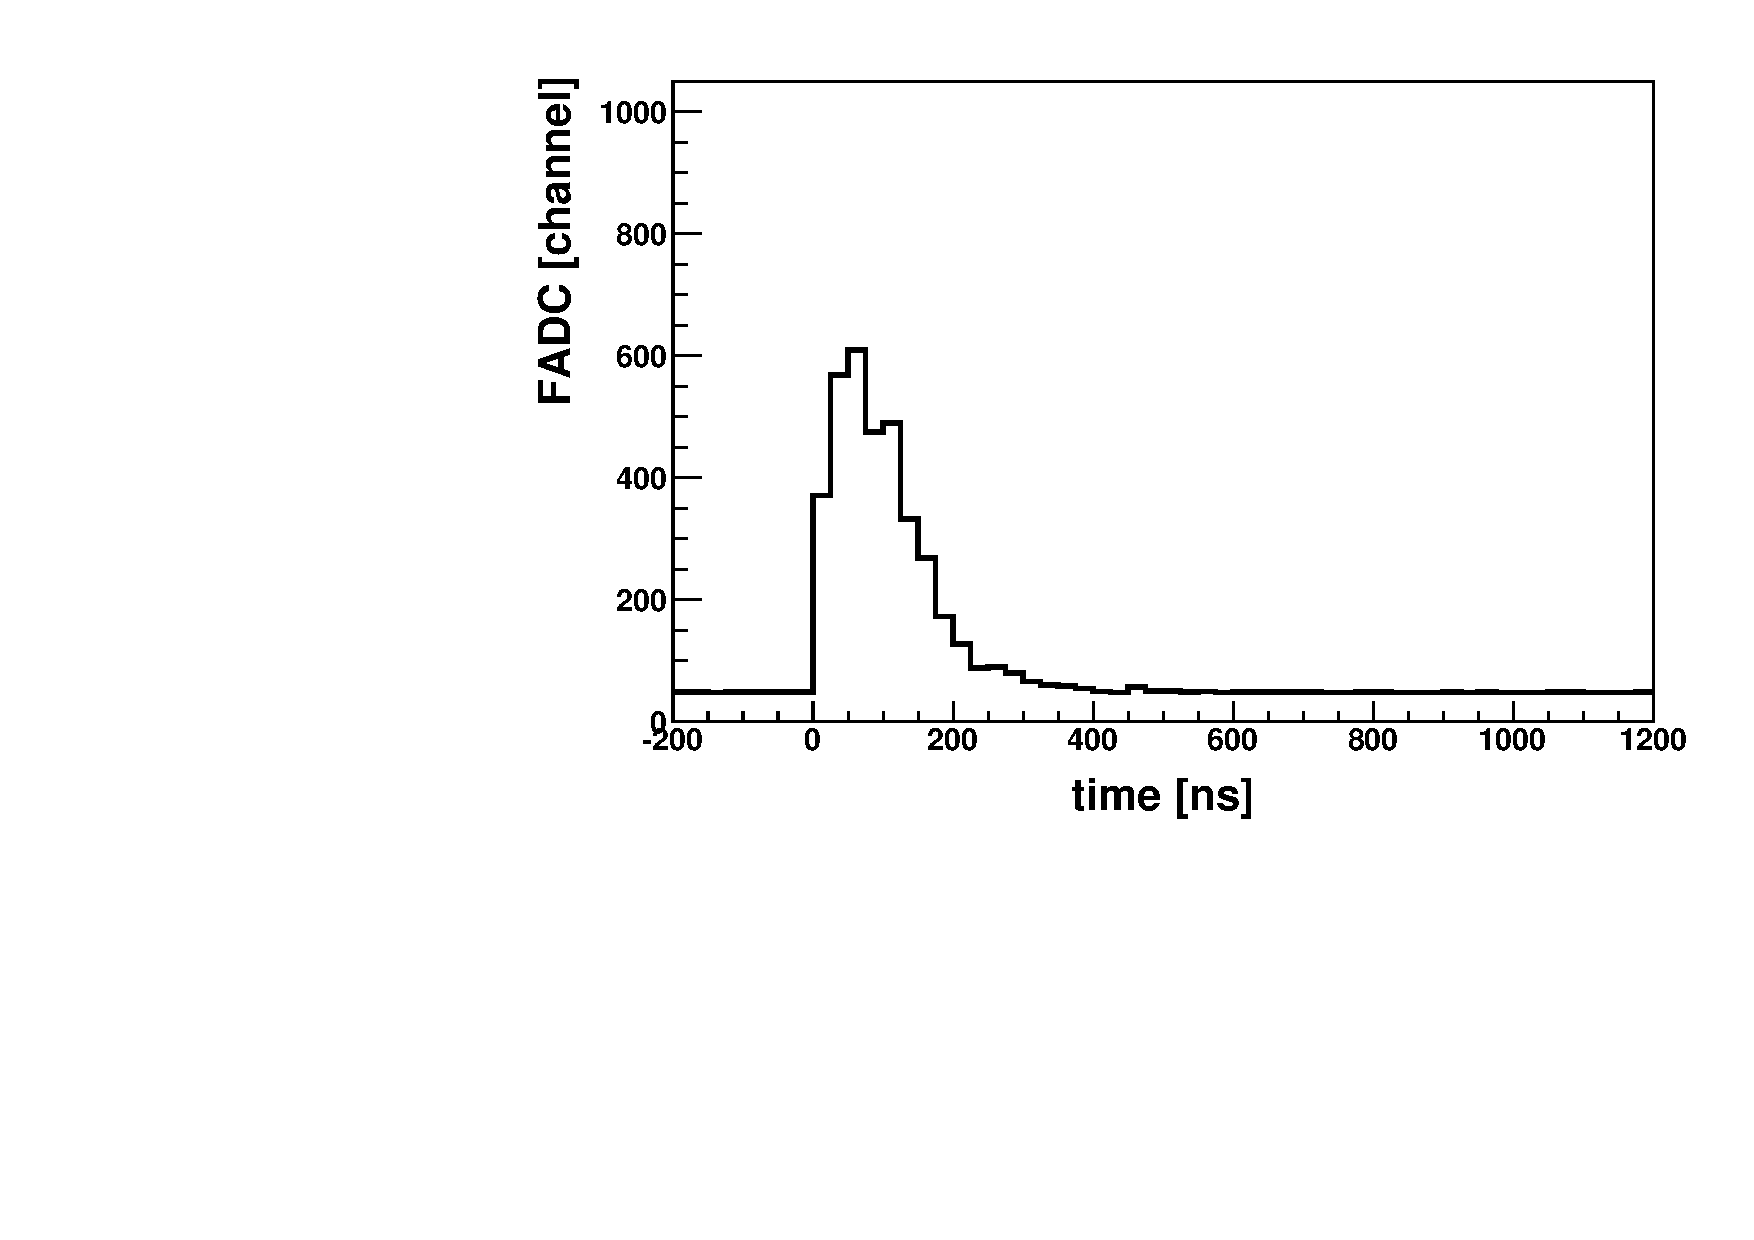
\includegraphics[width=0.47\textwidth]{fig/seleccionAuger/ev1634332_pmt1_anode.pdf} & 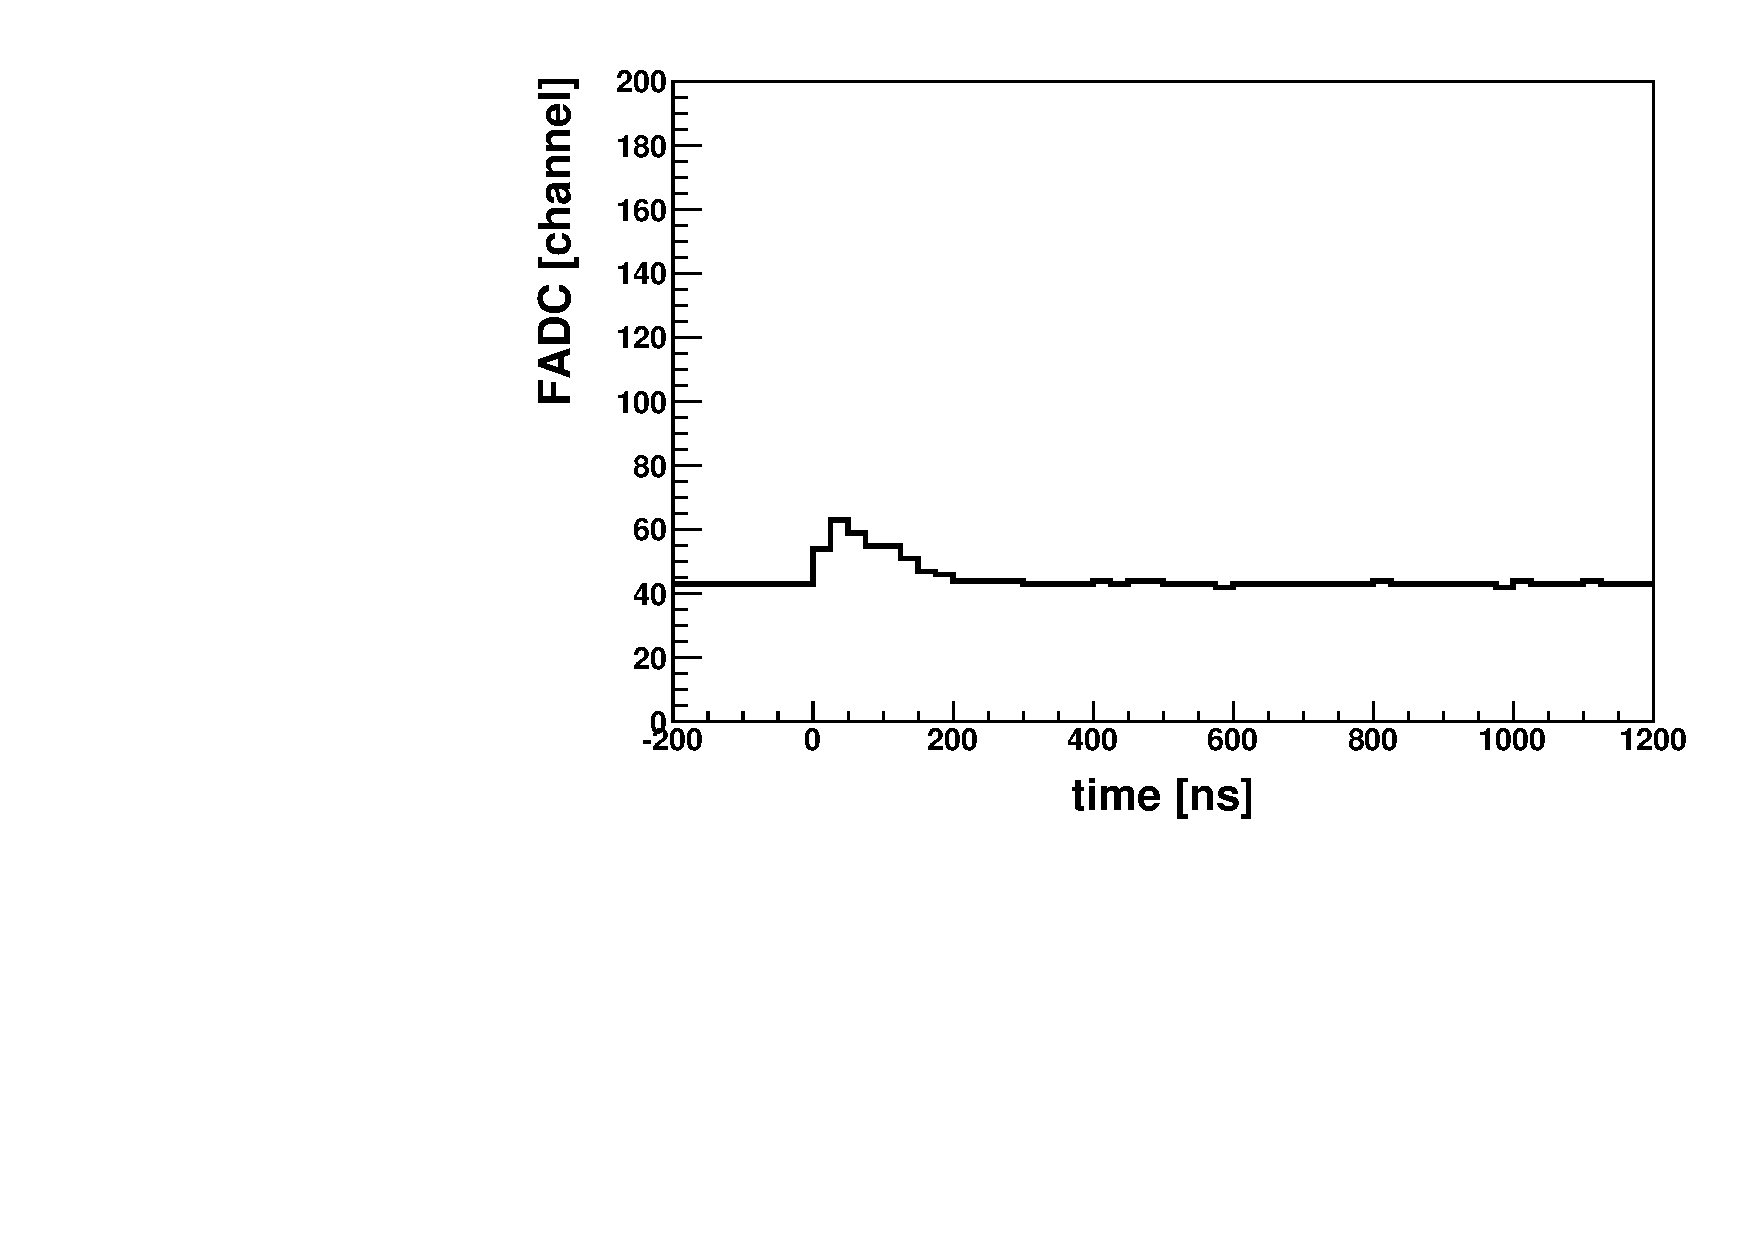
\includegraphics[width=0.47\textwidth]{fig/seleccionAuger/ev1634332_pmt1_dynode.pdf}\\
			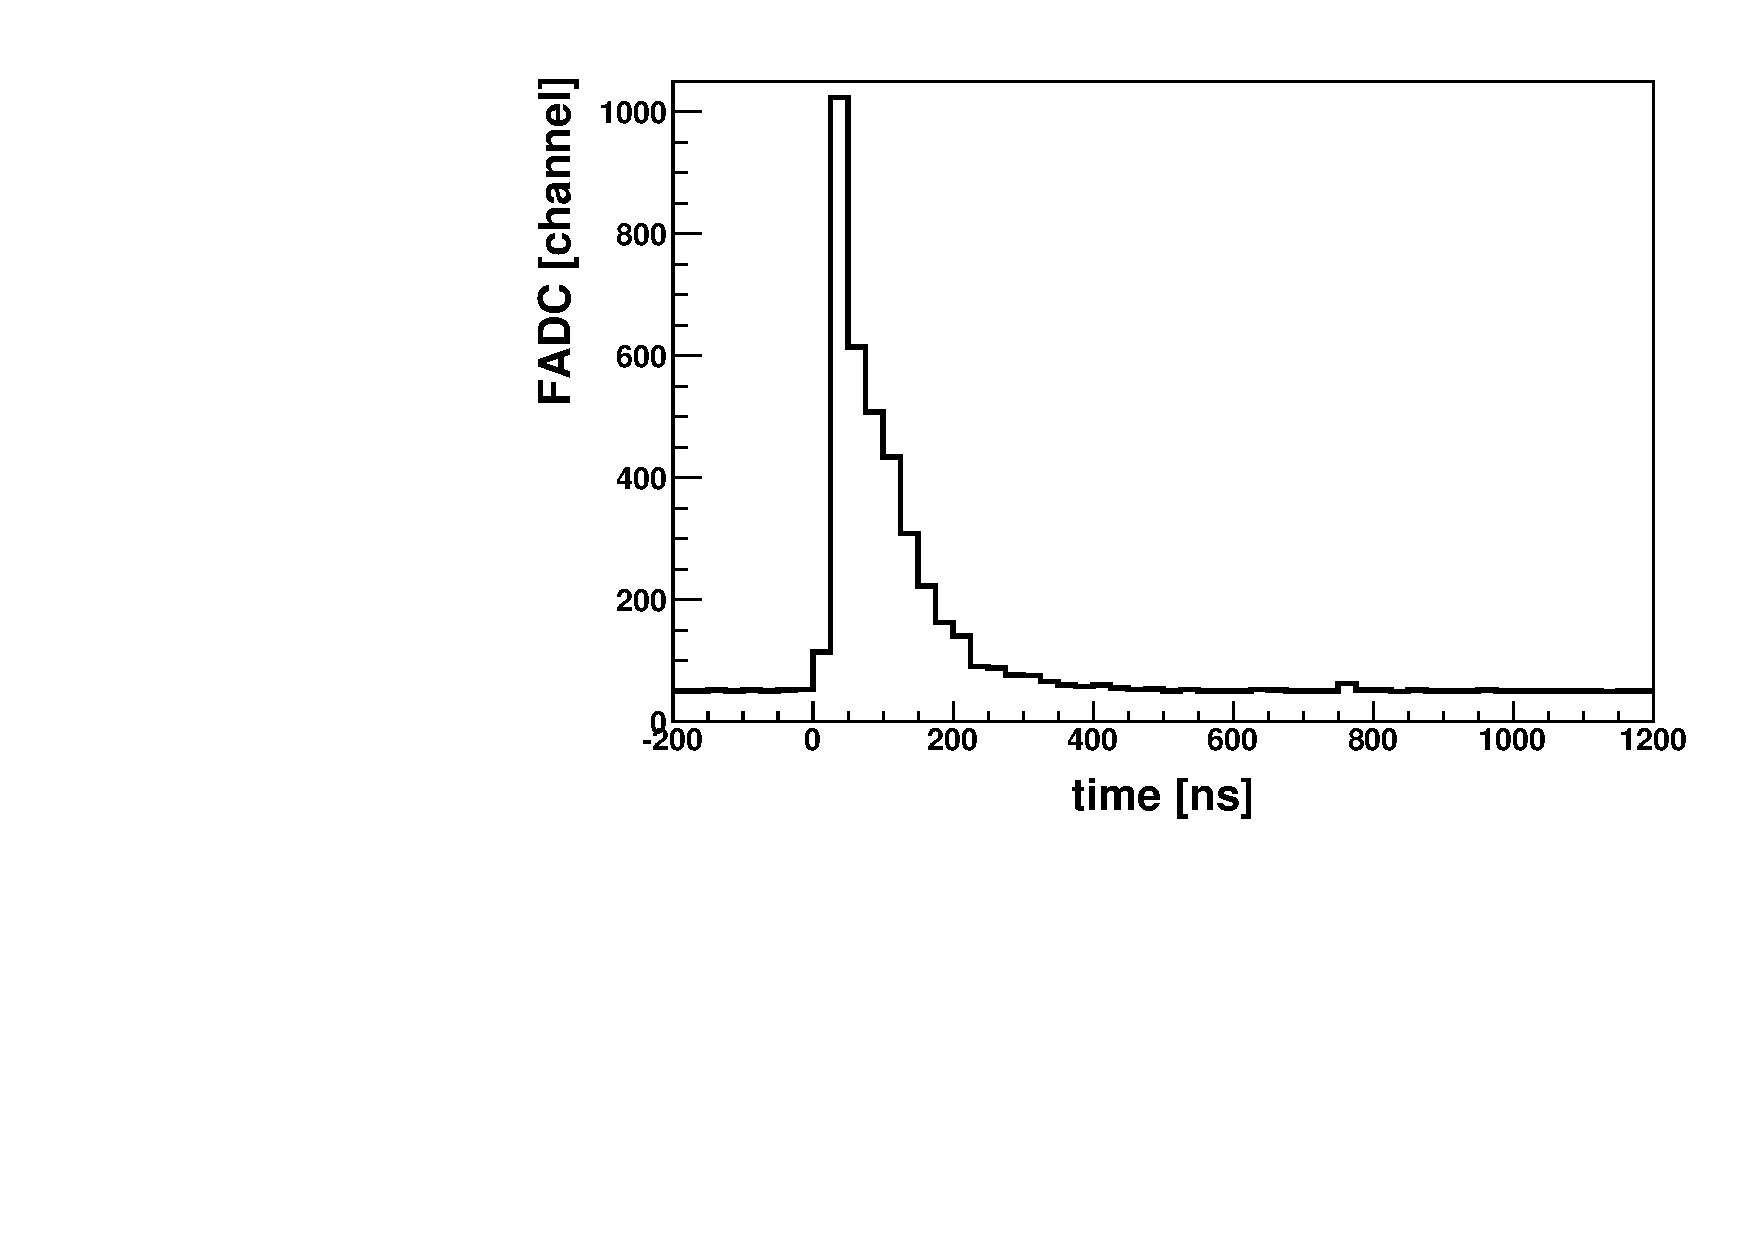
\includegraphics[width=0.47\textwidth]{fig/seleccionAuger/ev1634332_pmt2_anode.pdf} & 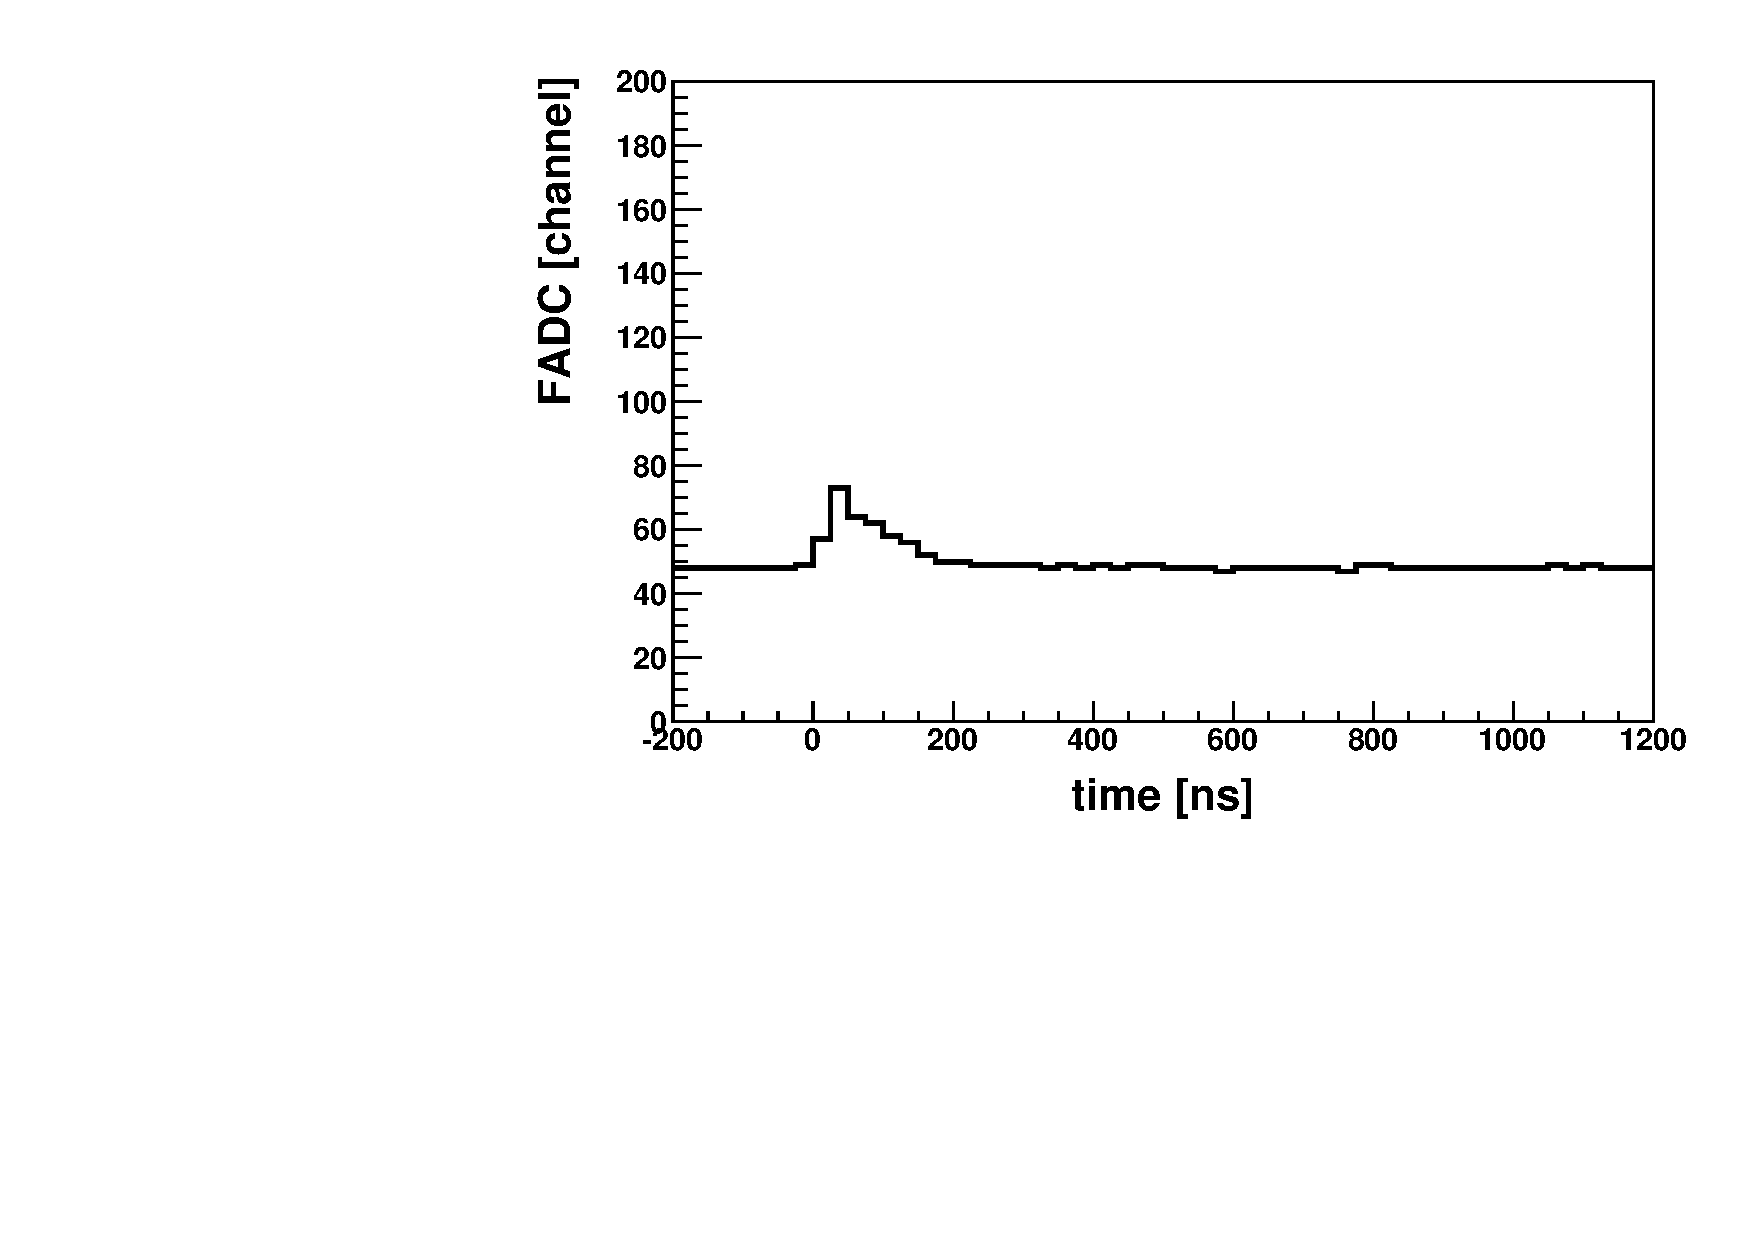
\includegraphics[width=0.47\textwidth]{fig/seleccionAuger/ev1634332_pmt2_dynode.pdf}\\
			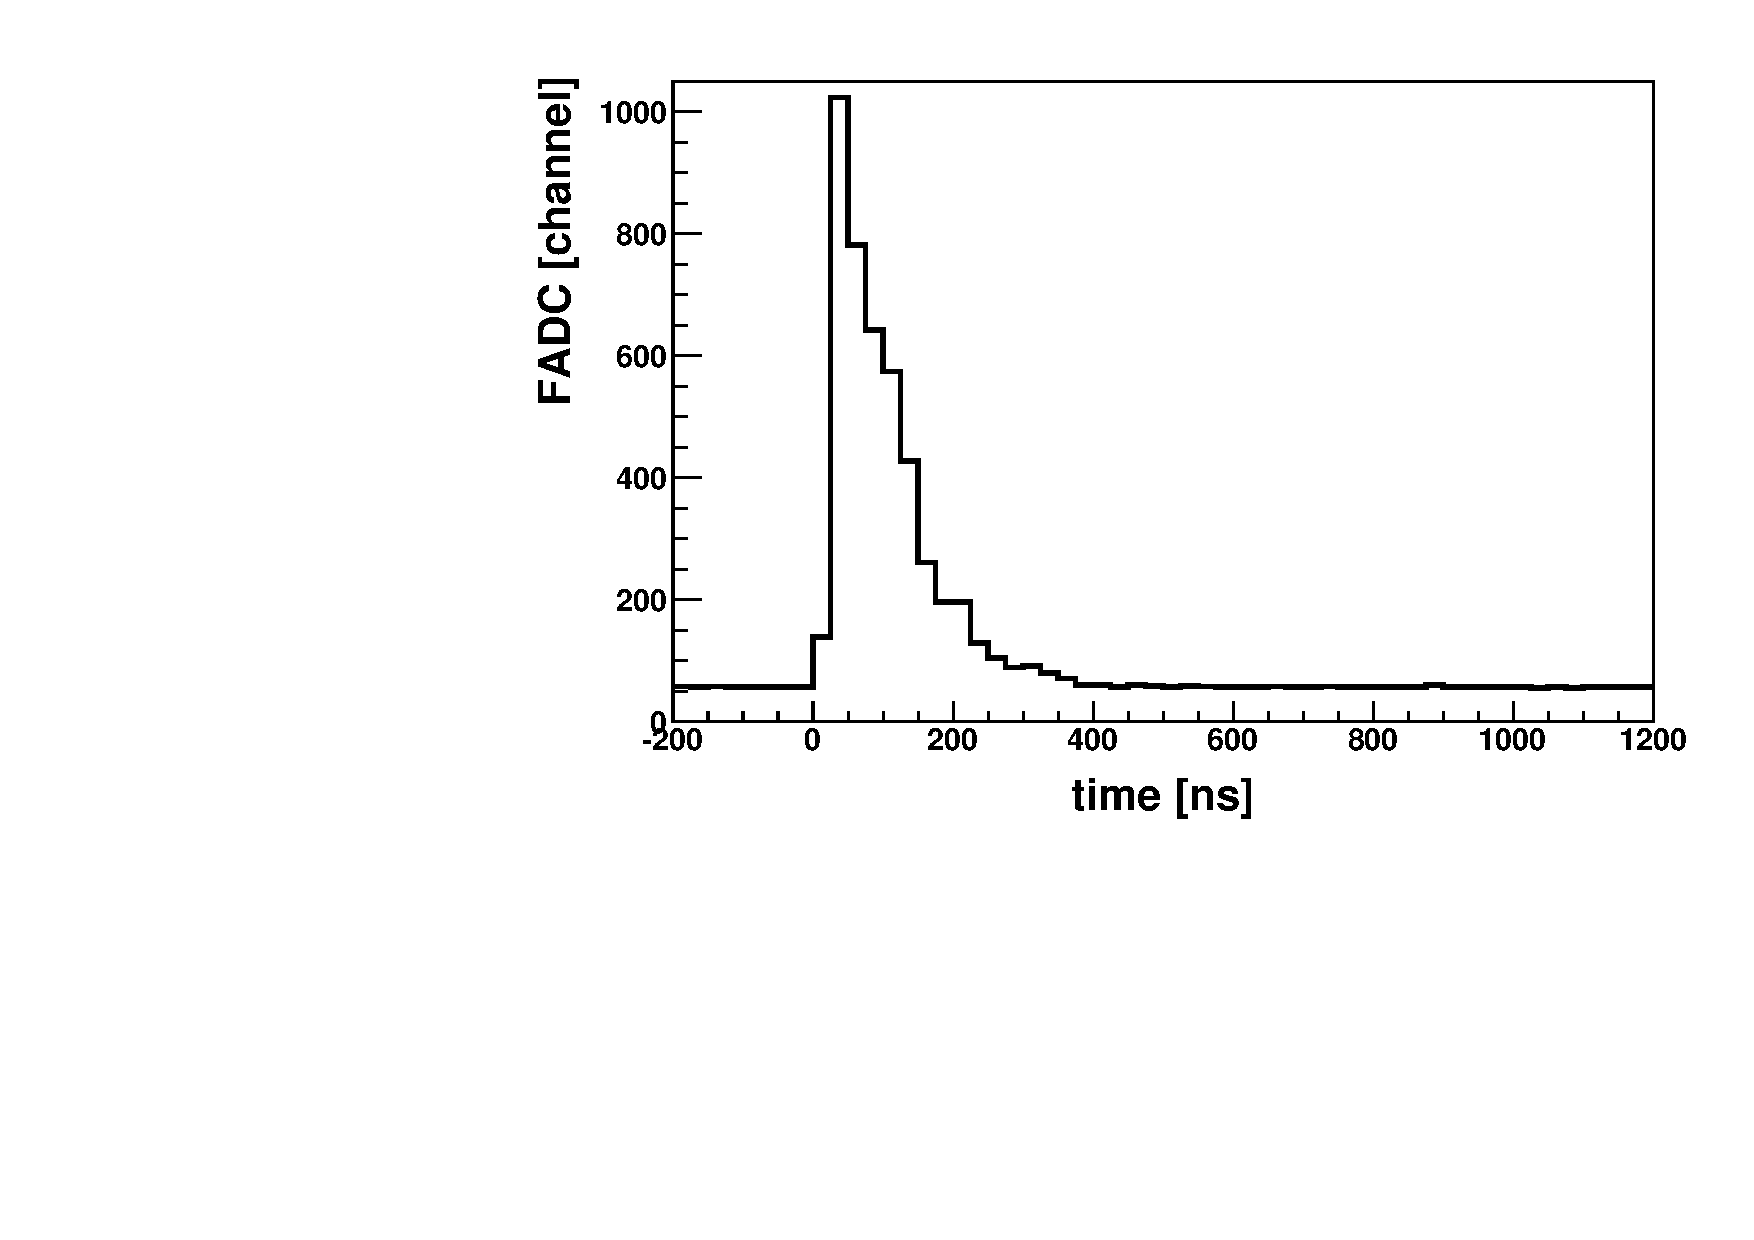
\includegraphics[width=0.47\textwidth]{fig/seleccionAuger/ev1634332_pmt3_anode.pdf} & 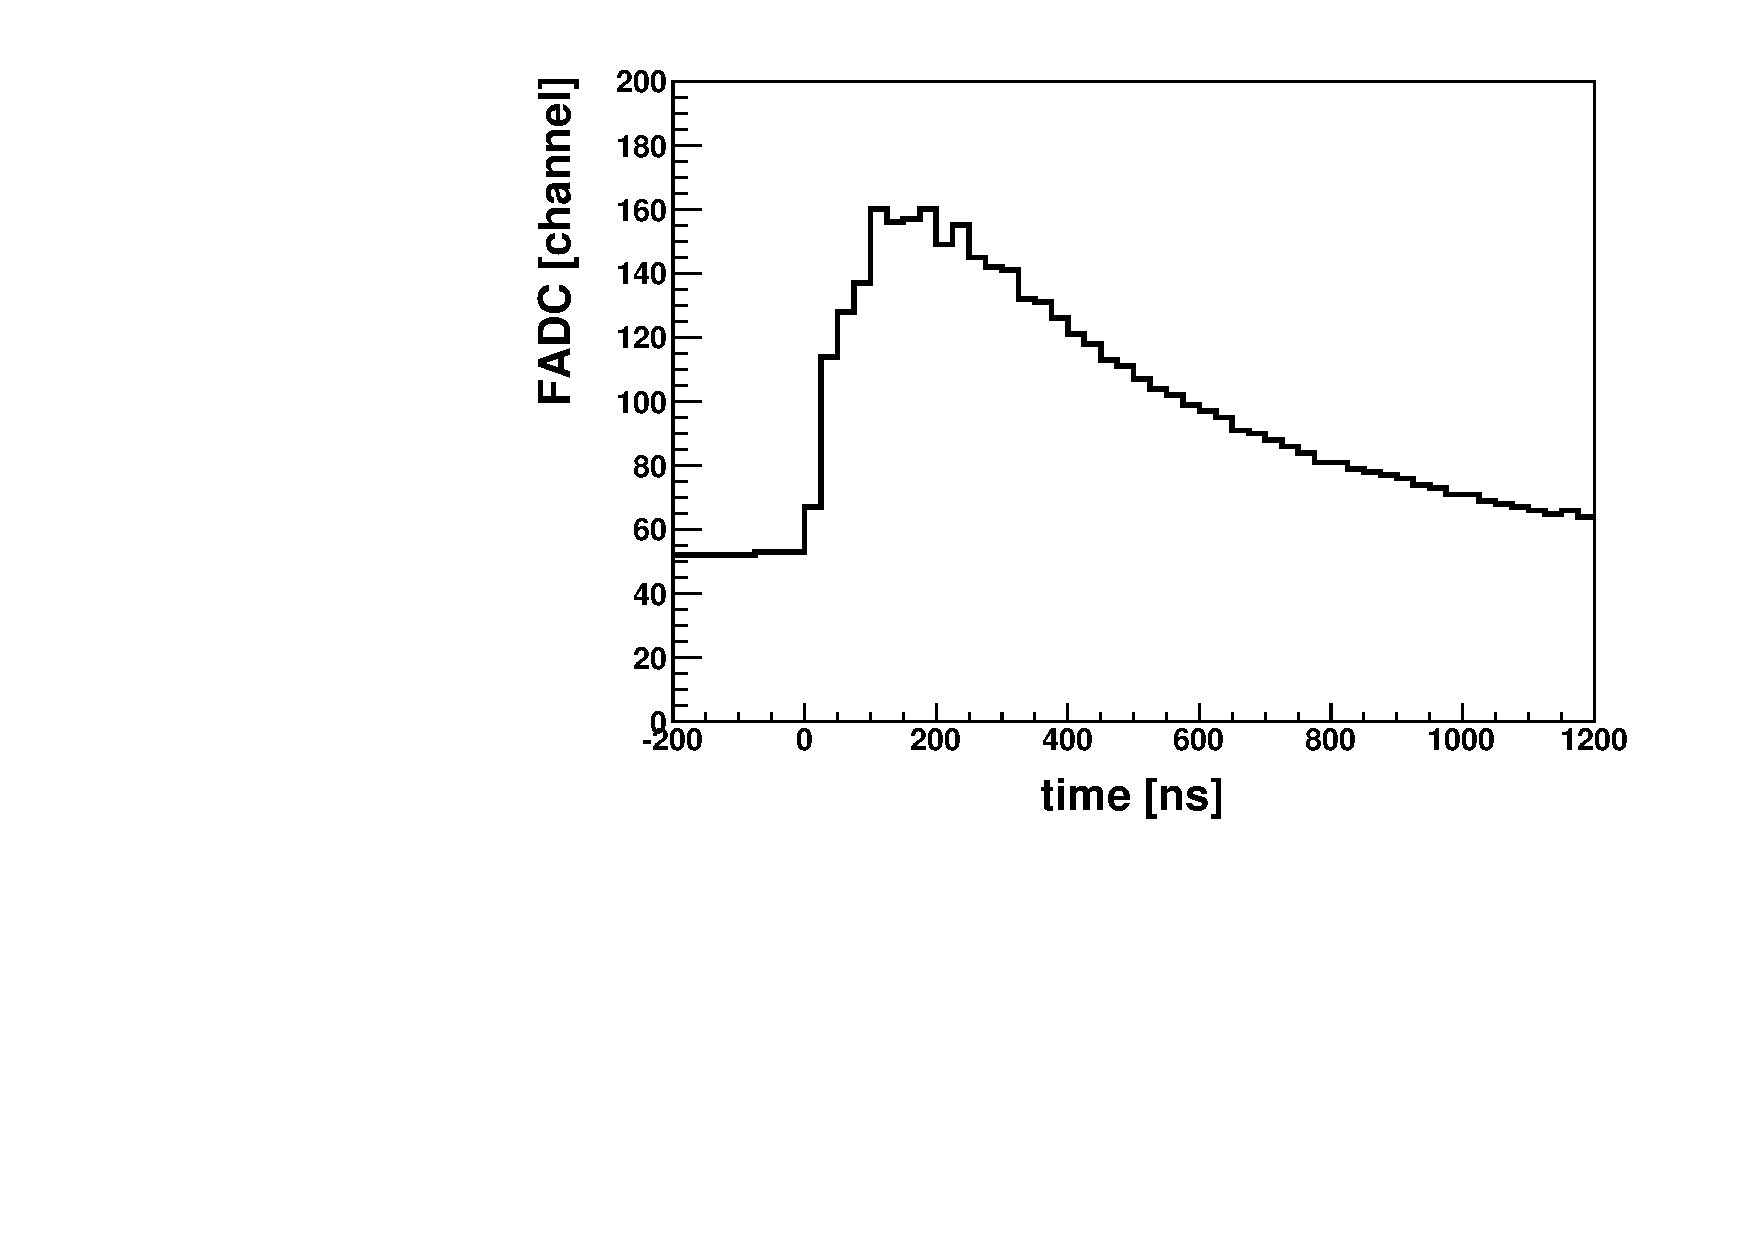
\includegraphics[width=0.47\textwidth]{fig/seleccionAuger/ev1634332_pmt3_dynode.pdf}\\
			\end{array}
			$
			\caption{Ejemplo de un PMT descartado. 
			Estación número 717 (Bobik) en el evento 1634332 detectado el 19 de Septiembre de 2005.
			De arriba hacia abajo PMT's de 1 a 3.
			En la columna izquierda (derecha) se muestra la traza FADC del ánodo (dínodo).
			El PMT's 3 es rechazado por tener una valor de RDA alto.
			}
			\label{fig:event1634332}
			\end{center}
		\end{figure}
		
		
		\subsubsection{Criterios basados en la forma de la señal}
		
		Cuando además de la integral de la señal se presta atención a su salen a la luz otro tipo de patologías que, la mayoría de las veces, dan lugar a un exceso de señal en la traza.
		Para detectar este tipo de PMT's problemáticos se implementa el procedimiento que se detalla a continuación:
		\begin{enumerate}
		 \item Se calculan las integrales de las señales en el dínodo correspondientes a la última mitad de la traza ($\Sigma_i$, con $i$ corriendo sobre los PMT's).
		 \item Se descuenta a cada $\Sigma_i$ el bin de mayor señal y su entorno, para eliminar pulsos generados por muones accidentales.
		 \item Se etiqueta un PMT como dudoso si se cumple:
		 \begin{itemize}
		  \item La estación posee al menos dos PMT's activos\footnote{Las estaciones con 1 solo PMT se analizan m\'as adelante.}.
		  \item El máximo $\Sigma_i$ es mayor a \cant{4}{VEM} y al menos 7 veces mayor que el resto.
		 \end{itemize}
		\end{enumerate}
		
		Si un determinado PMT es etiquetado como dudoso durante un período de tiempo largo se lo considera un indicador de que presenta mal funcionamiento y se lo descarta.
		La figura \ref{fig:event3995196} muestra un ejemplo de este comportamiento. 
		%
		\begin{figure}[h!]
			\begin{center}
			$
			\begin{array}{cc}
			%  \raisebox{0.8\height}{\includegraphics[width=0.4\textwidth]{fig/mapEvent1634332.png}} & 
			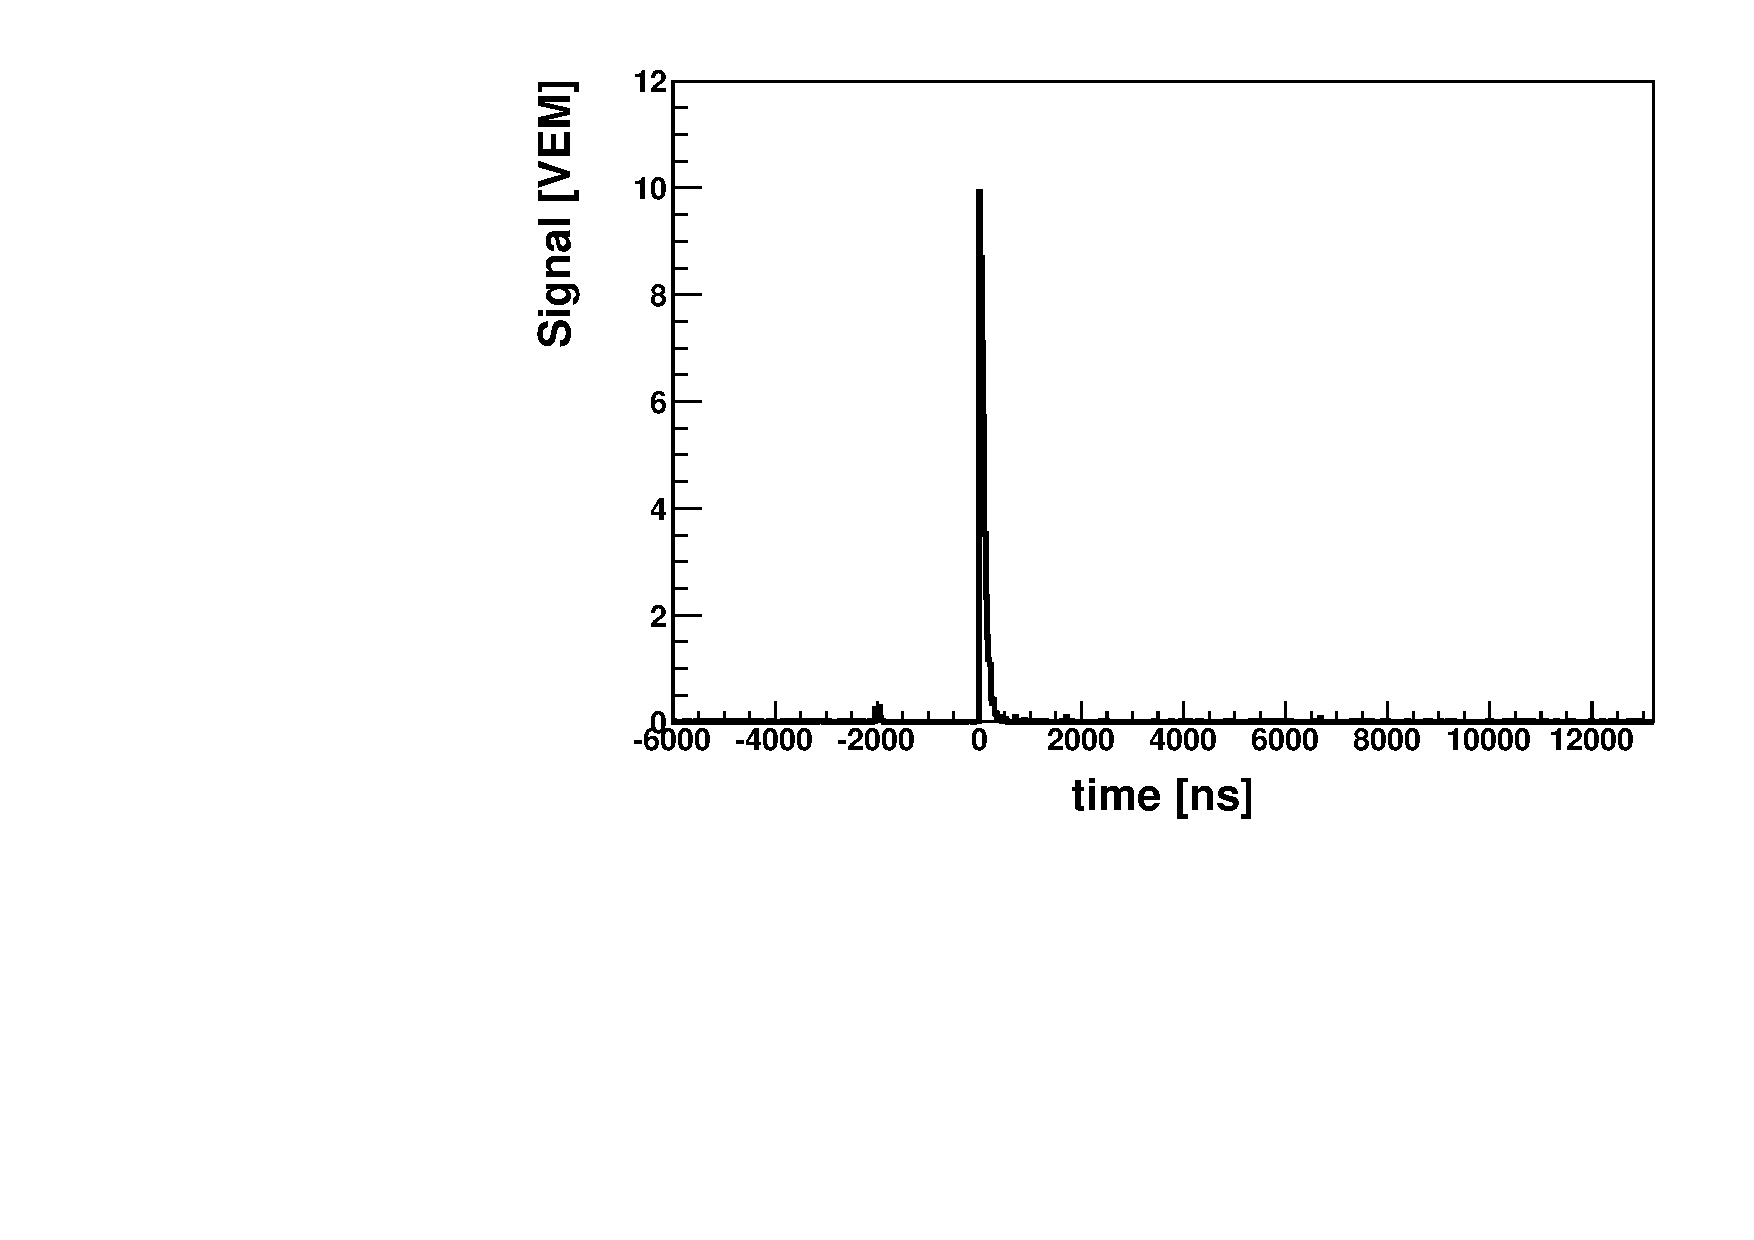
\includegraphics[width=0.6\textwidth]{fig/seleccionAuger/ev3995196_pmt1_anode.pdf}\\
			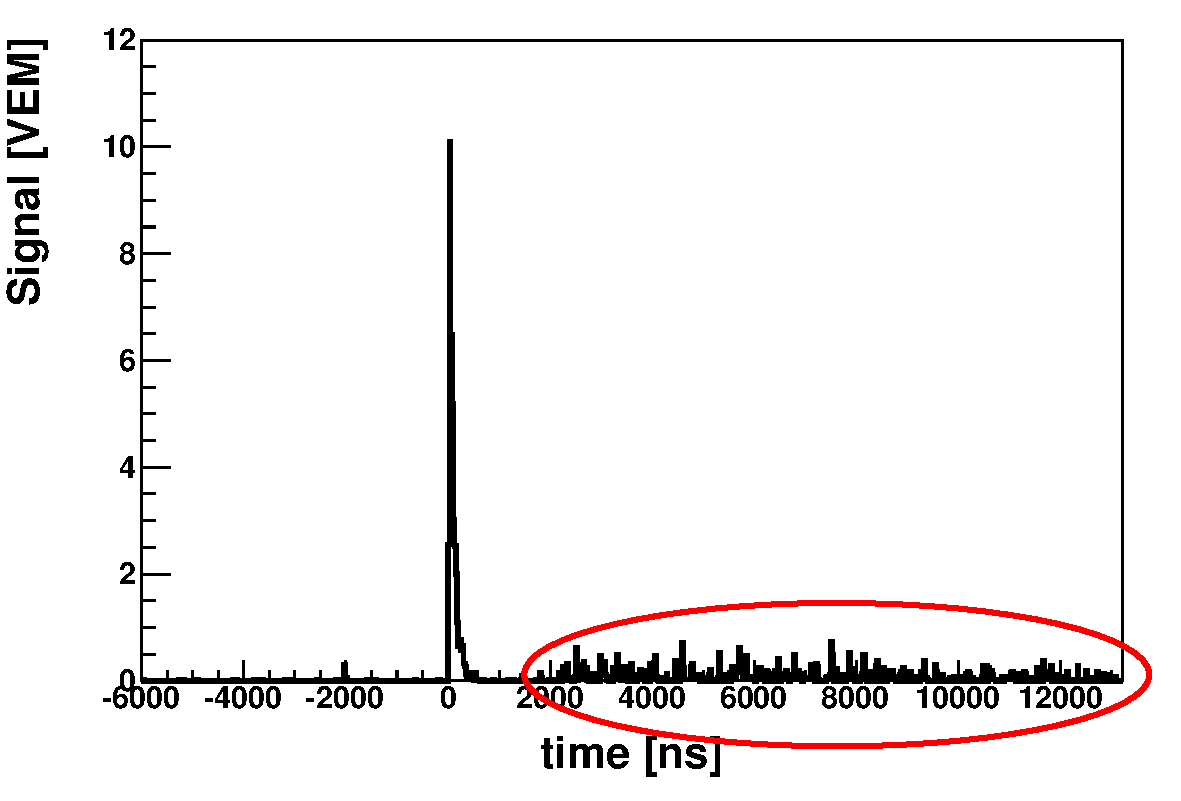
\includegraphics[width=0.6\textwidth]{fig/seleccionAuger/ev3995196_pmt2_anode_withEllipse.pdf}\\
			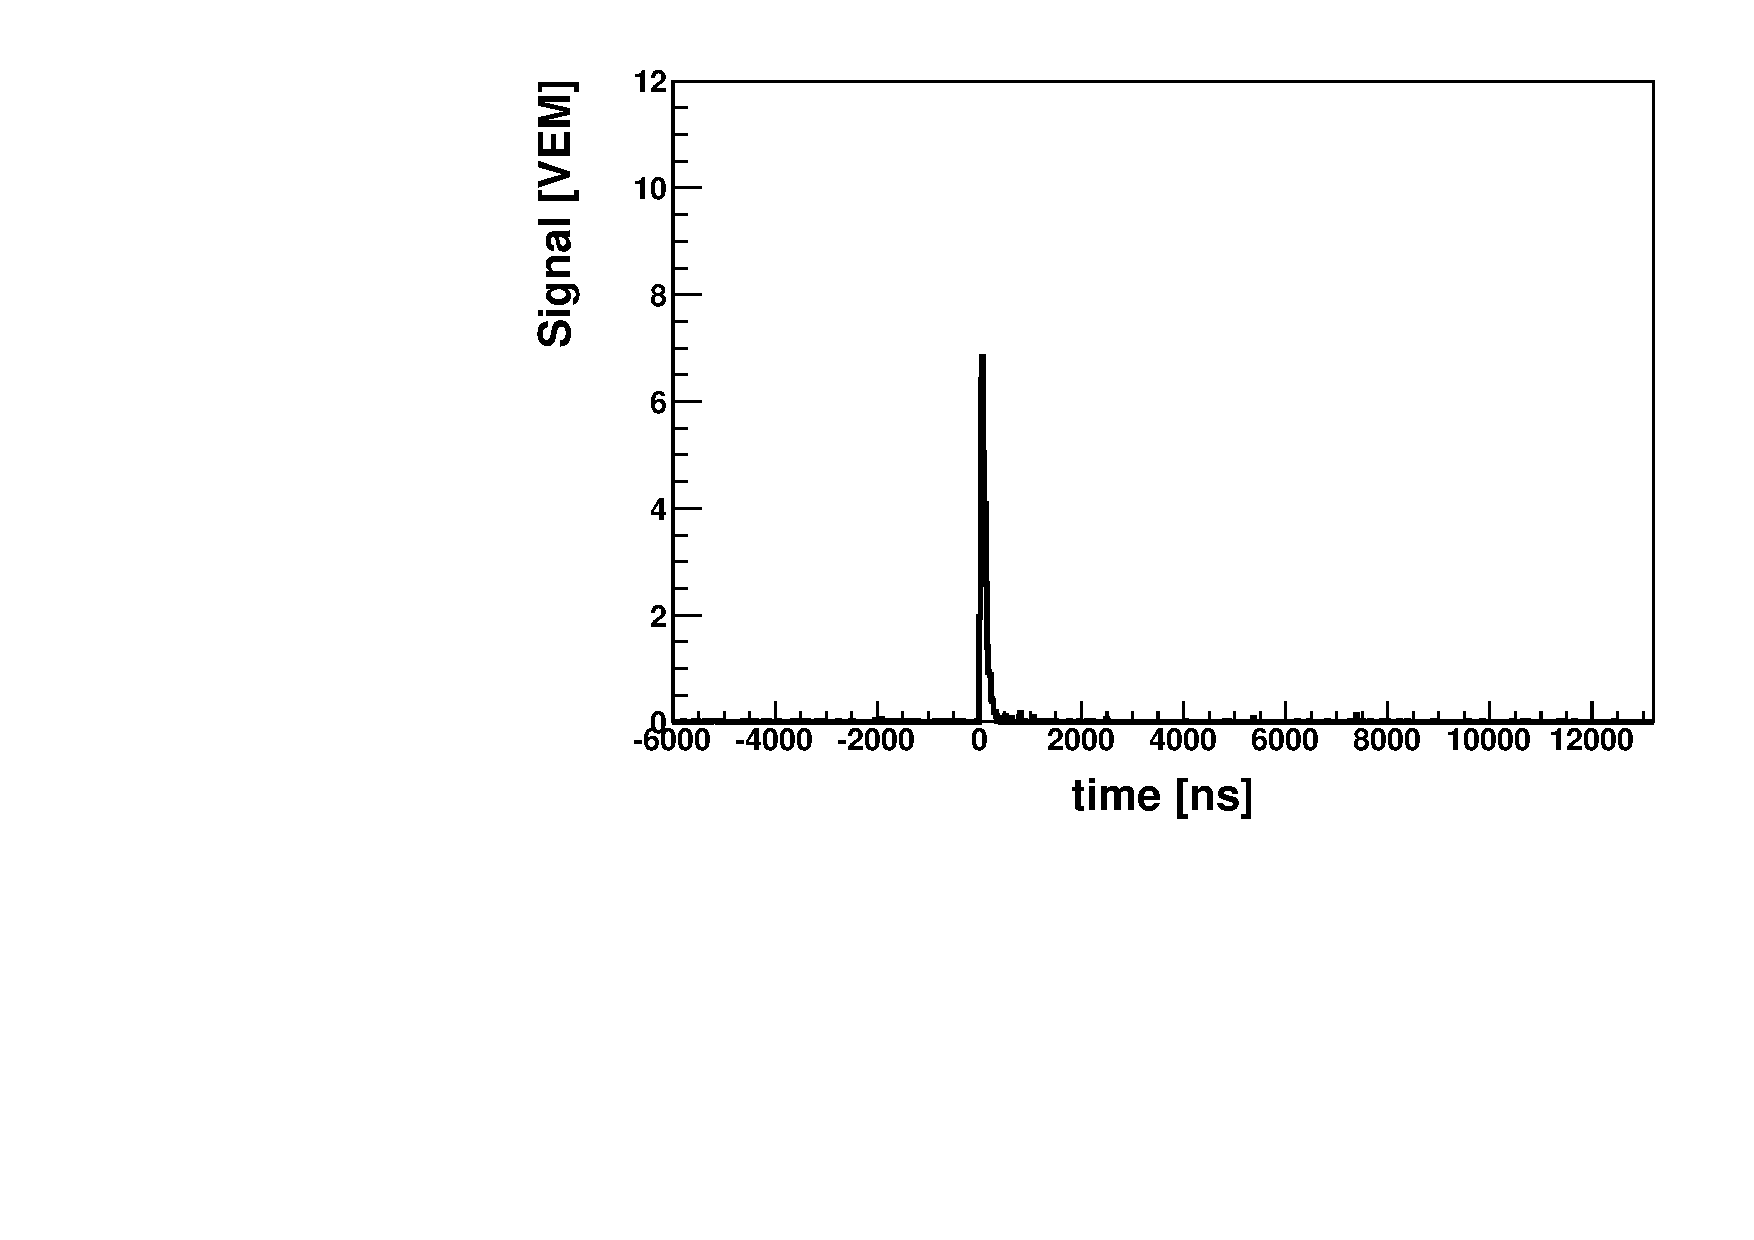
\includegraphics[width=0.6\textwidth]{fig/seleccionAuger/ev3995196_pmt3_anode.pdf}
			\end{array}
			$
			\vspace{-0.5cm}
			\caption{
			Ejemplo de un PMT descartado por permanecer como dudoso por un período largo de tiempo.
			Estación 1440 (Nirvana) para el evento 3995196 con fecha 28 de Septiembre de 2007.
			De arriba a abajo, PMT 1 a 3. El PMT número 2 se etiqueta como dudoso. La etiqueta se debe a la señal espúrea que se señala con una elipse sobre el final de la traza.
			}
			\label{fig:event3995196}
			\end{center}
		\end{figure}

	\subsection{Selección de estaciones}
	
	Hay varias razones para descartar estaciones. Por ejemplo, si algunas de ellas poseen un solo PMT activo durante algún período de tiempo, si cierto evento fue registrado durante una tormenta eléctrica, es posible que la señal de radio emitida por un relámpago haya interferido con la electrónica, o simplemente algún muon accidental disparó la estación que realmente no forma parte del evento.
	A continuación se detallan los procedimientos para detectar este tipo de anomal\'ias.
	
		\subsubsection{Estaciones con un solo PMT activo}
		
		Aunque cada estación cuenta con 3 PMT's algunos pueden tener fallas temporales o permanentes, lo que hace necesario eliminarlos del análisis.
		Dado que la superficie instrumentada es inmensa e incluso a veces de dif\'icil acceso, reemplazar o arreglar un PMT que presenta fallas puede llevar meses.
		Si un candidato a neutrinos apareciera, ser\'ia necesario poder confirmar la señal en la estación por al menos dos PTM's. 
		Si bien no sucede con frecuencia, es posible que suceda que una estación siga funcionando con s\'olo un PMT activo.
		En este caso no sería posible realizar tal confirmación y por ende, debe ser descartada del evento.
		
		\subsubsection{Estación con señales debidas a relámpagos}
		
		Una posible fuente de señales espúreas son los relámpagos.
		Cuando la señal electromagnética que generan alcanza la electrónica de adquisición de las estaciones, se registra una señal oscilante en el orden de los $\rm MHz$, como se observa en la figura \ref{fig:event1186354_st506_pmt3}.
		%
		\begin{figure}[th!]
		\begin{center}
		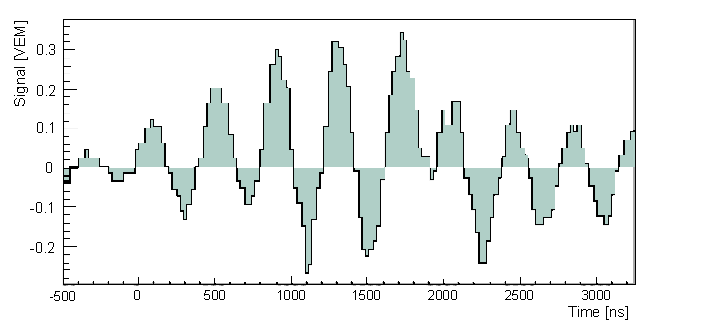
\includegraphics[width=0.7\textwidth]{fig/seleccionAuger/event3995197_station506_pmt3.pdf}
		\caption{Ejemplo de una señal generada por un relámpago.
		La señal corresponde al PMT número 3 del evento 3995197 con fecha 26 de enero de 2005.}
		\label{fig:event1186354_st506_pmt3}
		\end{center}
		\end{figure}
		% 
		La oscilación en la señal se usa para detectar este tipo de sucesos y si un evento contiene una estación de este tipo se lo descarta.
		
		\subsubsection{Estaciones accidentales: efecto de los muones atmosféricos}
		
		El detector se encuentra expuesto a un flujo constante de muones atmosféricos mucho más abundante que el de UHECR\footnote{Estos incluso se utilizan para el calibrado automático de las estaciones.}. 
		Al nivel del detector, \cant{1400}{m} sobre el nivel del mar, éste se compone principalmente de muones en el rango \cant{1-10}{GeV}. 
		Estas partículas, que no forman parte de los eventos que nos interesan, pueden afectar la reconstrucción de dos maneras:
		%
		\begin{enumerate}
		\item \textbf{Producir un trigger T2 en una estación de superficie que no pertenece al evento:} como las partículas que disparan la estación no pertenecen a la lluvia, el tiempo del T2 adicional tendrá una distribución uniforme en la ventana de 60~$\mu$seg del T3. Como la selección de lluvias inclinadas depende fuertemente de las posiciones y tiempos de disparo de las estaciones, una estación extra puede dar como resultado una incorrecta estimación de la geometría de la lluvia, especialmente en los eventos más pequeños.

		\item \textbf{Agregar señal espurea en alguna de las estaciones que sí pertenecen al evento:} si la señal accidental ocurre algunos $\rm\mu$seg antes o despues de que las partículas de la cascada atmosférica alcancen la estación el resultado es que ambas señales se fusionan en una misma traza, modificando sus observables.
		Como se discutirá más adelante en este capítulo, este fen\'omeno puede ser importante y será tenido en cuenta en la elaboración del criterio de identificación de neutrinos. 
		Por otro lado, si la señal espurea es la que fija el tiempo de disparo del T2 (ver figura \ref{fig:trazaMalTiempo}), la reconstrucción geométrica del evento también se verá afectada.
		\end{enumerate}
		%
		\begin{figure}[ht]
		\begin{center}
		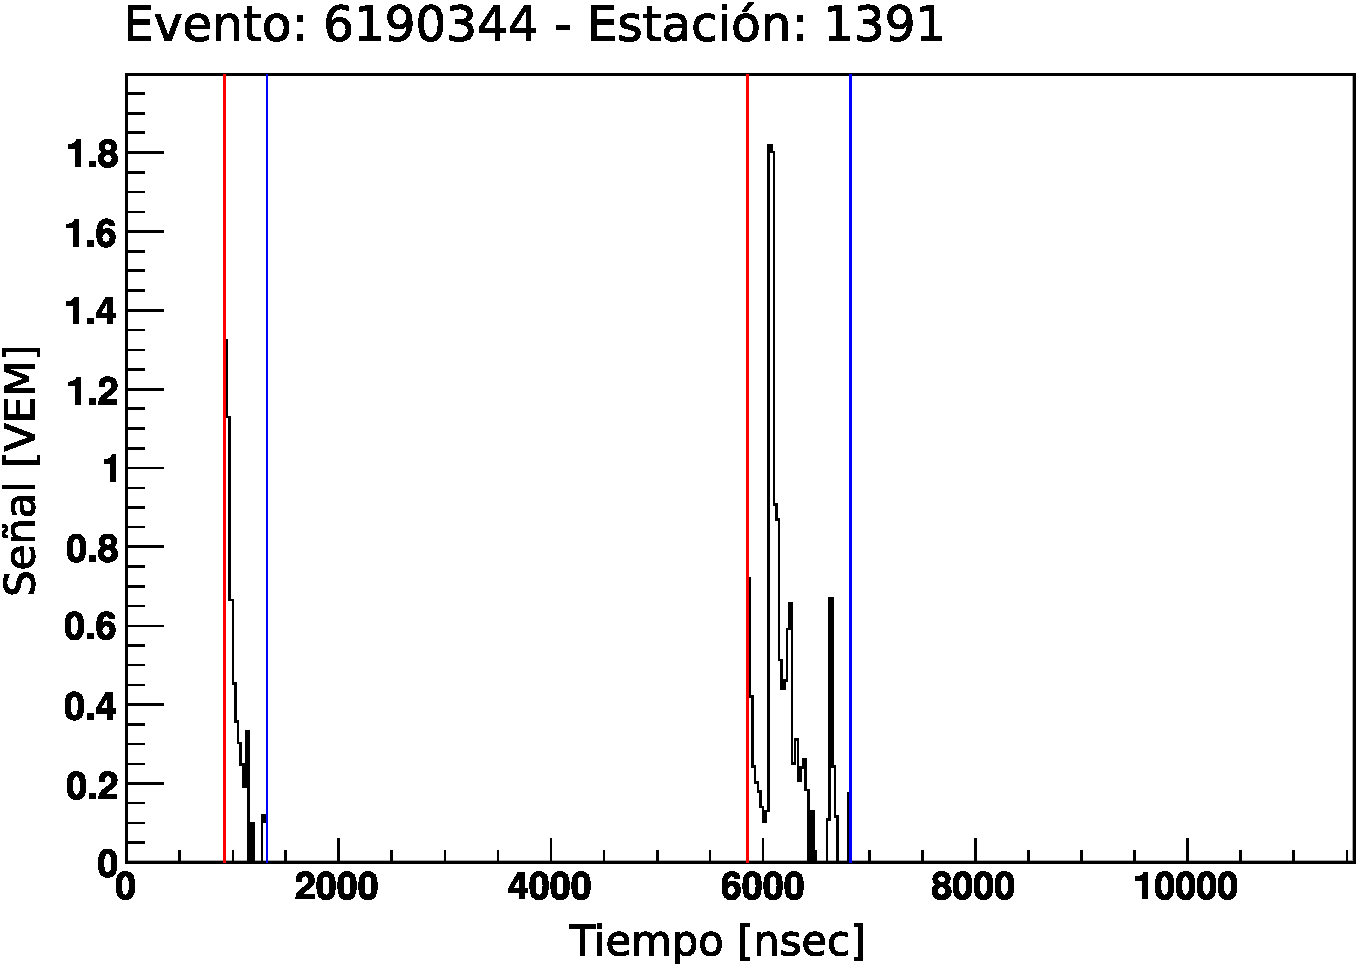
\includegraphics[width=0.75\textwidth]{fig/seleccionAuger/badStartTime.pdf}
		\caption{Efecto de un muón accidental en la determinación errónea del tiempo de disparo. El etiquetado se realizó mediante el algoritmo de limpieza de traza (ver texto).}
		\label{fig:trazaMalTiempo}
		\end{center}
		\end{figure}
		%
		Entonces, con el fin de minimizar el impacto de estas señales espureas se aplica el procedimiento que se describe a continuaci\'on.
		
		\titulo{Algoritmo de limpieza de traza} la cantidad de energía que los muones depositan en el tanque es, a primer orden, proporcional a la longitud del camino que recorren dentro del mismo.
		Dado que las estaciones son bastante más anchas que altas (\cant{1.2}{m} de alto por \cant{3.6}{m} de diámetro), los muones inclinados producir\'an entonces una señal, en promedio, mayor que los verticales.
		Si adem\'as se tiene en cuenta que los muones accidentales son mayormente verticales (como se puede ver figura \ref{fig:atmo_mu_flux}) y ocurren aleatoriamente, es posible definir un procedimiento que identifique qué fracción de la traza debe ser eliminada.
		%
		\begin{figure}[ht]
		\begin{center}
		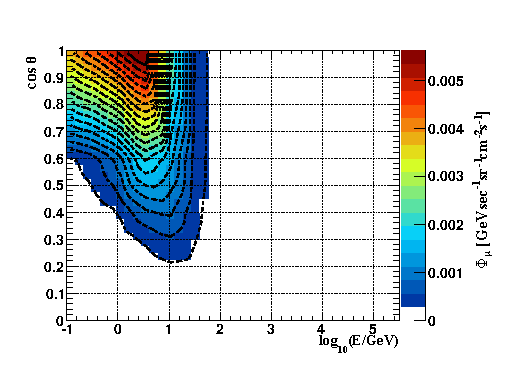
\includegraphics[width=0.85\textwidth]{fig/seleccionAuger/atmo_mu_flux.pdf}
		\caption{Flujo de muones atmosféricos de acuerdo con la parametrización dada en~\cite{cite:atmo_mu}. Puede observarse que la mayoría presenta un ángulo cenital inferior a 50$^{\circ}$ ($\cos\theta \geqslant 0.6$)}.
		\label{fig:atmo_mu_flux}
		\end{center}
		\end{figure}
		
		El algoritmo de limpieza utilizado fue desarrollado por el grupo de la UBA en el marco del an\'alisis de DGH y tomado por el de ES~\cite{trace_cleaning,cite:tesisJavier,cite:tesisYann}.
		Este comienza al nivel de cada PMT dentro del tanque y se procede como se describe a continuaci\'on:
		%
		\begin{enumerate}
		 \item Se extraen los segmentos de señal de cada PMT, definidos por al menos 2 bines consecutivos que presenten al menos 3 unidades de FADC sobre la linea de base.
		 Se guardan los índices de inicio y fin, y se calcula su carga $Q$ y su pico $P$.
		 \item Se unen segmentos contiguos si el gap entre ellos es de menos de 20 bines más la longitud del primero, y si al menos una de las siguientes condiciones se cumple:
		 \begin{enumerate}
		  \item El primer segmento posee una señal $Q_n>0.3Q_{n+1}$
		  \item El segundo segmento posee menos de 5 unidades FADC sobre la línea de base
		 \end{enumerate}
		El objetivo de estas condiciones es unir los que hayan sido provocados por partículas de la lluvia.
		\item Se promedian las señales de los diferentes PMT's.
		\item El start time de los segmentos combinandos se toma de la contribución que posea la mayor señal.
		\end{enumerate}
		
		Como ejemplo, en la figure \ref{fig:trazaMalTiempo}, el algoritmo encuentra dos segmentos.
		En principio, el segmento con la señal integrada más grande se conserva y el resto se descarta.
		Sin embargo, tambien podría ocurrir que uno o más segmentos posean una señal similar, por lo que no sería claro cuál es el segmento que realmente interesa.
		Para salvar estas situaciones, se aplica un algoritmo especial, que comienza segmentando la señal promedio deos PMT\'s con un criterio similar al que se aplica para segmentar la de los individuales:
		%
		\begin{enumerate}
		 \item El segmento comienza con el primer bin que presente una señal por encima de los \cant{0.2}{VEM}.
		 \item En los siguientes 10 bines (\cant{250}{ns}) la carga integrada $Q$ debe superar los \cant{3}{VEM}. Si no, el inicio de la traza se mueve un bin hacia adelante hasta que las ambas condiciones se cumplan.
		 \item El final de la señal se define cuando a partir de él se encuentren 15 bines consecutivos por debajo de \cant{0.2}{VEM}.
		 \item Se calculan dos cantidades:
		 \begin{enumerate}
		  \item $nBoT$: el número de bines por encima de \cant{0.2}{VEM}.
		  \item $Q_T$: la suma de la señal en los bines sobre \cant{0.2}{VEM}.
		 \end{enumerate}
		\end{enumerate}
		%
		A cada segmento se le asigna una puntuación $s=nBoT\times Q_T$. 
		Las trazas inducidas por muones atmosféricos tienden a tener valores de $s$ pequeños cuando se los compara con las inducidas por lluvias inclinadas.
		Si hubiera más de un segmento que cumpla $s>0.5s_{max}$, con $s_{max}$ la máxima puntuación, la estación es rechazada debido a que el tiempo de inicio de la señal es ambiguo.
		En caso contrario, el segmento con mayor puntuación se conserva y el resto se rechaza.
		La figura \ref{fig:multipicos} muestra un ejemplo de una estación que presenta tres segmentos similares. Esta estación es removida del evento antes de aplicarle la reconstrucción.
		%
		\begin{figure}[ht]
			\begin{center}
			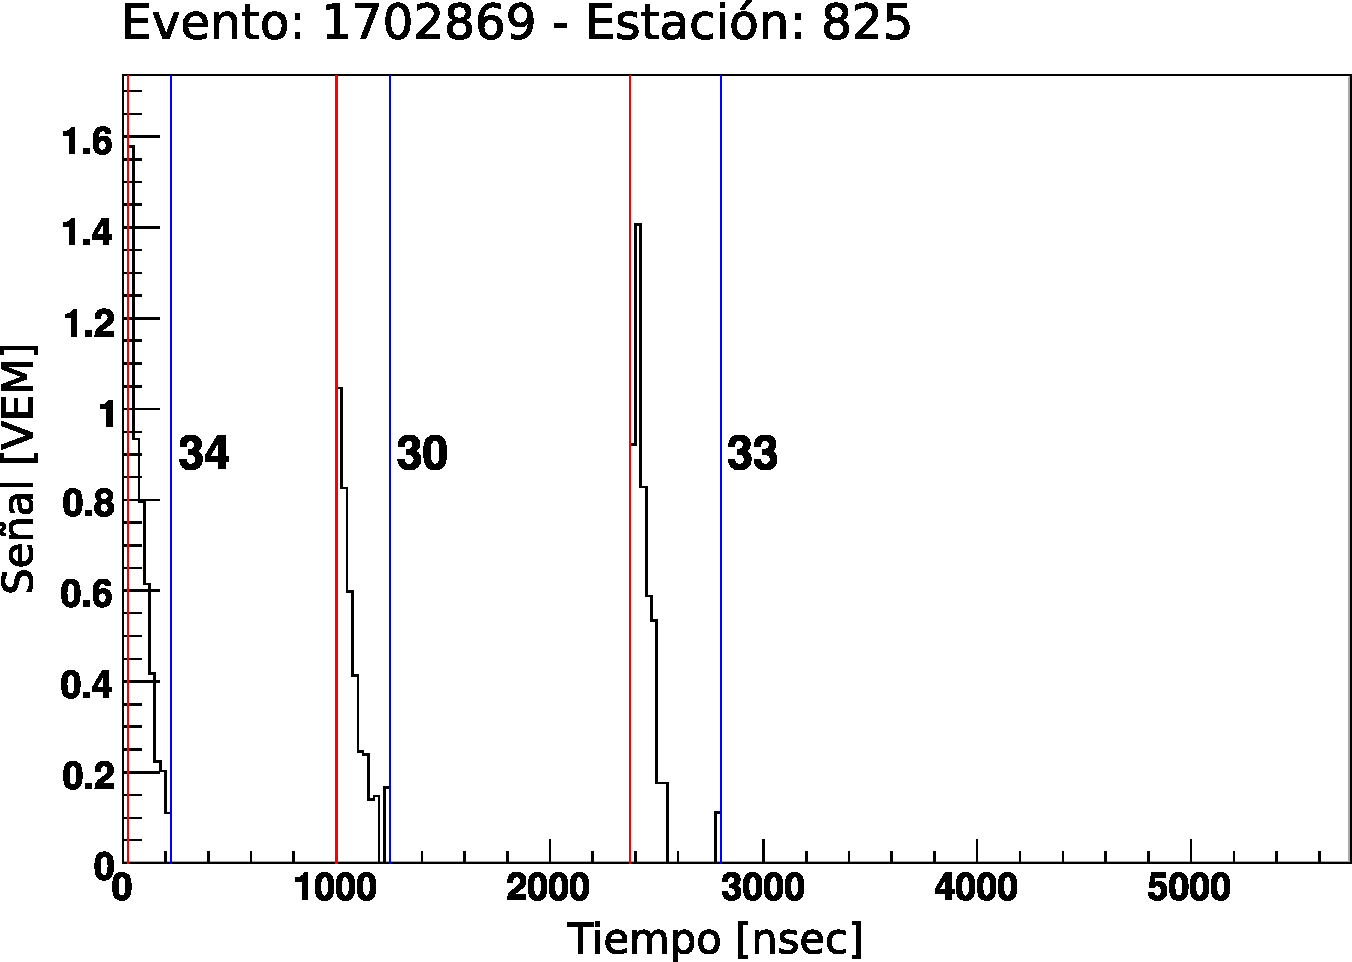
\includegraphics[width=0.75\textwidth]{fig/seleccionAuger/multipicos.pdf}
			\caption{Traza que presenta múltiples segmentos de señal con características similares en la que no es posible determinar el tiempo de disparo T2. Los valores resaltados indican el puntaje asignado a cada segmento.}
			\label{fig:multipicos}
			\end{center}
		\end{figure}
		%
		
		
	\subsection{Reconstrucción preeliminar}
	
	Una vez aplicados los procedimientos hasta aquí descriptos, los eventos consisten en una lista de estaciones cuyos tiempos de disparo T2 se encuentran bien definidos.
	Sin embargo, todav\'ia puede existir entre ellas algunas disparadas por muones atmosféricos o incluso por una lluvias de baja energía.
	Con el fin de descartar estas estaciones espureas se impone una serie de requisitos de compacticidad espacial y temporal sobre los tiempos de disparo del evento.
	
	\subsubsection{Eliminación de estaciones aisladas} 
	
	El primer paso es remover las estaciones aisladas pidiendo las siguientes dos condiciones:
	\begin{enumerate}
	 \item Criterio estandar: Se elimina una estación como aislada si no cumple que:
	 \begin{enumerate}
	  \item Existe una estación con T2 a menos de tres coronas, \cant{d_1\leq4700}{m}, y dentro de un rango temporal de compatible con un frente que se desplaza a la velocidad de la luz, $t_1=\frac{d_1}{c}$ (\cant{\sim15700}{ns} para el caso de 3 coronas).
	  \item Existe adem\'as una segunda estación con T2 dentro de la cuarta corona, \cant{d_2\leq6200}{m}, y con el mismo criterio temporal, \cant{t_2=\frac{d_2}{c}\sim20700}{ns} cuando la separacion sea de 4 coronas.
	 \end{enumerate}
% 	 \item Eliminación de señales muónicas: Si la magnitud de la traza es compatible con la señal de un mu\'on vertical, ${\rm AoP} \equiv \frac{S}{S_{peak}}<1.4$, el criterio es m\'as estricto, pidiendo al menos una señal con T2 en la primer corona o en las estaciones cercanas de la segunda, \cant{d\leq2700}{m}.
	\end{enumerate}
	
	\subsubsection{Selección Top-Down} 
	
	El segundo paso consiste en seleccionar las estaciones cuyos tiempos de disparo son compatibles con el pasaje del frente de part\'iculas de una EAS.
	El algoritmo utilizado para este propósito se conoce como \emph{selección Top-Down} \cite{topDownSel}.
	La idea general del método se basa en ir descartando las estacionesmenos veros\'imiles hasta encontrar una configuración satisfactoria.
	A continuación se expone paso a paso del algorítmo:
	%
	\begin{enumerate}
	 \item Se realiza una reconstrucción del ángulo cenital del evento, $\theta_{rec}$, asumiendo un frente plano y un tiempo de arribo $t_0$, definido como el tiempo promedio de inicio de señales pesado por las mismas. Este procedimiento se realiza anal\'iticamente como se detalla en el apéndice \ref{ap:topDown}
	 \item Se determina la compatibilidad temporal de cada estación del evento requiriendo:
	 \begin{itemize}
	  \item $\Delta t_i < (N-2)\cdot 250{\rm ns} \cdot {\rm max}(\cos\theta_{rec},0.2)$
	  \item $\sum_i\Delta t_i^2 < \left[(N-2)\cdot 200{\rm ns} \cdot {\rm max}(\cos\theta_{rec},0.2)\right]^2$
	 \end{itemize}
	 donde $\Delta t_i$ es la diferencia entre el tiempo de T2 de la estaci\'on $i$ y el obtenido mediante el ajuste del frente plano.
	 
	 Estos cortes dependen de la multiplicidad del evento $N$ y del ángulo reconstruido $\theta_{rec}$.
	 La dependencia en $N$ aparece debido a la curvatura del frente de la lluvia, las estaciones perisfericas suelen presentar una mayor diferencia temporal respecto del frente plano que las centrales (ver figura \ref{fig:planeFrontAprox}).
	 Este efecto se vuelve m\'as notorio a medida que aumenta $N$.
	 Por otra parte, la dependencia del radio de curvatura $R$ con el ángulo cenital aparece por una razón similar: las lluvias inclinadas llegan al detector tras atravesar mayor cantidad de materia que las verticales. Por este motivo, la dependencia del radio del frente de la lluvia se considera típicamente $R\propto\sec\theta$ \cite{cite:ShowerFront}.
	 Consecuentemente, para ángulos cenitales grandes el frente de la lluvia presentar\'a una curvatura pequeña ($R$ grande).
	 Adem\'as, para $\cos\theta < 0.2$, lo que corresponde a $\theta>80^\circ$, se asume que el mismo ha alcanzado su curvatura mínima.
	 Por esta raz\'on, el mínimo tiempo de tolerancia utilizado para las estaciones respecto del frente plano será \cant{(N-2)50}{ns}.
	 \item Tambien se pide compacticidad espacial.
	 Todas las estaciones, proyectadas sobre el plano del frente de la lluvia, deben estar contenidas dentro de un círculo de radio $r_{max}$, con:
	 \begin{equation}
	  r_{max} = \sqrt{1300^2(N-2)}{\rm m}
	 \end{equation}
	 \item Se eval\'ua la condición de T3.
	\end{enumerate}
	%
	\begin{figure}[ht]
	\begin{center}
	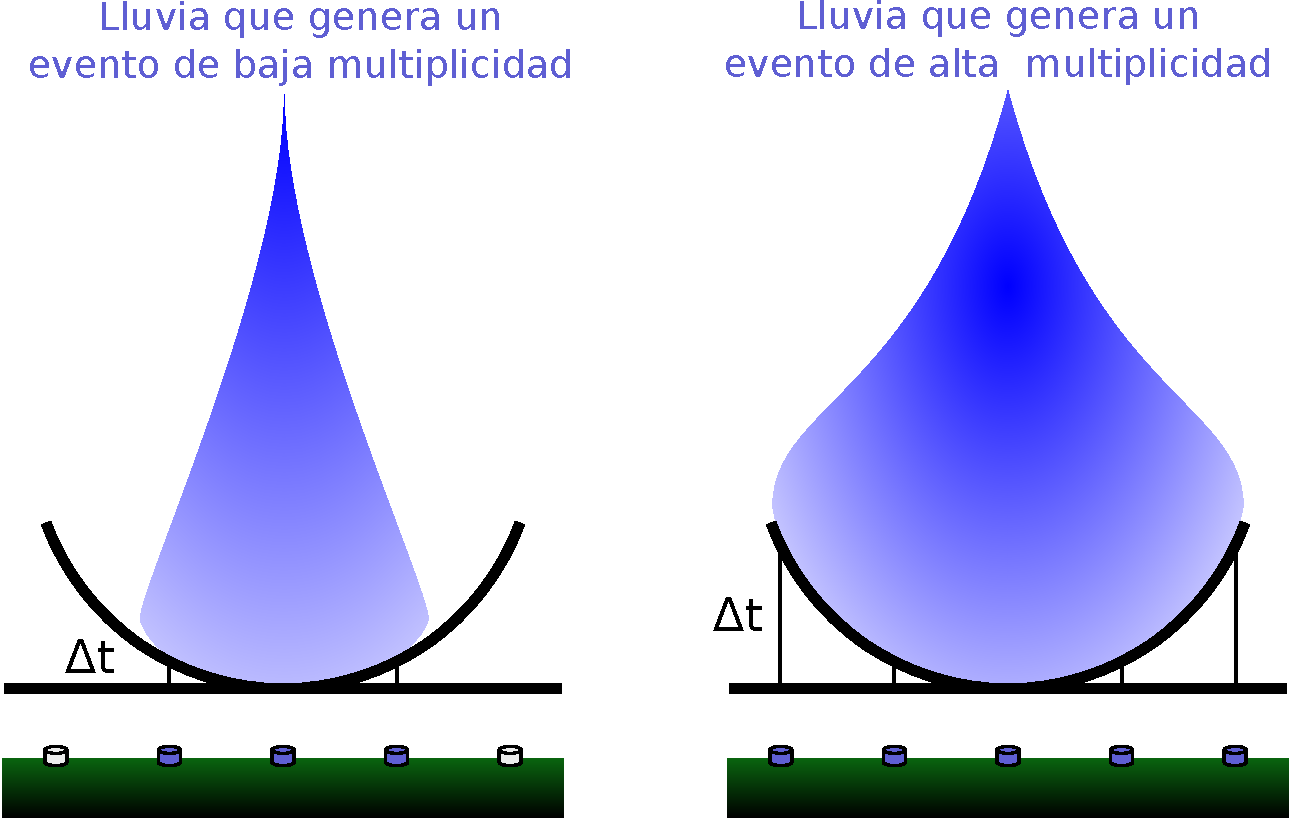
\includegraphics[width=0.85\textwidth]{fig/seleccionAuger/plano_vs_curvo.pdf}
	\caption{Esquema de la diferencia de tiempo entre un frente de lluvia curvo y su aproximación plana. 
	Las lluvias que generan alta multiplicidad de estaciones tienden a presentar diferencias de tiempo mayores al compararlas con la aproximación de frente plano.}
	\label{fig:planeFrontAprox}
	\end{center}
	\end{figure}
	%
	Si alguna de las condiciones no se satisface se intenta con las configuraciones de $N-1$ estaciones, quitando primero las de menor señal. 
	En cuanto todos los criterios se satisfacen, se acepta la configuración. Si esto no sucede, se quitan 2, 3 o hasta 4 estaciones.
	Si luego de probar todas estas configuraciones, quitando hasta 4 estaciones, ninguna cumpli\'o los criterios, el evento se descarta debido a la alta probabilidad de tener una mala reconstrucción.
	
	En caso de que todos los tanques se encuentren alineadas, no es posible realizar la reconstrucción antes mencionada.
	En su lugar, se calcula la velocidad aparente de la señal $v_{ij}$ para cada par de estaciones $(i,j)$ con trigger T2:
	%
	\begin{equation}
	 V_{ij}=\frac{d_{ij}}{\Delta t_{ij}}
	\end{equation}
	%
	donde $d_{ij}$ es la distancia entre estaciones y $\Delta t_{ij}$ es la diferencia entre los tiempos de disparo.
	Luego, a partir de los valores de $V_{ij}$ se calcula la velocidad promedio $\langle V\rangle$ y la compatibilidad temporal se eval\'ua para cada estación con la siguiente condición:
	%
	\begin{equation}
	 \frac{V_{ij}-\langle V\rangle}{\langle V\rangle}\leq0.1
	\end{equation}
	
	
	\subsection{Criterios adicionales}
	
	Una vez que las estaciones con señales espureas han sido descartadas, se eval\'uan algunos criterios de compacticidad adicionales que aseguran una mejor reconstrucción de la lluvia.
	
	\begin{enumerate}
	 \item \texttt{6T5}: es el criterio estandar del observatorio, que pide que la estación con mayor señal se encuentre rodeada por 6 estaciones activas. Sólo se aplica en la búsqueda de DGL.
	 \item \texttt{isContained}: una vez reconstruido el baricentro de la lluvia se selecciona la estación m\'as cercana y se requiere que se encuentre rodeada por 5 estaciones activas. Esta condici\'on es requisito en las búsquedas de DGH y ES, y es algo más laxa que el \texttt{6T5}\footnote{Esta permite que el baricentro de la lluvia caiga algo más afuera de los bordes del detector.}. 
	 Dado que en estas búsquedas la contaminación debido al fondo es menos frecuente que para el rango angular que observa DGL, resulta posible relajar levemente el \texttt{6T5}.
	 \item \texttt{6T5 posterior}: igual que \texttt{isConteined} pero pidiendo que la estación seleccionada se encuentre rodeada por 6 estaciones activas. Solo se aplica a DGL.
	 \item \texttt{hottestHasNeighbour}: se pide que la estación de mayor señal tenga en su primer corona otra estación con T2. El objetivo de este corte es evitar eventos de baja multiplicidad con ``agujeros''. Esta condición s\'olo se eval\'ua en el análisis de ES.
	\end{enumerate}
	
\section{Selecci\'on de lluvias inclinadas}

Una vez obtenida la muestra de eventos de calidad, se encuentran dadas las condiciones para aplicar la selección de eventos inclinados.
Para ello se consideraron variables de tipo directas e indirectas, a saber:
\begin{enumerate}
 \item Directas: consisten en los distintos valores del parámetro $\theta$ obtenidos a partir de ajustar los tiempos de disparo de las estaciones con diferentes modelos de frente de onda (plano, cónico, esférico, parabólico, etc.)
 \item Indirectas: se refieren a otras variables sensibles a la inclinación, como por ejemplo la velocidad aparente de la señal o la elongación de la ``huella'' dejada por la lluvia sobre el detector.
\end{enumerate}
	
	\subsection{Reconstrucción angular}
	\label{sbsc:thetaRec}
	
	Para obtener un estimador del ángulo cenital se aplica un procedimiento iterativo.
	Como primer paso, sobre el conjunto de estaciones seleccionadas se realiza un ajuste asumiendo un frente plano.
	Este ajuste, más sofisticado que el que se realiza en la selección de estaciones, utiliza un modelo para la incerteza en el tiempo de disparo \cite{cite:ines} optimizado para lluvias inclinadas:
% 	Este modelo fue optimizado para describir lluvias horizontales hadrónicas iniciadas alto en la atmósfera en las que, por lo tanto, domina la componente muónica al nivel del detector (eventos inclinados típicos):
	%
	\begin{equation}
	\sigma_t = 20 \left[ 1 + \left( \frac{15}{S} \right)^{2/4.5} \right]
	\label{ec:varT} 
	\end{equation}
	%

% 	Es importante resaltar que, al utilizar este modelo, se elige priorizar la correcta reconstrucción de las lluvia hadrónicas (inmensa mayoría, si no la totalidad, de los datos) por sobre las posibles lluvias profundas iniciadas por neutrinos
% 	\footnote{Las lluvias profundas cuentan con una componente EM apreciable al alcanzar la tierra, lo que produce que la incerteza en su tiempo de disparo no sea correctamente descripta por el modelo anterior que asume que la cantidad de electrones y fotones es despreciable.}. 
	
% 	\textbf{CHARLAR SOBRE ESTO}
% 	Como se discutirá más adelante en la Sec.~\ref{sub:thetaRec}, esta elección produce una disminución en la eficiencia de detección de neutrinos pero se ve justificada ya que implica una disminución del fondo hadrónico debido a lluvias ``verticales'' ($\theta<75^\circ$) incorrectamente reconstruidas como ``horizontales'' ($\theta>75^\circ$).

	Una vez realizada la reconstrucción se evalúan las diferencias de tiempo $\Delta t_i$ entre las estaciones y el frente plano obtenido.
	Si alguno de los $\Delta t_i$ no está contenido en el intervalo [-300,700]~$\mbox{ns}$~\footnote{
	Una vez producidos, los muones viajan sin desviarse y, en general, alcanzan la tierra antes que la componente EM. 
	Las fluctuaciones en su tiempo de arribo son entonces menores a las esperadas para electrones y fotones que sufren multiples disperciones en su camino.
	Esta es la razón de que se tome un intervalo asimétrico.
	},
	la estación con mayor $\Delta t_i$ es removida y se repite la reconstrucción.
	Este procedimiento continua hasta que se encuentra una configuración aceptable o, si tras alguna de las iteraciones quedasen menos de 4 estaciones, se lo rechaza.
	
	Si el evento está constituido por estaciones alineadas, el ángulo azimutal es fijado en la dirección de avance de la señal y se aplica el mismo procedimiento de reconstrucción ya descripto.
	En el caso de eventos en linea el ángulo cenital obtenido es, en realidad, una cota mínima (ver figura~\ref{fig:conoLineEvent}).
	%
	\begin{figure}[ht]
	\begin{center}
	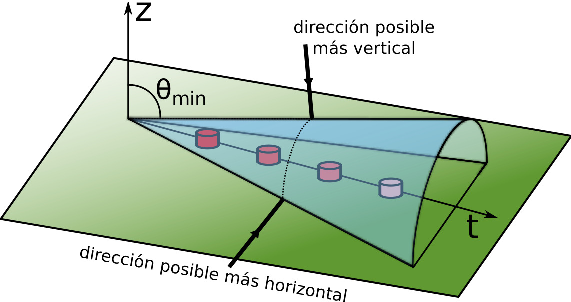
\includegraphics[width=0.75\textwidth]{fig/seleccionAuger/conoLineEvent.pdf}
	\caption{Esquema de reconstrucción geométrica de un evento en l\'inea. Una cota mínima para el ángulo cenital se obtiene al considerar que el ángulo azimutal de la lluvia coincide con la l\'inea que une las estaciones.}
	\label{fig:conoLineEvent}
	\end{center}
	\end{figure} 
	
	En la figura \ref{fig:resDGL} se muestra la resolución angular obtenida para lluvias DGL iniciadas por $\nu_e$ via CC, que se define como la desviación estandar de la diferencia entre el ángulo reconstruido y el simulado, $(\theta_{Rec}-\theta_{MC})$.
	%
	\begin{figure}[ht]
	\begin{center}
	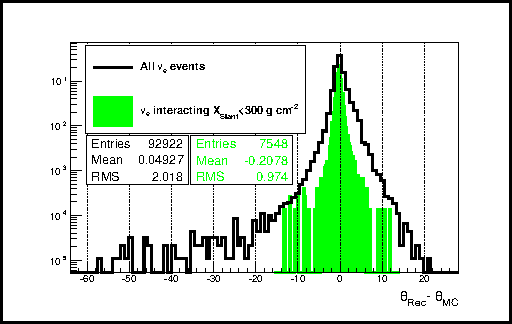
\includegraphics[width=0.75\textwidth]{fig/seleccionAuger/resDGL.pdf}
	\caption{Resolución angular para lluvias DGL. En verde se resaltan los eventos iniciados alto en la atmósfera. Estos presentan una resolución debido a que el método de ajuste se encuentra optimizado para eventos hadrónicos.}
	\label{fig:resDGL}
	\end{center}
	\end{figure}
	%
	En verde se resaltan los eventos iniciados alto en la atmósfera (\cant{D<300}{g cm^{-2}}), que presentan mayor resolución. 
	Esto se debe a que el método utilizado se encuentra optimizado para eventos hadrónicos, que se inician a una profundidad media de \cant{\sim100}{g cm^{-2}}.
	
	Dado que el problema esta mal condicionado para lluvias muy horizontales ($\sim90\deg$), no es posible utilizar esta clase de variables en la búsqueda de neutrinos ES.
	Para salvar este problema es necesario utilizar variables que no dependan de este tipo de ajuste, lo que se desarrolla en la sección \ref{sc:otrasVarIncl}.
	Por otra parte, existe adem\'as cierto tipo de configuraci\'on espacial de los tanques particularmente propensa a producir una reconstrucci\'on angular erronea.
	
	\subsubsection{Eventos espacialmente mal condicionados}
	\label{sub:illEvents}
	Definimos a un evento como ``espacialmente mal condicionado'' cuando está formado por un evento en linea más una estación no alineada. En otras palabras, es un evento no alineado que se vuelve en linea al remover una sola estación.
	Este configuración espacial es particularmente susceptible a producir una mala reconstrucción espacial. Para entender porqué, es útil considerar un caso límite: un evento totalmente vertical que dispara tres estaciones alineadas. En este caso, las tres estaciones tienen el mismo tiempo de T2 por lo que si se lo reconstruye como evento en linea se obtendría un ángulo cenital consistente con un evento vertical. Sin embargo, en el caso de que junto con el evento ocurriera el disparo de una estación accidental no alineada, el evento se reconstruiría como no alineado y el ángulo cenital sería determinado sólo por el tiempo de la estación extra. En resumen, una sola estación sería la que determinaría la geometría reconstruida del evento.

	Para evitar este problema, los eventos que presentan una configuración espacial mal condicionada se someten a una selección adicional. 
	Se ignora la estación no alineada, se reconstruye el evento en línea resultante y se exige que éste también sea inclinado.
	
	
	\subsection{Otras variables sensibles a la inclinación}
	\label{sc:otrasVarIncl}
	
	
	Además de obtener una estimación directa del ángulo cenital $\theta$ a partir de un ajuste, es posible utilizar otro tipo de variables sensibles a la inclinación, como la velocidad aparente de la señal o la elongación de la huella dejada sobre el detector.
	Mediante este tipo de variables es posible salvar las situaciones en las que la reconstrucción angular no puede ser llevada a cabo, lo que sucede frecuentemente para los neutrinos DGH casi horizontales y casi para la totalidad de los neutrinos ES.
	
		\subsubsection{Variables relacionadas a la huella del evento}
		Los eventos inclinados tienden a producir una huella de señal elongada sobre el SD.
		Con el fin de cuantificar esta característica se construye un ``tensor de señal'':
		%
		\begin{eqnarray}
		S = \sum_i s_i, \quad \langle X \rangle = \sum_i s_i x_i/S, \quad \langle Y \rangle = \sum_i s_i y_i/S \nonumber \\
		I_{xx} = \sum_i s_i (x_i - \langle X \rangle)^2 / S, \quad I_{yy} = \sum_i s_i (y_i - \langle Y \rangle)^2 / S \nonumber \\
		I_{xy} = I_{yx} = \sum_i s_i (x_i - \langle X \rangle)(y_i - \langle Y \rangle) / S 
		\end{eqnarray}
		%
		Este objeto describe la distribución espacial de señal de misma forma en que el tensor de inercia, aplicado a un objeto extenso, lo hace con la masa.
		Continuando con esta analogía (ver figura \ref{fig:elipse}) se pueden obtener los ejes de la elipse de señal como:
		%
		\begin{eqnarray}
		L^2 =\frac{I_{xx}+I_{yy}+\sqrt{(I_{xx}-I_{yy})^2 + I_{xy}^2 }}{2S} \nonumber\\
		W^2 =\frac{I_{xx}+I_{yy}-\sqrt{(I_{xx}-I_{yy})^2 + I_{xy}^2 }}{2S} 
		\end{eqnarray}
		%
		Siendo $L$ la longitud del semieje mayor y $W$ la del menor (ver figura \ref{fig:elipse}).

		Como se discute en la sección \ref{sbsc:thetaRec}, es posible que una lluvia vertical junto con una estación accidental den como resultado un ángulo cenital reconstruido compatible con una cascada inclinada.
		Sin embargo, estos eventos no suelen presentar una huella elongada.
		De esta manera, el cociente $L/W$ tambien puede utilizarse para seleccionar eventos inclinados.
		
		\subsubsection{Variables relacionadas a la velocidad aparente de la señal}
		En un evento inclinado genuino el eje de la lluvia coincide frecuentemente con la dirección del semieje mayor de la elipse\footnote{Una tolerancia de $\pm3^\circ$ en la diferencia entre el $\phi$ ajustado y la direcci\'on del eje mayor selecciona m\'as del 95$\%$ de los eventos.}.
		En estas condiciones la velocidad aparente de la señal, $V$, en ésta dirección permite obtener una buena aproximación del ángulo cenital seg\'un:
		%
		\begin{equation}
		\sin\theta \simeq \frac{V}{c}
		\end{equation}
		%
		Para estimar $V$ a partir los tiempos de disparo de un evento, se promedia las velocidades $V_{ij}\equiv L_{ij}/\Delta T_{ij}$ entre pares de estaciones cuya distancia, proyectada en la dirección del semieje mayor, sea superior a los \cant{1000}{mts} (ver panel derecho en la figura \ref{fig:elipse}).
		La razon para no considerar los pares de estaciones cuya distancia $L_{ij}$ resulta peque\~na es que la propagación de la incerteza en el tiempo de disparo presentan un error inaceptable en la velocidad de la señal estimada.
		%
		\begin{figure}[ht]
		\begin{center}
		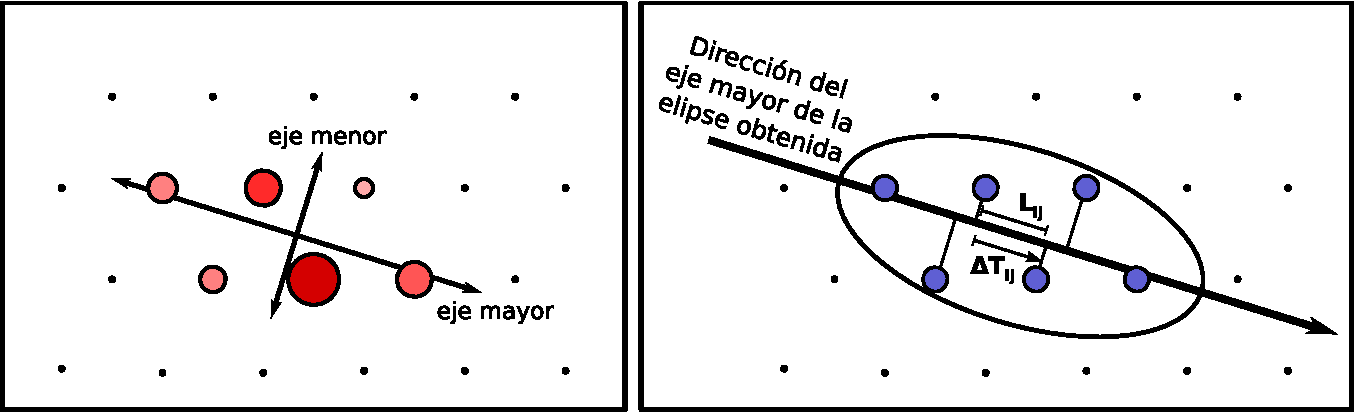
\includegraphics[width=1.0\textwidth]{fig/seleccionAuger/elipse.pdf}
		\caption{Diagrama de la elipse de señal que describe la configuración espacial de un evento inclinado (izquierda). Representación del cálculo de la velocidad de la señal en la dirección del semieje mayor (derecha).}
		\label{fig:elipse}
		\end{center}
		\end{figure}
		%
		
		\subsection{Eventos de 3 estaciones en ES}
		\label{sbsc:3StIncl}
		
		Los eventos de 3 estaciones presentan una incerteza elevadae n la reconstrucción\footnote{Si se la compara con la performance alcanzada por los eventos de más estaciones.}, por lo que es más probable que sean clasificados como inclinados cuando no lo son.
		Tanto es así, que en las búsquedas de DG se los descarta.
		En cambio, dado que en la búsqueda de ES estos representan alrededor del 30$\%$ de la muestra de señal\footnote{Que como se ver\'a m\'as adelante, es alrededor de 5 veces la importancia del canal DGL.}, se decidi\'o incluirlos aunque aplic\'andoles un tratamiento diferencial.
		Esto implica un criterio especial al clasificarlos como inclinados y como jóvenes.
		
		Hay sólo 7 configuraciones de 3 estaciones que satisfacen los requisitos de trigger T3, que se muestran en la figura \ref{fig:3stConf}.
		Gracias a que este número es manejable, además de aplicar cortes en las variables presentadas hasta el momento, se agregará un requisito adicional sobre el tipo configuración de estos eventos.
		La idea es conservar las propensas a aparecer en la muestra de señal mientras se eliminan las que proclives a inducir candidatos falsos.
		%
		\begin{figure}[ht!]
		\begin{center}
		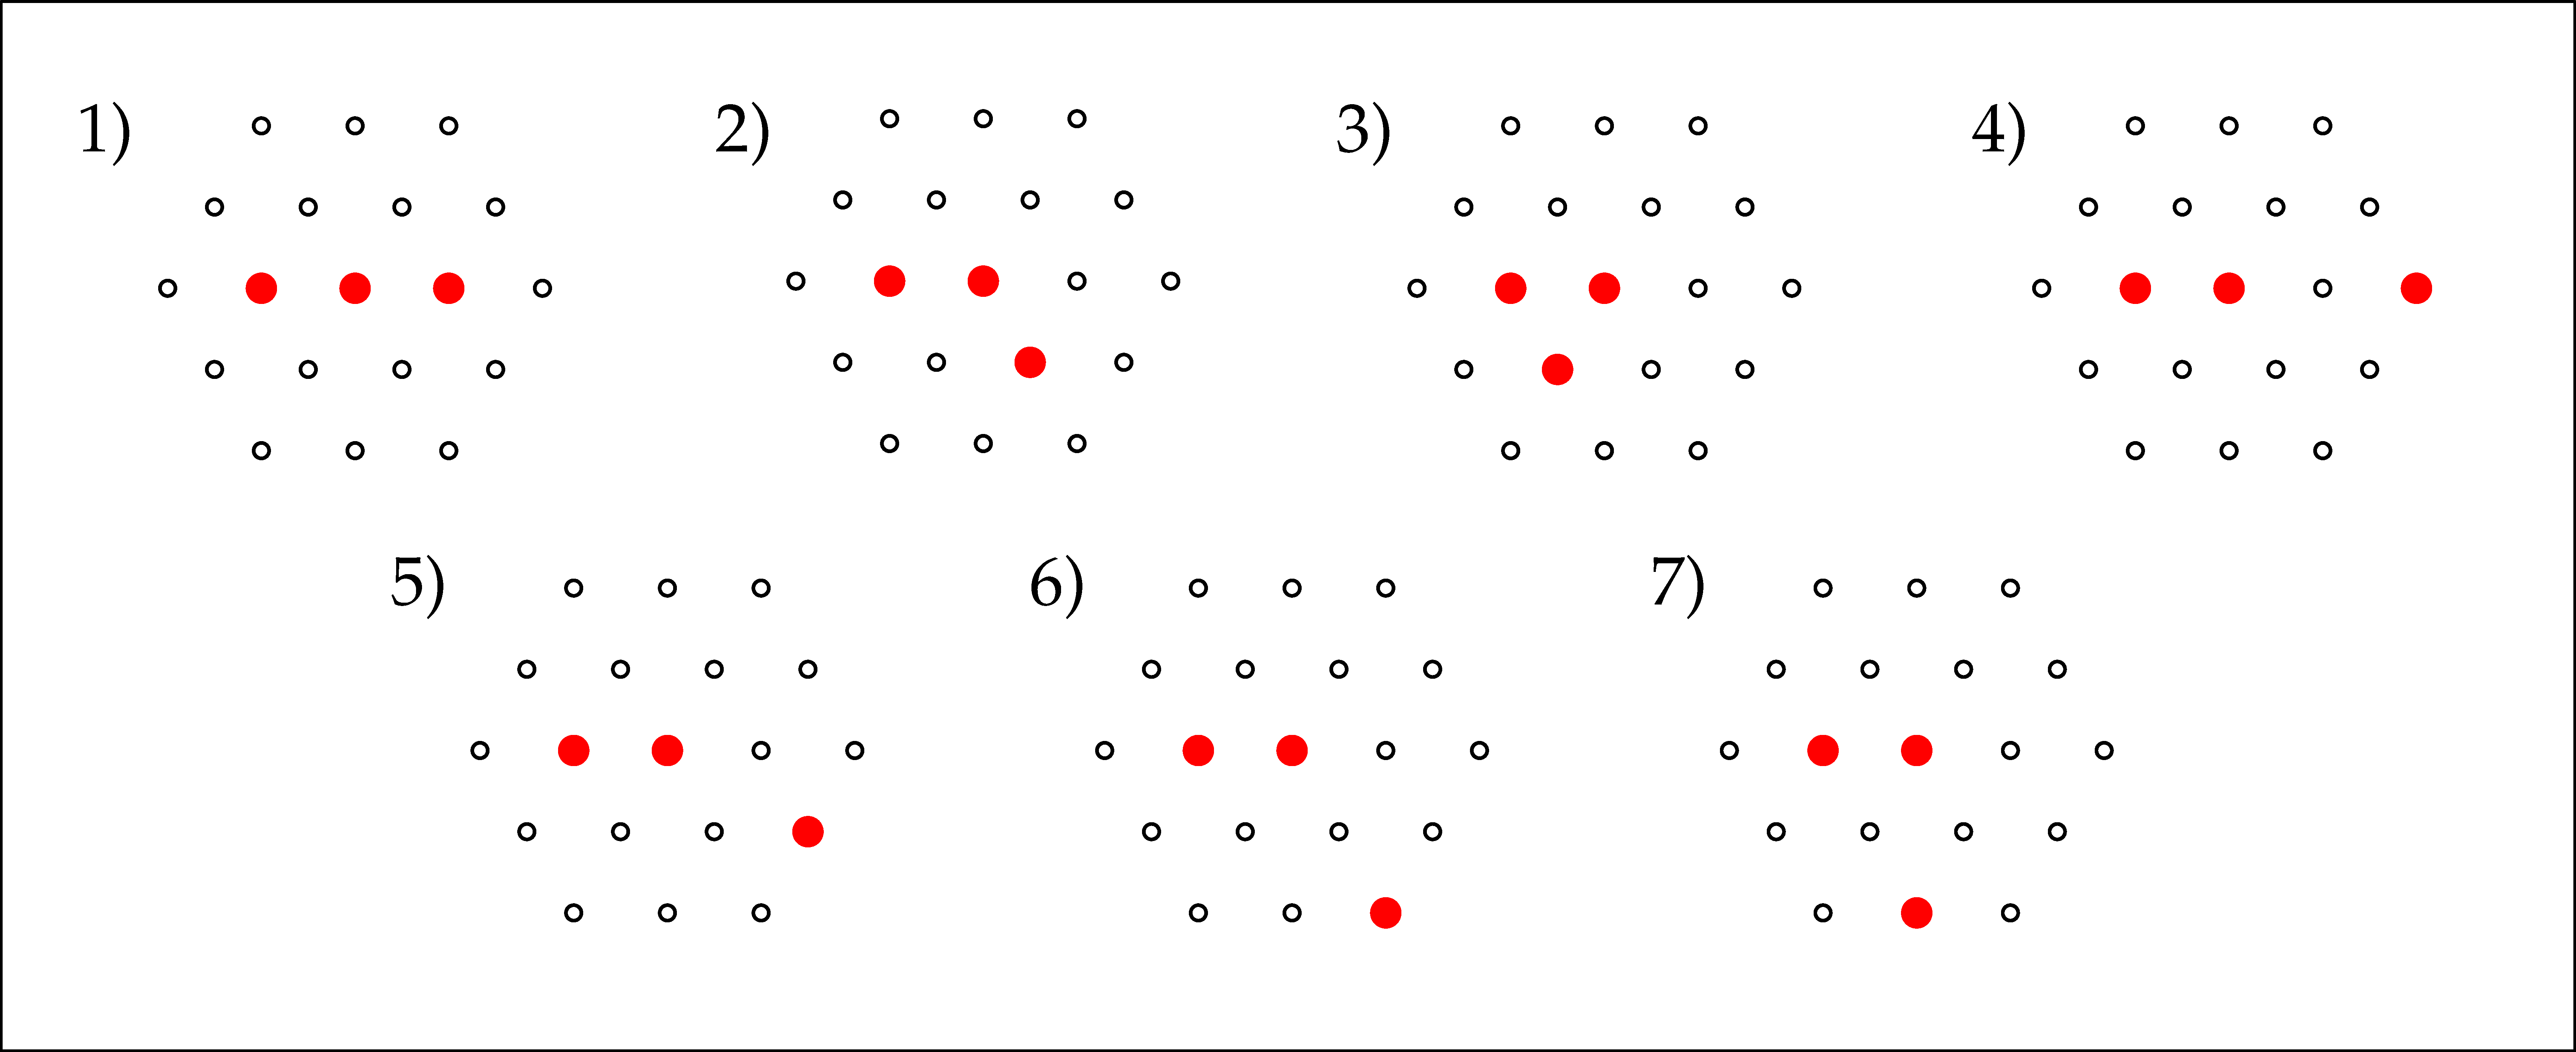
\includegraphics[width=1.0\textwidth]{fig/seleccionAuger/3stConf}
		\caption{Bosquejo de las 7 posibles configuraciones de 3 estaciones que pueden lograr disparo T3. Cabe destacar que cada estación debe haber disparado con nivel ToT.}
		\label{fig:3stConf}
		\end{center}
		\end{figure}
		%
		En la tabla \ref{tab:3stConf} muestra la frecuencia de aparición en el MC de neutrinos ES luego de aplicar los criterios de calidad.
		%
		\begin{table}[!h]
		\centering
		\begin{tabular}{|c|c|c|c|c|}
		\hline
		Config. & MC Events & $\%$ & $\%$ Pesado & Datos                  \\
		\hline
		Total & 3562 & 100\% & 100\%& 10329\\
		\hline
		1 & 1993 & 56.0\% & 70.8\% & 1378\\
		2 & 132 & 3.7\% & 0.5\% & 1895\\
		3 & 3 & $<$0.1\% & $<$0.1\% & 6358\\
		4 & 142 & 4.0\% & 1.8\% & 82\\
		5 & 1278 & 35.9\% & 26.9\% & 378\\
		6 & 8 & 0.2\% & $<$0.1\% & 38\\
		7 & 9 & 0.2\% & $<$0.1\% & 200\\
		\hline
		\end{tabular}
		\caption{
		\label{tab:3stConf}
		Frecuencia de aparición de las distintas configuraciones mostradas en la figura \ref{fig:3stConf} luego de aplicar los criterios de calidad.
		Se muestran, de la columna 2 a 4 la cantidad de eventos MC en cada configuración, porcentaje de aparición y su porcentaje pesado.
		La última columna presenta el número de eventos en la muestra de fondo para cada configuración.
		}
		\end{table}
		%
		En la muestra de señal, compuesta por eventos muy inclinados, las dos configuraciones dominantes son la 1 y la 5. Las razones por las que el resto de configuraciones no son frecuentes son las siguientes:
		\begin{itemize}
		 \item Las configuraciones 2 y 3 son demasiado compactas y anchas. Los neutrinos ES típicamente dejan huellas muy alargadas. Si un evento ES tuviera el ancho suficiente para disparar esas tres estaciones, usualmente dispararía algunas más, generando un evento de mayor multiplicidad.
		 \item Las configuraciones 6 y 7 son improbables dado que en el caso de haber una estacion dentro del triángulo formado por las tres estaciones disparadas, tambien sería disparada.
		 \item La configuración 4 es la tercera en abundancia. Esto es rasonable debido a que es una configuración bastante alineada, típica de neutrinos ES. Sin embargo, se encuentra desfavorecida ya que requiere una estación intermedia no disparada.
		\end{itemize}
		
		Si el objetivo de obtener una eficiencia alta a neutrinos ES, no se gana mucho conservando las configuraciones 2, 3, 4, 6 y 7. Por este motivo, siendo conservador, se las descarta.
		En cambio, la configuración 1 además de ser frecuente es compacta, por lo que debe ser conservada.
		Finalmente, dado que hasta el momento Auger no ha detectado ningun neutrino, se consideró que un evento candidato que presente la configuración 5 daría lugar a escepticismo de parte de la comunidad. Por todo esto, en la búsqueda de neutrinos ES, sólo se aceptan eventos de 3 estaciones de configuración 1.
		
		\subsection{Desempeño de la selección de eventos inclinados}
		
		Finalmente, la selección de eventos inclinados se realiza en cada análisis utilizando los cortes que aparecen en la tabla \ref{tab:inclSel}.
		Estos cortes fueron definidos en base a un compromiso entre conseguir alta eficiencia de selección de neutrinos y baja aceptación de eventos poco inclinados.
		%
		\begin{table}[ht!]
		\begin{center}
			\renewcommand{\arraystretch}{1.4}
			\scriptsize
			\begin{tabular}{|l|c|c|c|}
			\hline
			Búsqueda & Earth-skimming (ES)           & Downward-going                        & Downward-going                       \\
					&                               & {\it high} angle (DGH)                & {\it low} angle (DGL)                \\
			\hline
						& $-$                             & $\theta_{\rm rec}>$ 75$^{\circ}$   &   $\theta_{\rm rec}\in (58.5^\circ,~76.5^{\circ})$\\
			Lluvias    & $L/W > 5$                                         & $L/W > 3$ & $-$ \\
			Inclinadas & $\langle V\rangle\in (0.29,~0.31)~{\rm m~ns^{-1}}$ & $\langle V \rangle~<~0.313~{\rm m~ns^{-1}}$ & $-$ \\
					& RMS($V$)$~<~0.08~{\rm m~ns^{-1}}$                 & RMS($V$)/$\langle V\rangle<0.08$ & $-$ \\
					& Conf 1 si $N_{ST}=3$ & & \\
			\hline
			Efficiencia & \multicolumn{3}{c|}{$\sim90\%$}\\
			\hline
			\end{tabular}
			\vskip -3mm
			\caption{Resumen de los observables y valores numéricos de los cortes aplicados para seleccionar lluvias inclinadas en las tres búsquedas de neutrinos.} 
		\end{center}

		\label{tab:inclSel}
		\end{table}
		%
		Como factor extra se procur\'o que, dado que la muestra de fondo consiste en una fracción de los datos del detector, luego de la selección quede una cantidad suficiente de eventos en la muestra de entrenamiento que permita definir el criterio de selección de lluvias jóvenes.
		
		En los tres análisis la eficiencia de selección de lluvias inclinadas para la muestra de señal alcanz\'o valores cercanos al $90\%$, pesados según lo que se expuso en la sección \ref{sc:pesos}.
		
\section{Selecci\'on de lluvias j\'ovenes}
\label{sc:selNu}
	
	Una vez aplicadas a las muestras de fondo y señal las selecciones de eventos de calidad y de lluvias inclinadas, se definió la selección de lluvias jóvenes mediante el método iterativo que se esquematiza en la figura \ref{fig:entrenamiento},
	%
	\begin{figure}[ht!]
		\begin{center}
		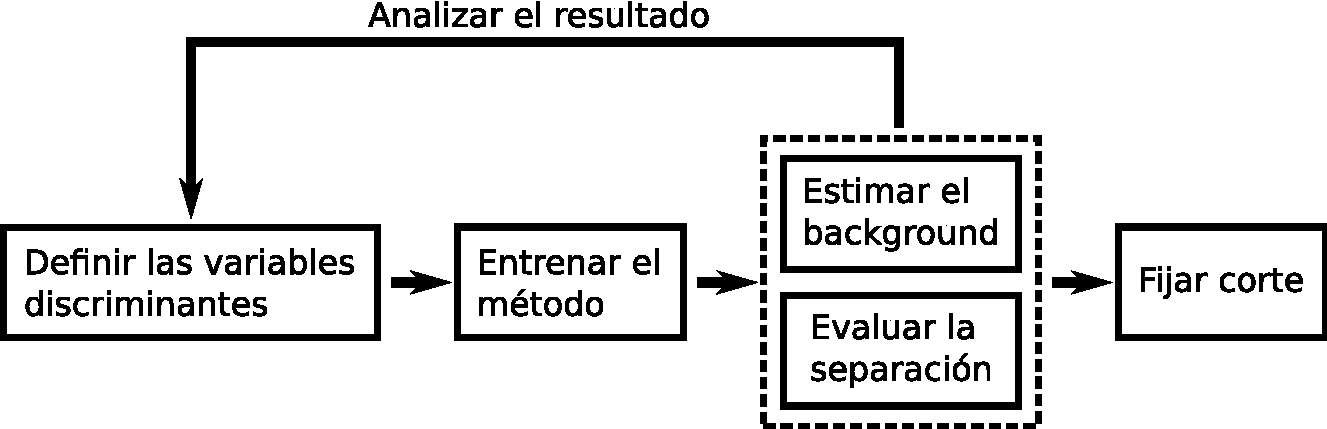
\includegraphics[width=1.0\textwidth]{fig/seleccionAuger/entrenamiento}
		\caption{Diagrama de flujo del método utilizado para definir la selección de lluvias jóvens en los tres análisis.}
		\label{fig:entrenamiento}
		\end{center}
	\end{figure}
	%
	que cuenta con tres pasos claramente definidos:
	\begin{enumerate}
	 \item \textbf{Definición de variables discriminantes}: consiste en definir mediante argumentos físicos variables que contengan información sobre si un evento pertenece a la muestra de señal o a la muestra de fondo.
	 \item \textbf{Entrenamiento del método}: en esta etapa se extrae la información de las variables para definir un posible criterio de selección. 
	 \item \textbf{Estimación de la eficiencia y la contaminación}: se eval\'ua el desempe\~no del criterio preeliminar definido en el punto anterior. Si la separación entre muestras es buena, y la probabilidad de obtener eventos espúreos debidos al fondo es aceptable se aprueba el método. Caso contrario se vuelve al paso 1 y se modifica el conjunto de variables discriminantes.
	\end{enumerate}
	%
	\subsection{Variables discriminantes}
	\label{sbsc:discVars}
	
	En el capitulo \ref{sc:easNu} se argumentó que las lluvias hadrónicas inclinadas se inician en el tope de la atmósfera y sólo su componente muónica alcanza el detector.
	En cambio, las provocadas por neutrinos tienen la posibilidad de interactuar cerca de la superficie, lo que permite una cantidad significativa de componente electromagnética (EM) a nivel del suelo.
	En los eventos DG la componente EM se concentra en la región del detector sobre la que la lluvia interactúa primero, o regi\'on temprana del evento.
	Sin embargo, en los eventos iniciados por neutrinos ES la evolución hacia arriba del evento permite que la componente EM alcance la mayor parte de las estaciones que se disparen y no sólo las de la zona temprana.
	Esto se ilustra en la figura \ref{fig:compNus} en la que se representan las componentes muónica y electromagnética de una lluvia hadrónica típica, de un neutrino DG y de uno ES.
	%
	\begin{figure}[ht!]
		\begin{center}
		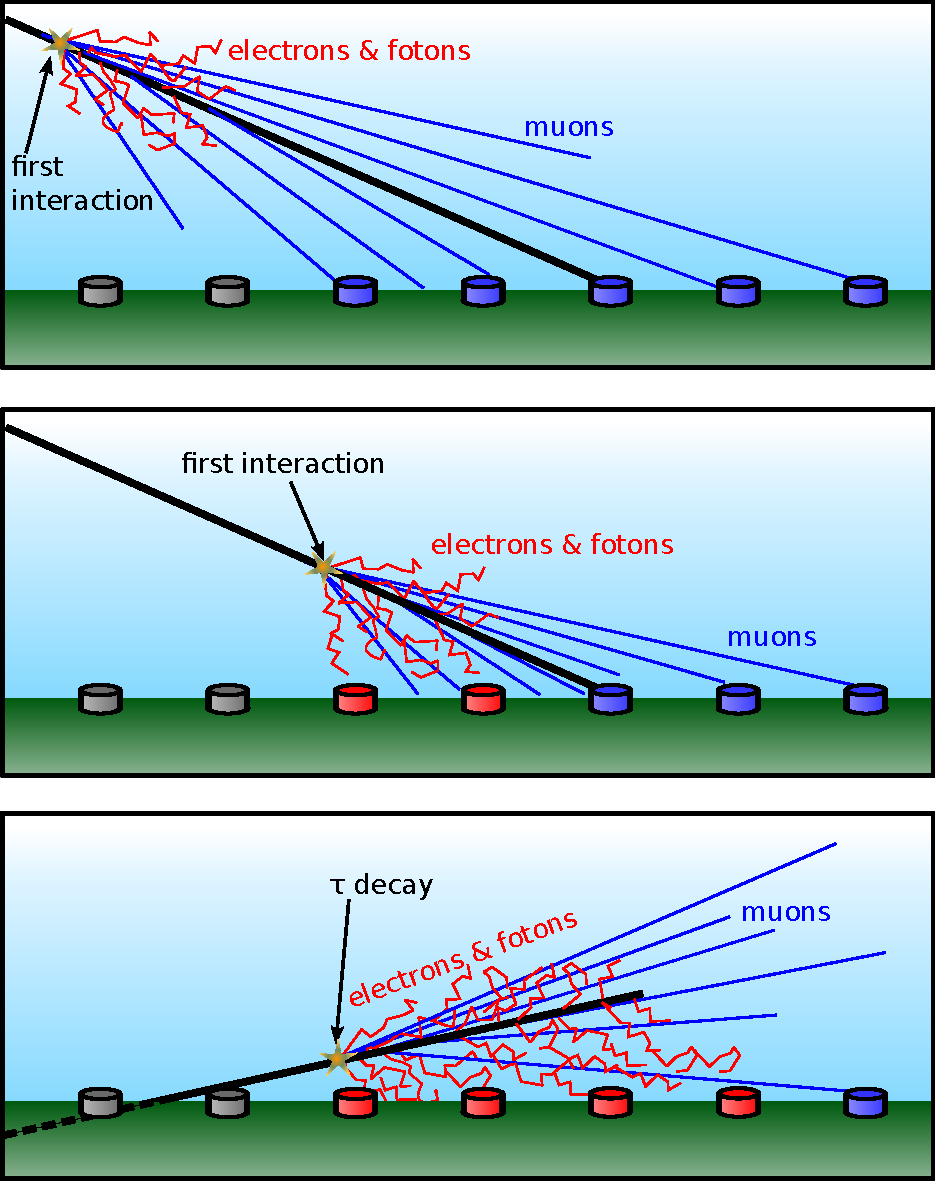
\includegraphics[width=0.7\textwidth]{fig/seleccionAuger/inclined_regular_dg_and_up}
		\caption{Arriba: Esquema de una lluvia inclinada iniciada por un hadrón que interactúa alto en la atmósfera. Medio: Lluvia profunda iniciada por un neutrino DG. La parte temprana del evento presenta una señal electromagnética significativa. Abajo: evento iniciado por un \tauon{} que emerge de la tierra producto de un neutrino ES. La componente electromagnética puede alcanzar todas sus estaciones.}
		\label{fig:compNus}
		\end{center}
	\end{figure}
	%
	
	Entonces fue necesario conseguir variables del detector que sean sensibles a la precencia de componente electromagnética.
	Esta, usualmente provoca señales en el SD cuya duración puede alcanzar algunos cientos de nano segundos, mientras que las señales generadas por la componente muónica no suele superar la centena.
	Entonces, a partir de las trazas FADC es posible construir observables correlacionados con la estructura temporal de la señal y analizar su desempeño.
	A continuación se definen algunos que fueron evaluados como posibles:
	\begin{itemize}
	 \item \textbf{Numero de estaciones con trigger ToT:} como se discutió en la sección \ref{sbsc:trig_levels}, el triger ToT fue ideado para detectar señales extendidas en el tiempo.
	 Por ello, un observable sensible a la señal electromagnética en un dado evento podría ser la cantidad de estaciones con este nivel de trigger.
	 El problema con esta variable es que, al ser discreta dificulta cualquier estimación de fondo.
	 \item \textbf{RT/FT:} Se llama Rise Time (RT) y Fall Time (FT) al tiempo que le toma a la señal alcanzar desde el $10\%$ de su integral hasta el $50\%$ y desde el $50\%$ hasta el $90\%$ respectivamente.
	 Estas poseen al ventaja de que son una medida directa del observable que nos interesa, la duración de la señal, por lo que ambas variables muestran poder de discriminación entre la muestra de señal y de fondo (ver figura \ref{fig:directObs}).
	 Por otro lado, la precencia de \emph{outliers} en la muestra de fondo dificulta el control de la contaminación.
	 Este tipo de señales, aunque poco frecuentes, son inaceptables en una busqueda de señal esperada tan pequeña como es la de neutrinos.
	 %
	 \begin{figure}[ht!]
		\begin{center}
		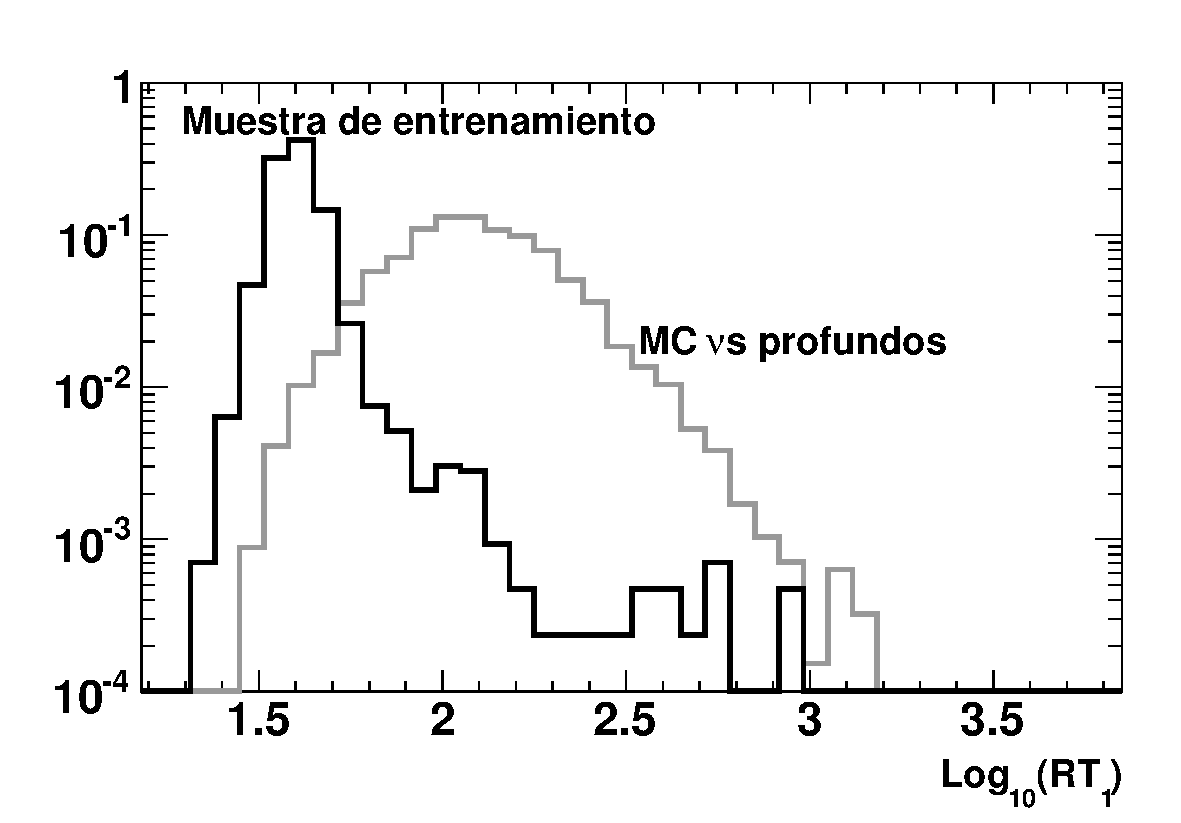
\includegraphics[width=0.48\textwidth]{fig/seleccionAuger/rt1}
		\hfill
		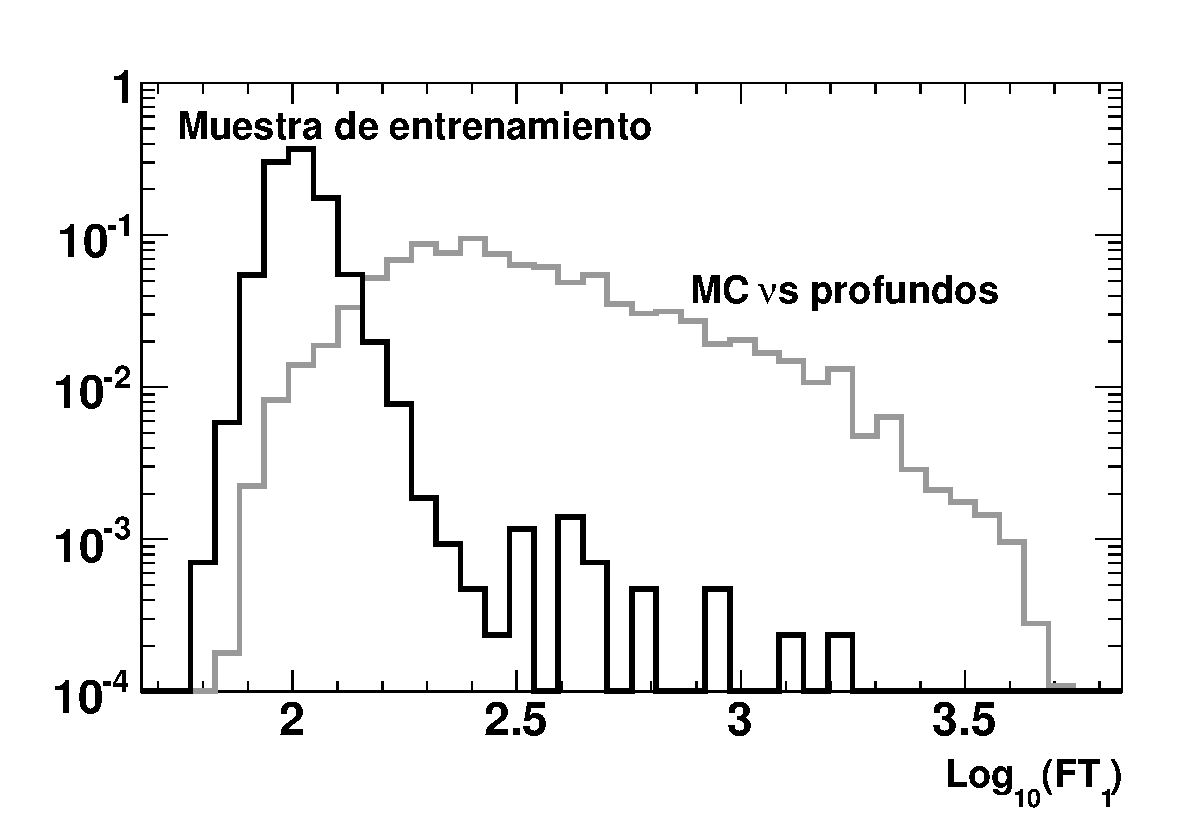
\includegraphics[width=0.48\textwidth]{fig/seleccionAuger/ft1}
		\\
		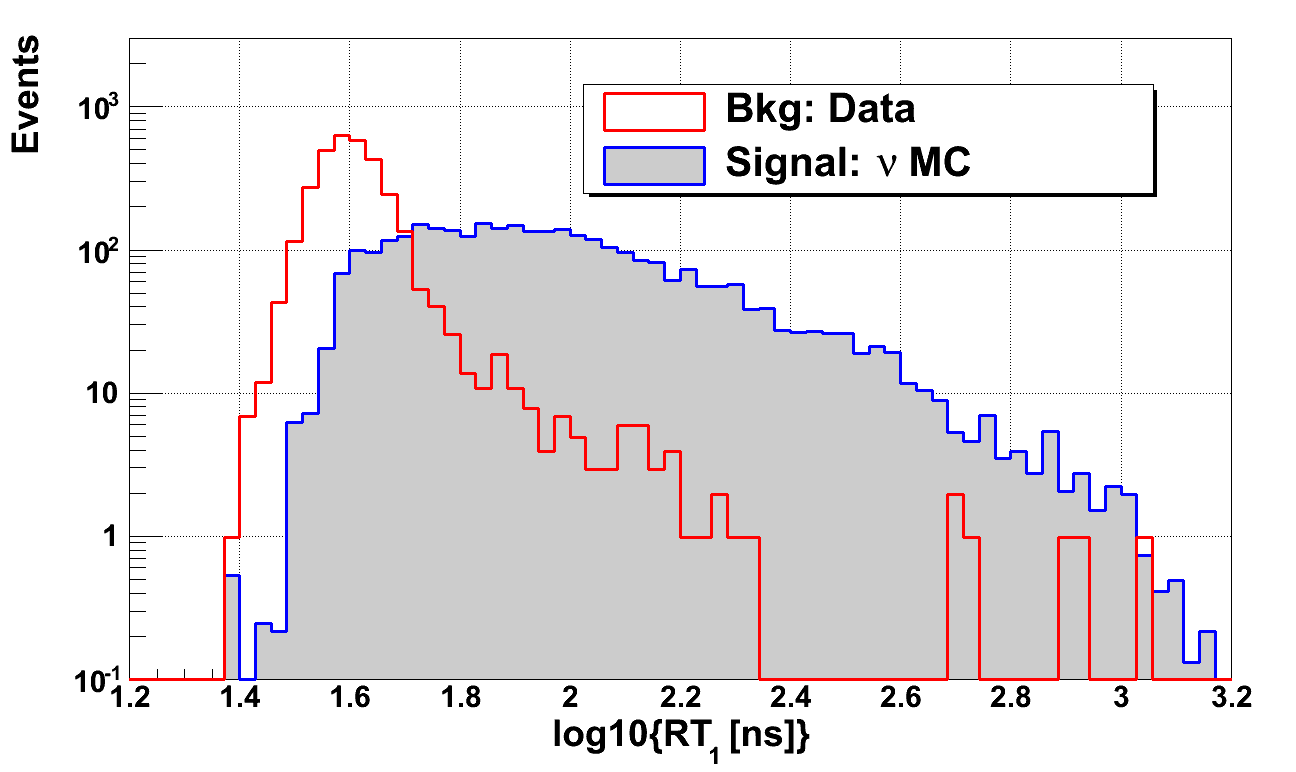
\includegraphics[width=0.48\textwidth]{fig/seleccionAuger/rt_forThesis}
		\hfill
		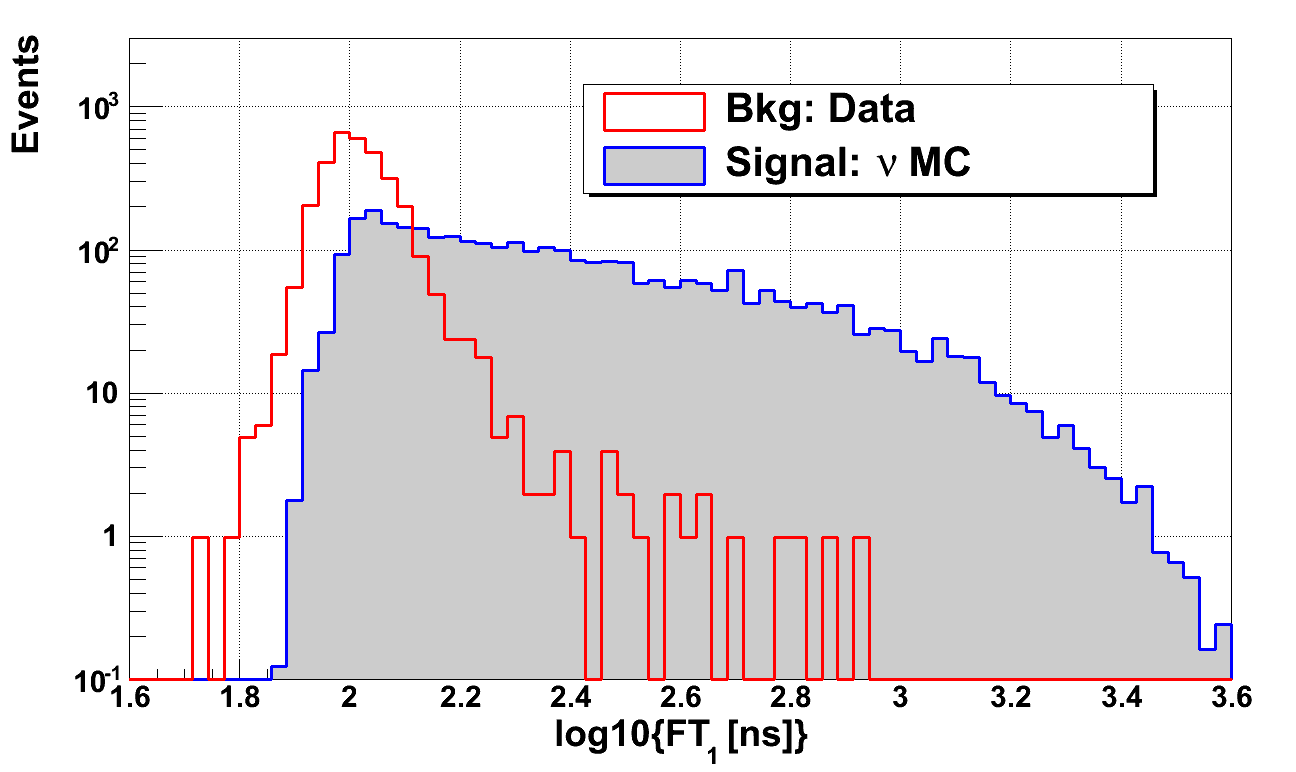
\includegraphics[width=0.48\textwidth]{fig/seleccionAuger/ft_forThesis}
		\caption{Distribuciones de $\log RT$ y $\log FT$, arriba para eventos DGH y abajo para eventos ES. Si bien en ambos casos se evidencia separación entre las muestras, la aparición de \emph{outliers} dificulta el control de la contaminación debido al fondo.}
		\label{fig:directObs}
		\end{center}
	\end{figure}
	 %
	 \item \textbf{AoP:} se llama AoP, o Area Over Peak, a la la integral de la FADC (su área) dividida por el máximo valor que haya alcanzado, como se muestra en la figura \ref{fig:aopDef}.
	 %
	 \begin{figure}[ht!]
		\begin{center}
		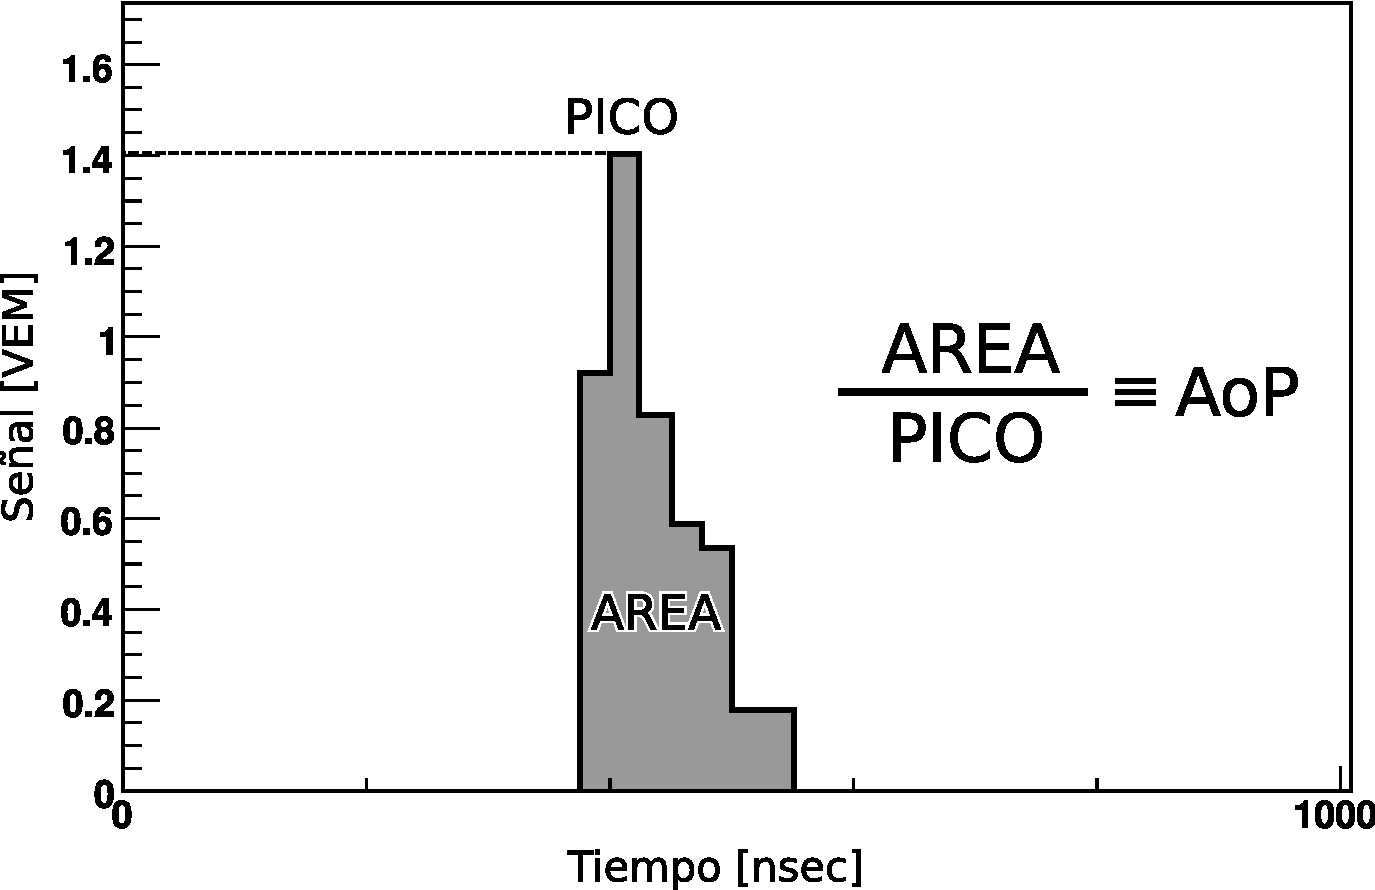
\includegraphics[width=0.6\textwidth]{fig/seleccionAuger/AoP_def}
		\caption{Definición de la variable AoP. Esta consiste en la integral de la FADC dividida por el máximo valor que esta haya alcanzado. Esta variable toma valores cercanos a uno para señales muónicas y mayores para electromagnéticas.}
		\label{fig:aopDef}
		\end{center}
	 \end{figure}
	 %
	 Esta variable se calibra para que los muones verticales tengan un valor medio de AoP$=1$.
	 En cambio, las señales cuyo origen es la componente EM de la lluvia presentan valores mucho mayores, como se observa en la figura \ref{fig:aopDist}.
	 %
	 \begin{figure}[ht!]
		\begin{center}
		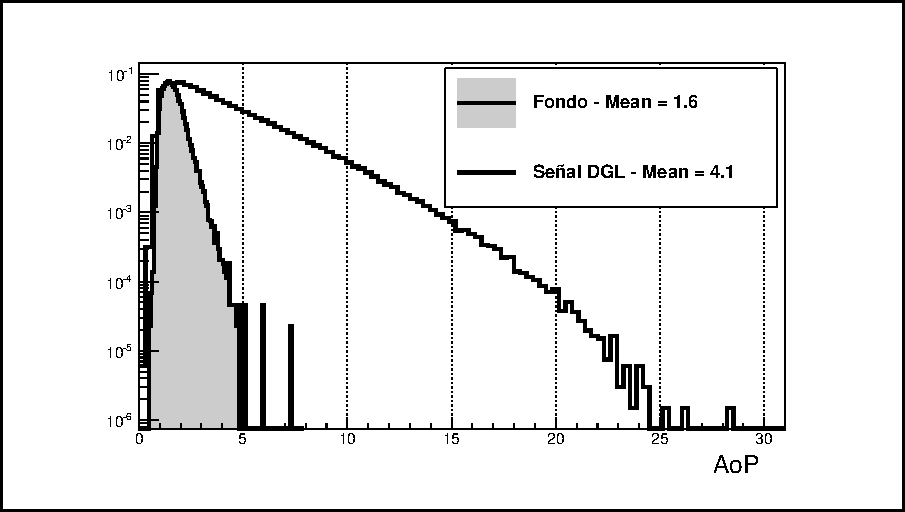
\includegraphics[width=0.6\textwidth]{fig/seleccionAuger/aopDGL} \\
		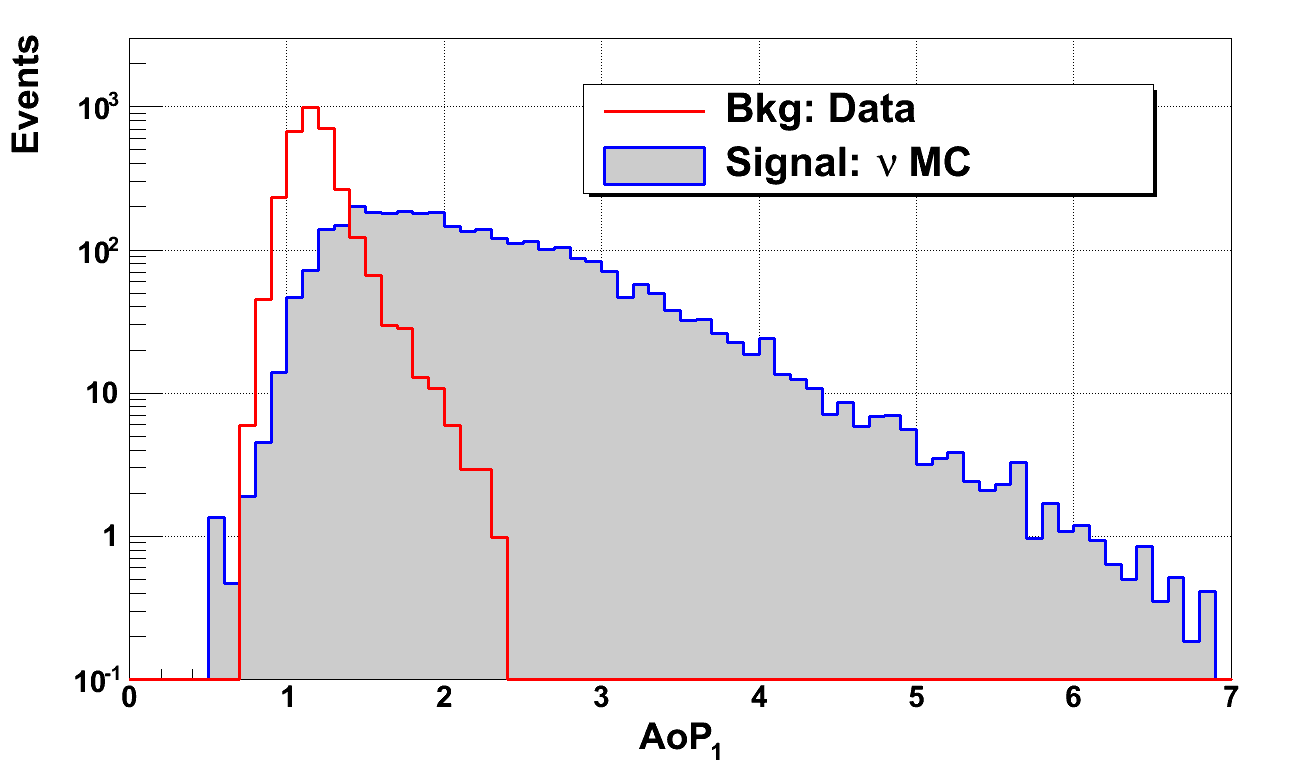
\includegraphics[width=0.6\textwidth]{fig/seleccionAuger/aop_forThesis}
		\caption{Distribuciones de la variable AoP para señál y fondo. Arriba para neutrinos DGL y abajo para eventos ES. En ambos casos los eventos inclinados de la muestra de fondo presentan valores cercanos a 1 mientras que el valor medio para las muetras de señal es mayor.}
		\label{fig:aopDist}
		\end{center}
	 \end{figure}
	 %
	 Además de buena separación, esta variable no presenta colas largas en la muestra de fondo, por lo que el control de la contaminación se ve favorecido.
	\end{itemize}
	
	Las variables definidas hasta el momento se calculan de manera local, es decir, para cada estación.
	Para extraer la mayor cantidad de información posible, es necesario utilizar variables globales, que además de la información local, incluyan correlaciones entre las variables en distintas estaciones.
	A continuación se detallan las variables estudiadas en los distintos análisis.
	
	\subsubsection{ToTF}
	La variable \emph{ToT fraction} ToTF se define como la fracción de estaciones del evento que dispararon con trigger ToT y además poseen un valor de AoP$\geq1.4$.
	La distribución de esta variable se muestra en la figura \ref{fig:totfDist}.
	%
	\begin{figure}[ht!]
		\begin{center}
		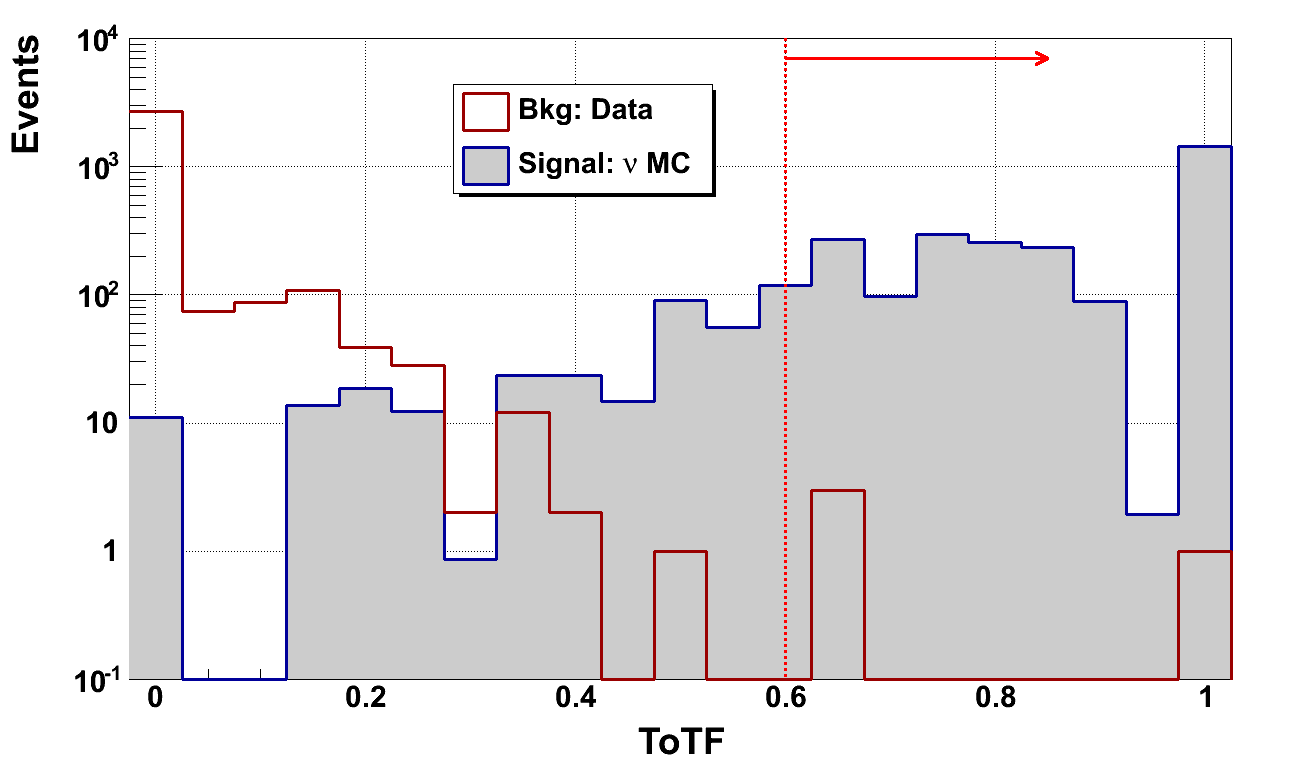
\includegraphics[width=0.6\textwidth]{fig/seleccionAuger/ToTF_forThesis}
		\caption{Distribuciones de la variable ToTF para señal y fondo. Si bien la separación exhibida entre las muestras es notable, la posibilidad de estimación de la contaminación se ve desfavorecida.}
		\label{fig:totfDist}
		\end{center}
	\end{figure}
	%
	Si bien la separación exhibida entre las muestras es notable, la posibilidad de estimación de la contaminación se vuelve extremadamente dificil.
	
	\subsubsection{Variables derivadas de AoP}
	
	Para analizar la evolución de la variable AoP a lo largo del evento, resulta útil observar su promedio según el órden de disparo de las estaciones dentro del evento, lo que se grafica en la figura \ref{fig:aop_vs_NStation} para eventos de seis estaciones.
	%
	\begin{figure}[ht!]
		\begin{center}
		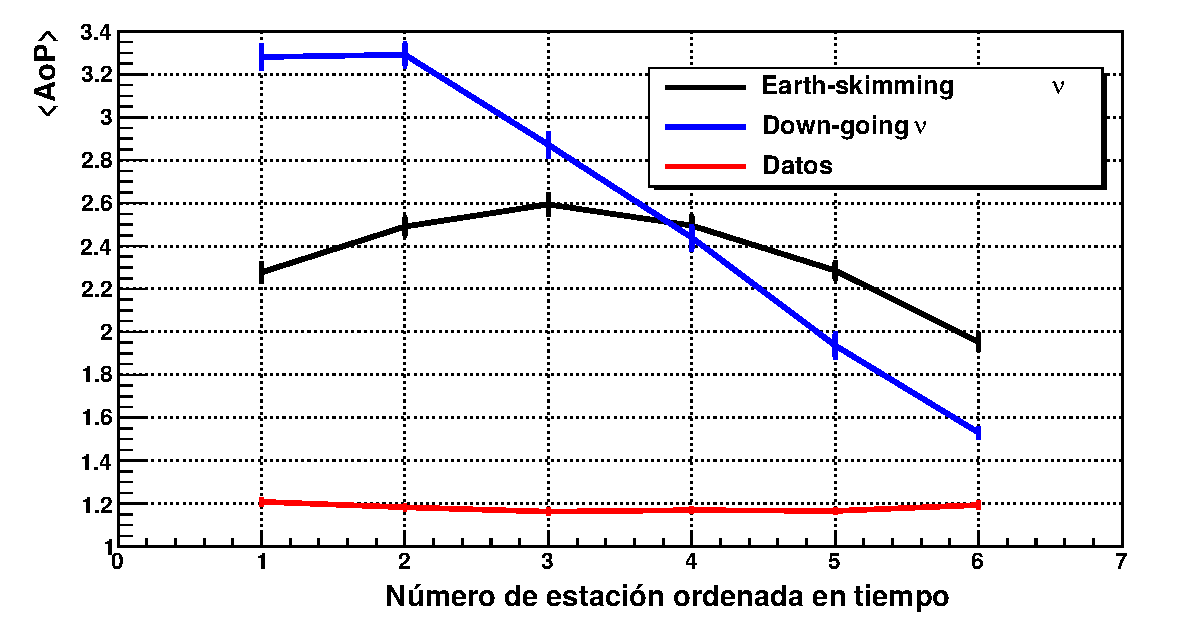
\includegraphics[width=0.8\textwidth]{fig/seleccionAuger/aop_vs_NStation}
		\caption{Promedio de AoP en función del número de la estación. Este se asigna según el órden de disparo dentro de cada evento. Se observa que los eventos DG presentan mayor diferencia en las estaciones tempranas, mientras que en los eventos ES esta se mantiene a lo largo de todo el evento.}
		\label{fig:aop_vs_NStation}
		\end{center}
	\end{figure}
	%
	Como se hab\'ia adelantado, se observa que los eventos DG presentan mayor separación en las estaciones más tempranas de los eventos, mientras que en las lluvias ES esta se mantiene a lo largo de todos los tanques\footnote{Este comportamiento se observa en eventos de todas las multiplicidades.}. 	
	Teniendo todo esto en cuenta se consideraron tres tipos de variables:
	\begin{enumerate}
	 \item \textbf{Producto de AoPs:} por las razones ya expuestas, se espera que las lluvias inclinadas presenten valores de AoP elevados. Así, su producto es una medida de esta característica global del evento. Una de las ventajas de esta variable discriminante es que es muy estable frente a fluctuaciones que puedan sufrir las estaciones individuales (ver panel superior izquierdo en la figura \ref{fig:observablesGlobales}). 
	 \item \textbf{Promedio de AoPs:} del mismo modo, el AoP promediado sobre todas las estaciones es otra variable prometedora que posee las mismas bondades que la anterior (ver panel superior derecho en la figura \ref{fig:observablesGlobales}).
	 \item \textbf{Asimetría:} en el caso de las lluvias DG, la diferencia entre las AoPs promediadas sobre las primeras  y las últimas estaciones de un evento puede ser otra variable con poder discriminante (ver panel inferior en la figura \ref{fig:observablesGlobales}). 
	\end{enumerate}
	%
	\begin{figure}
	\begin{center}
	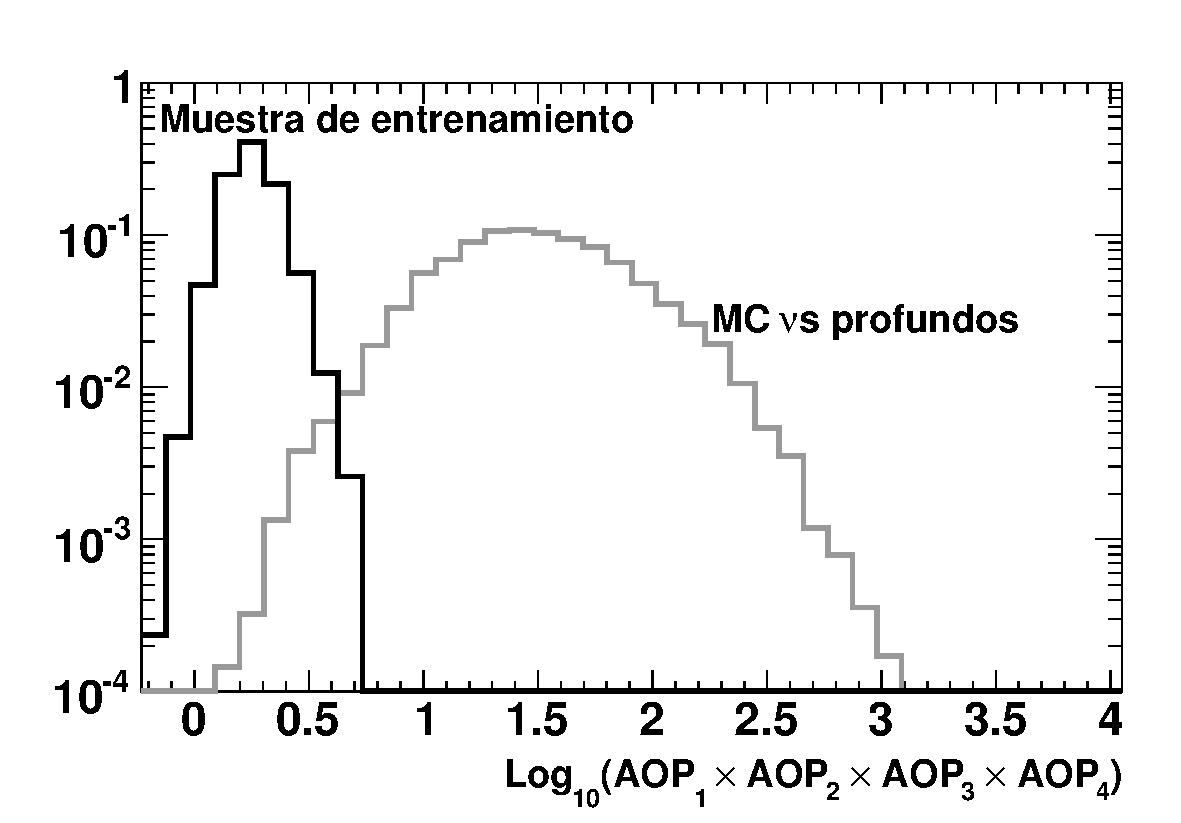
\includegraphics[width=0.47\textwidth]{fig/seleccionAuger/aop_prod.pdf} \hfill
	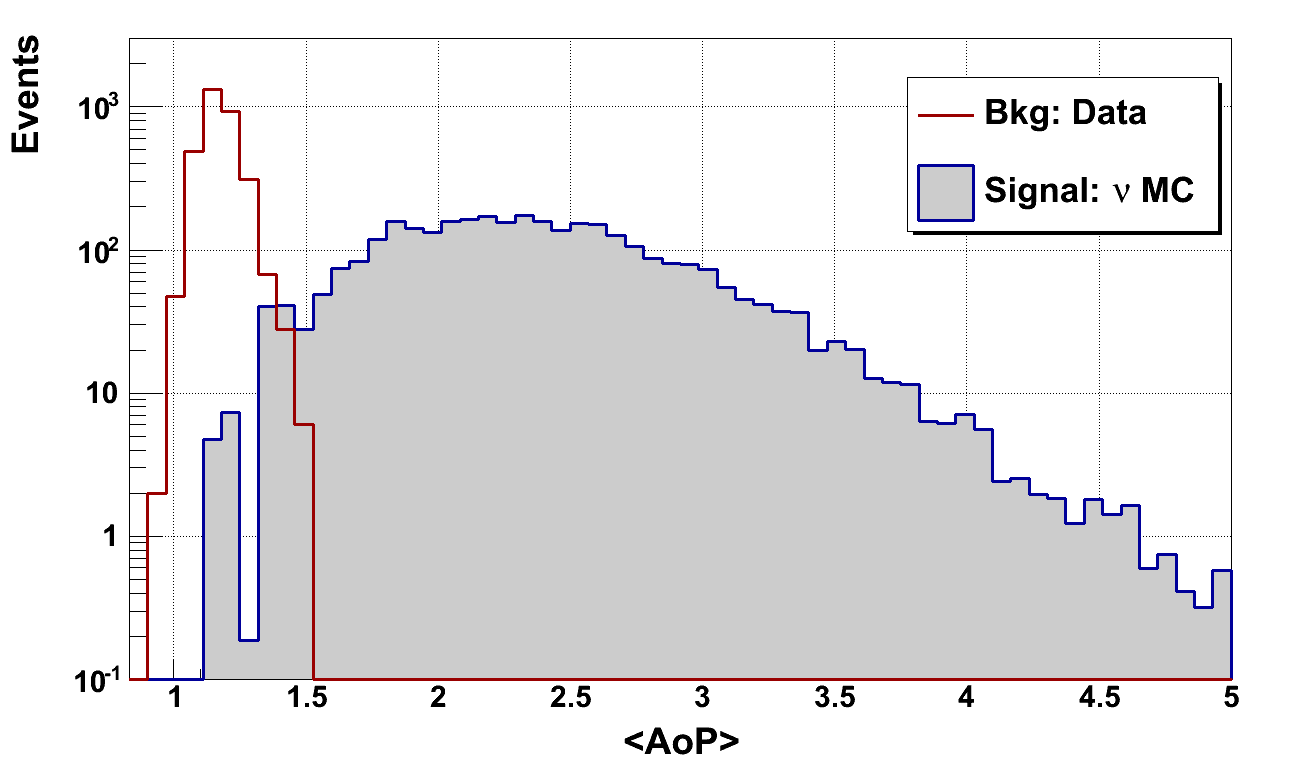
\includegraphics[width=0.47\textwidth]{fig/seleccionAuger/trainning_withMCSimple_log_forThesis}\\
	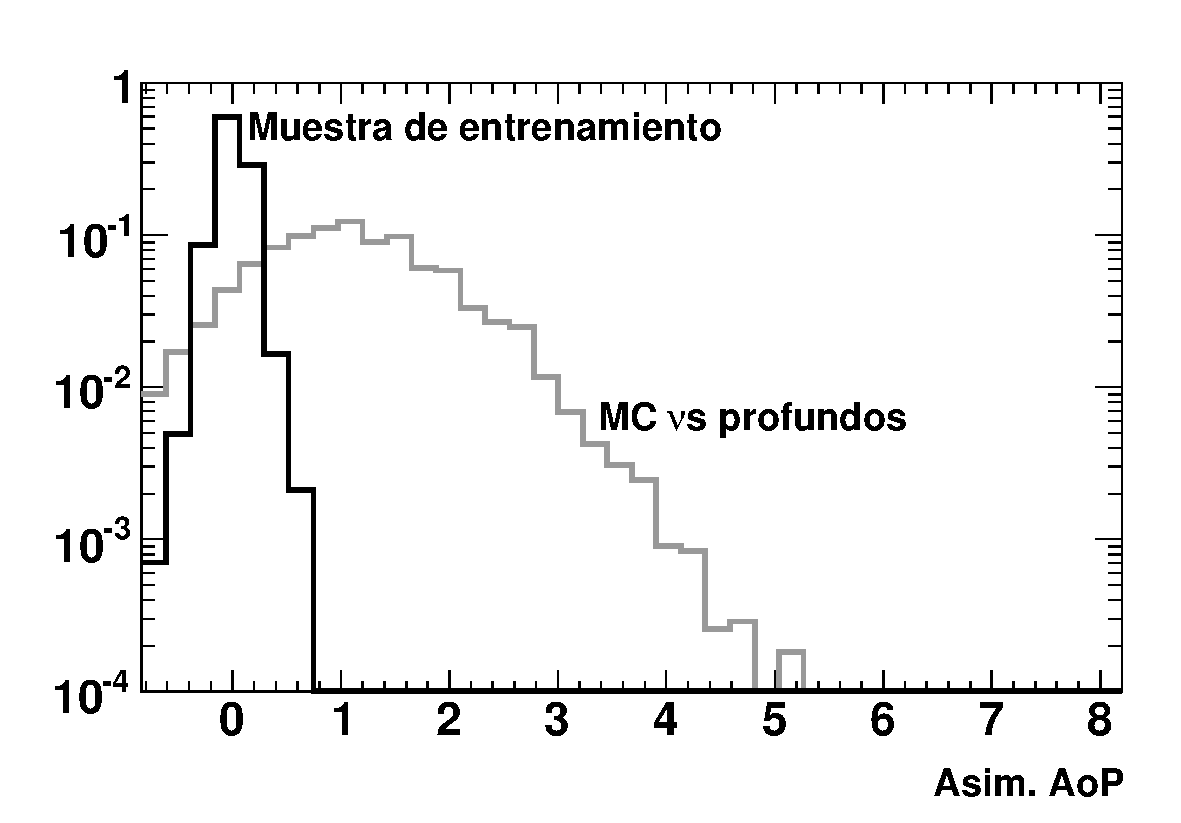
\includegraphics[width=0.47\textwidth]{fig/seleccionAuger/asim.pdf}
	
	\caption{Distribución de la asimetría del AoP promedio entre estaciones tempranas y tardias (izquierda arriba) y producto del AoP en las cuatro estaciones más tempranas (derecha).}
	\label{fig:observablesGlobales}
	\end{center}
	\end{figure}
	%
% 	\clearpage
	\subsection{Entrenamiento del método}
	
	Una vez definidas las posibles variables discriminantes, es necesario optimizar su conjunto, ejecutando lo que se denomina entrenamiento del método.
	
	La opción más sencilla es aplicar lo que se denominan \emph{cortes cuadrados duros}.
	Este, es un método que consiste en definir una sucesión de variables y fijar sobre ellas cortes que permitan selecciónar a cada paso una fracción (en principio alta) de la muestra de señal.
	La ventaja principal de este método es que es relativamente simple, ya que el conjunto de variables elejidas y cada corte puede comprenderse usualmente mediante argumentos físicos.
	Por otro lado, su principal desventaja es que desperdicia cualquier información guardada en la correlación de las variables.
	
	Para subsanar este inconveniente, es común recurrir a lo que se denominan métodos multivariados o MVA por sus siglas en inglés.
	Estos poseen la ventaja de combinar la mayor parte de la información disponible y obtener así el mayor grado de separación posible, usualmente a costa de esconder la interpretación física del problema.
	Existen en la actualidad una gran variedad de herramientas de este tipo. Entre las más comunmente utilizadas se encuentran: redes neuronales, arboles de decisión y el análisis de componentes principales. 
	Con el objetivo de mantener una interpretación física simple, se en las búsquedas de neutrinos de Auger se decidió adoptar el método de Fisher~\cite{cite:Fisher} para la construcción del algoritmo de identificación.

	La técnica de Fisher forma parte de los métodos de discriminación lineales.
	Partiendo de un conjunto de variables discriminantes construye un nuevo observable ${\cal F}$ como una combinación lineal de ellas.
	Este discriminante es óptimo para el caso de variables gaussianas y, en el caso general, provee la función lineal que brida la mayor separación posible.
	Además, al ser ${\cal F}$ suma de variables aleatoreas, su distribución tiende a ser más gaussiana que la de las variables originales.
	En la figura \ref{fig:ideaFisher} se muestra la idea de funcionamiento del método en un caso particular idealizado.
	%
	\begin{figure}[ht]
	\begin{center}
	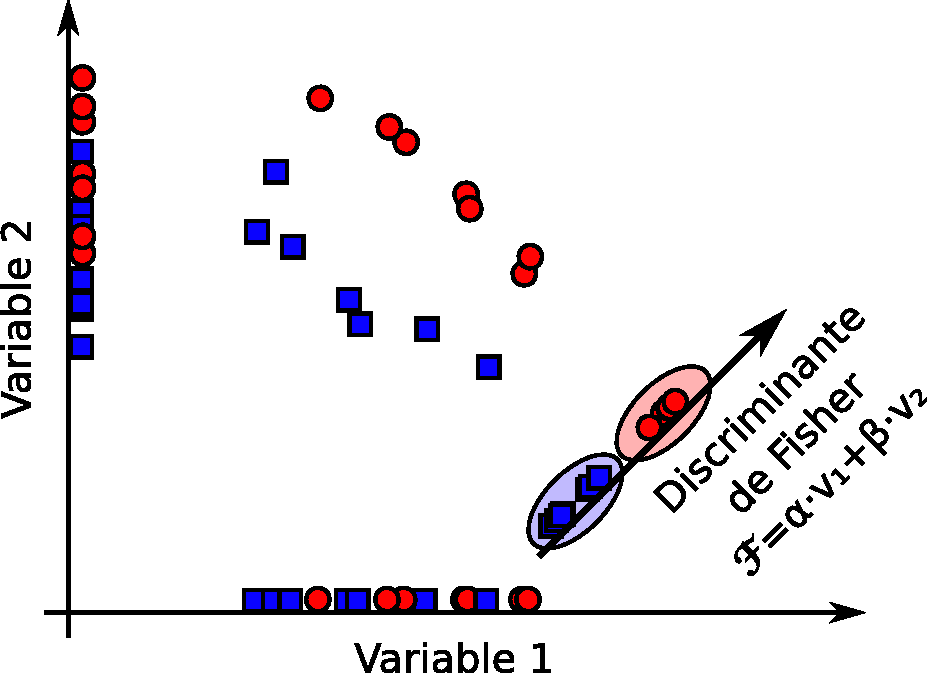
\includegraphics[width=0.75\textwidth]{fig/seleccionAuger/ideaFisher}
	\caption{Esquema de la idea de funcionamiento del método de Fisher. Ninguna de las dos variables originales es capaz de separar las muestras (cuadrados azules y circulos rojos) por si solas. Sin embargo una combinación lineal de ellas logra en este caso una separación completa. El método de Fisher permite obtener las constantes de la combinación lineal óptima (ver texto) a partir de las variables discriminantes provistas.}
	\label{fig:ideaFisher}
	\end{center}
	\end{figure}
	%

	Se define el discriminante de Fisher ${\cal F}$ como:
	%
	\begin{equation}
	{\cal F} = a_1 x_1 + .. + a_n x_n = \vec{a}\cdot \vec{x}
	\end{equation}
	%
	en donde $\vec{a}$ es el vector de los coeficientes de Fisher y $\vec{x}$ un vector que contiene las variables originales.
	Así, puede calcularse la media y la varianza del discriminante usando:
	%
	\begin{eqnarray}
	\langle{\cal F}_X\rangle &=& \vec{a}\cdot\vec{\mu}_X \\
	\text{Var}({\cal F}_X)   &=& \vec{a}^{\,T} \cdot \text{Cov}(X) \cdot\vec{a}
	\end{eqnarray}
	%
	siendo $\vec{\mu}_X$ el vector de valores medios de las variables de la muestra $X$ y Cov$(X)$ su matriz de covarianza.

	A partir de estos ingredientes se construye la función $Q(\vec{a})$ que cuantifica la separación provista por el discriminante $\cal{F}$
	entre las muestras señal y background a la vez que pondera su dispersión:
	%
	\begin{equation}
	Q(\vec{a}) = \frac{( \langle{\cal F}_S\rangle - \langle{\cal F}_B \rangle)^2}{\text{Var}({\cal F}_S)+\text{Var}({\cal F}_B)}
	= \frac{(\vec{a}\cdot\vec{\mu}_S  - \vec{a}\cdot\vec{\mu}_B)^2}
					{\vec{a}^{\,T} \cdot (\text{Cov}(S) + \text{Cov}(B) )\cdot\vec{a}} 
	\end{equation}
	%
	en donde ${\cal F}_S$ y ${\cal F}_B$ representan los valores del discriminante de Fisher para las muestras de señal y fondo respectivamente.
	Al maximizar esta función respecto de los coeficientes $\vec{a}$, se obtiene la combinación lineal de variables que optimiza la separación entre los grupos señal y background a la vez que minimiza sus varianzas manteniendo las distribuciones compactas para evitar la superposición. 
	Estos coeficientes $\vec{a}_{\text{Max}}$ están dados por:
	%
	\begin{equation}
	\vec{a}_{\text{Max}} = (\text{Cov}(S) + \text{Cov}(B) )^{-1} \cdot (\vec{\mu}_S - \vec{\mu}_B)   
	\end{equation}
	
	
	\subsection{Criterio de identificación - Estimación de fondo}
	\label{sbsc:fondo}
	
	Una vez construido el discriminante ${\cal F}$ o definido el conjunto de variables sobre las que se aplican los cortes cuadrados, es posible fijar el corte que separa los eventos hadrónicos de aquellos iniciados por neutrinos.
	Debido a que la señal que se intenta medir es muy pequeña, la sensibilidad del análisis está básicamente limitada por la magnitud de la contaminación esperada.
	Por esto, es fundamental lograr una estimación de la misma y a partir de ella elegir los cortes de selección, buscando siempre que sea lo suficientemente pequeña.
	
	Con esto en mente, una forma de posicionar el corte es de manera tal que se esperen menos de un evento de fondo por encima del mismo cada una cierta cantidad de años $N_{yr}$.
	Para ello, es necesario diseñar un modelo que permita extrapolar la cantidad de eventos esperados para distintos períodos de tiempo.
	Con este fin la estrategia adoptada en los tres análisis fue modelar la cola de la distribución de la muestra de fondo.
	Una vez realizado el ajuste, y teniendo en cuenta que la muestra corresponde a una cantidad conocida de años de datos del detector, es posible renormalizar el modelo a los $N_{yr}$ años (ver  figura\ref{fig:estimaBackground}) para poder calcular la posición del corte.
	%
	\begin{figure}[ht]
	\begin{center}
	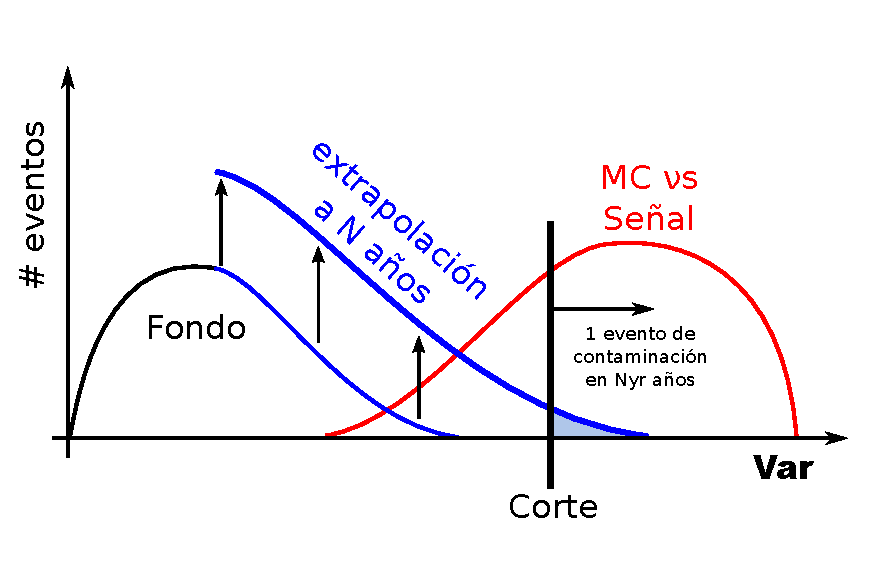
\includegraphics[width=0.8\textwidth]{fig/seleccionAuger/estimaBackground.pdf}
	\caption{Estimación de background debido a eventos hadrónicos que puedan ser erróneamente clasificados como candidatos a neutrinos.}
	\label{fig:estimaBackground}
	\end{center}
	\end{figure}
	%
	
	En este marco, es interesante discutir que el teorema central del límite indica que el discriminante de Fisher, por ser la suma de variables aleatorias, tiende a una distribución gausiana al aumentar el número de términos.
	Sin embargo, debido a que como se verá en las siguientes secciones, la cantidad de variables utilizadas es bajo y además cada una de estas presenta distribuciones asimétricas, no es posible alcanzar un comportamiento gausiano.
	Entonces, para modelar la cola de las distribuciones fue necesario proponer un comportamiento motivado por las características físicas propias del sistema que se analiza.
	
	Debido a que la profundidad de interacción de las lluvias iniciadas por hadrones sigue una distribución exponencial, es esperable que esta característica se vea reflejada de alguna manera en la distribución de las variables discriminantes asociadas a las lluvias más profundas.
	Bajo esta hipótesis en los tres análisis es posible realizar un ajuste exponencial sobre la cola de las distribuciones de fondo en la región $[1\sigma, 3\sigma]$ (con esta notación denominamos al intervalo $[\mu+1\sigma, \mu+3\sigma]$, donde $\mu$ y $\sigma$ son la media y el RMS de la distribución de fondo) y extrapolar el comportamiento.
	Luego, con el fin de evaluar la bondad del ajuste, es posible utilizar las regiones de $[3\sigma, 4\sigma]$, $[4\sigma, 5\sigma]$ y $[5\sigma, 6\sigma]$, calculando en cada una la cantidad de eventos predichos por el ajuste con lo observado.
	Si los resultados son compatibles se renormaliza la distribución a $N_{yr}$ y se coloca el corte tal que se espere un evento por encima del mismo.
	Asimismo, una vez el corte se encuentra definido es posible también evaluar la eficiencia de selección de neutrinos.
	Si se obtiene un buen nivel de predicción en las zonas de $[3\sigma, 6\sigma]$ y el nivel de eficiencia es aceptable, se acepta el criterio de selección.
	En caso contrario, se debe realizar el procedimiento con otro conjunto de variables.
	
	\subsection{Identificación de neutrinos DGL}
	
	Para definir el criterio de identificación de neutrinos DGL se tomó como muestra de entrenamiento, o de fondo, el 20$\%$ de los datos colectados entre el 1 enero de 2004 y el 31 de diciembre de 2011.
	Esa fracción se eligió de manera aleatoria, seleccionando los eventos cuyo número de identificación termine en 0 y 5.
	El resto de los datos de ese período, y la totalidad medida entre el 1 de enero de 2012 y el 20 de junio de 2013 se utilizaron para búsqueda.
	Todo esto se esquematiza en la figura \ref{fig:periodosDGL}.
	%
	\begin{figure}[ht]
	\begin{center}
	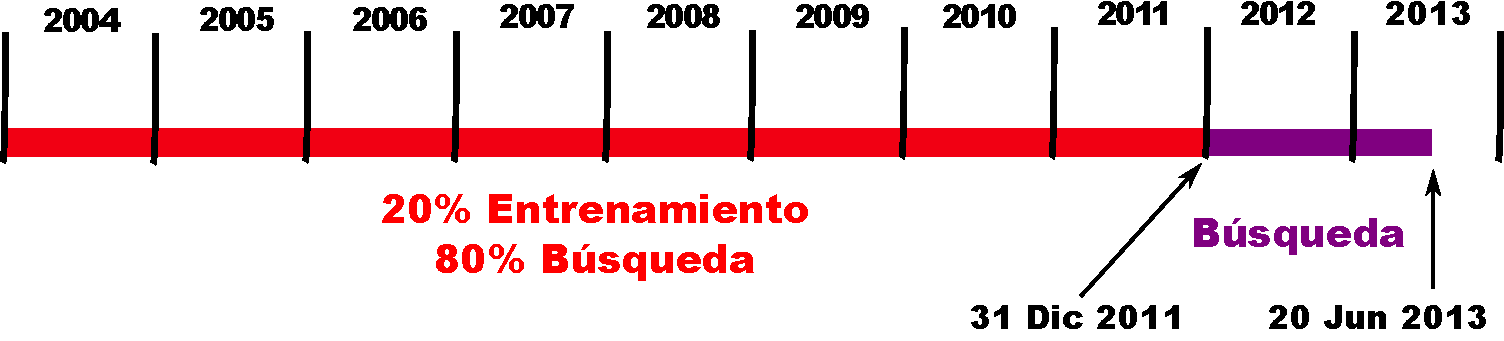
\includegraphics[width=\textwidth]{fig/seleccionAuger/periodosDGL}
	\caption{División de los datos en muestra de entrenamiento y búsqueda. Se utilizó el 20$\%$ de los datos entre el 01 Ene 2004 y el 31 Dic 2011 como muestra de entrenamiento. El resto y la totalidad entre el 1 Ene 2012 y el 20 Jun de 2013 se dejaron para búsqueda. El período equivalente de busqueda corresponde a aproximadamente a 3.2 años a detector completo.}
	\label{fig:periodosDGL}
	\end{center}
	\end{figure}
	%
	
	La elección de estas fechas, si bien parece rebuscada, se debe simplemente a que el 31 de diciembre de 2011 fue la fecha l\'imite del primer escrutinio de datos en DGL.
	Como finalizado ese periodo el análisis se mantuvo invariable, todos los datos registrados se utilizaron en la búsqueda.
	
	Con el fin de entrenar el método de Fisher para que discrimine los neutrinos de los eventos hadr\'onicos más profundos, se aplicó un requisito adicional sobre los eventos clasificados como inclinados en DGL.
	Dado que el trigger local ToT es un buen indicador de señales extendidas en el tiempo, se entrenó el método con solo con los eventos que presentaron más del $75\%$ de estaciones ToT.
	Una vez hecho esto, para definir el criterio de selección se dividió la muestra de eventos inclinados en 5 regiones según el ángulo reconstruido y en cada una de ellas se entrenó un observable de Fisher diferente.
	El conjunto de variables utilizadas en cada región se describe en la tabla \ref{tab:fisherDGL}. 
	%
	\begin{table}[h!]
		\begin{center}
		\renewcommand{\arraystretch}{1.4}
		\footnotesize
			\begin{tabular}{|l|c|c|c|c|c|}
			\hline
			& Región 1 & Región 2 & Región 3 & Región 4 & Región 5 \\
			\hline
			$\theta_{Rec}$ & $(58.5^\circ,61.5^\circ]$ & $(61.5^\circ,64.5^\circ]$ &$(64.5^\circ,67.5^\circ]$ &$(67.5^\circ,70.5^\circ]$ & $(70.5^\circ,76.5^\circ]$ \\
			\hline
			\multirow{4}{*}{$\cal{F}$}  & \multicolumn{5}{c|}{AoP$_n$} \\
			                 & \multicolumn{5}{c|}{$\prod_n$AoP$_n$} \\
			                 & \multicolumn{5}{c|}{$n$ estaciones más tempranas} \\
			                 & \multicolumn{3}{c|}{$n\leq5$} & \multicolumn{2}{c|}{$n\leq4$} \\
			\hline
			\end{tabular}
			\caption{\label{tab:fisherDGL}
			Variables utilizadas para entrenar el método de Fisher en cada una de las regiones definidas por el ángulo reconstruido. En las regiones 1 a 3 se utiliza el AoP de las 5 estaciones más tempranas de los eventos y su producto. En las regiones 4 y 5 el análogo de las primeras 4 estaciones.}
		\end{center}	 
	\end{table}
	%
	
	Las regiones 1 a 3, las menos inclinadas, requieren al menos 5 estaciones disparadas mientras que en las regiones 4 y 5 se consideró suficiente contar con 4.
	Las distribución de la variable de Fisher para cada una de estas regiones puede observarse en la figura \ref{fig:fisherDGL}.
	%
	\begin{figure}[ht]
	\begin{center}
	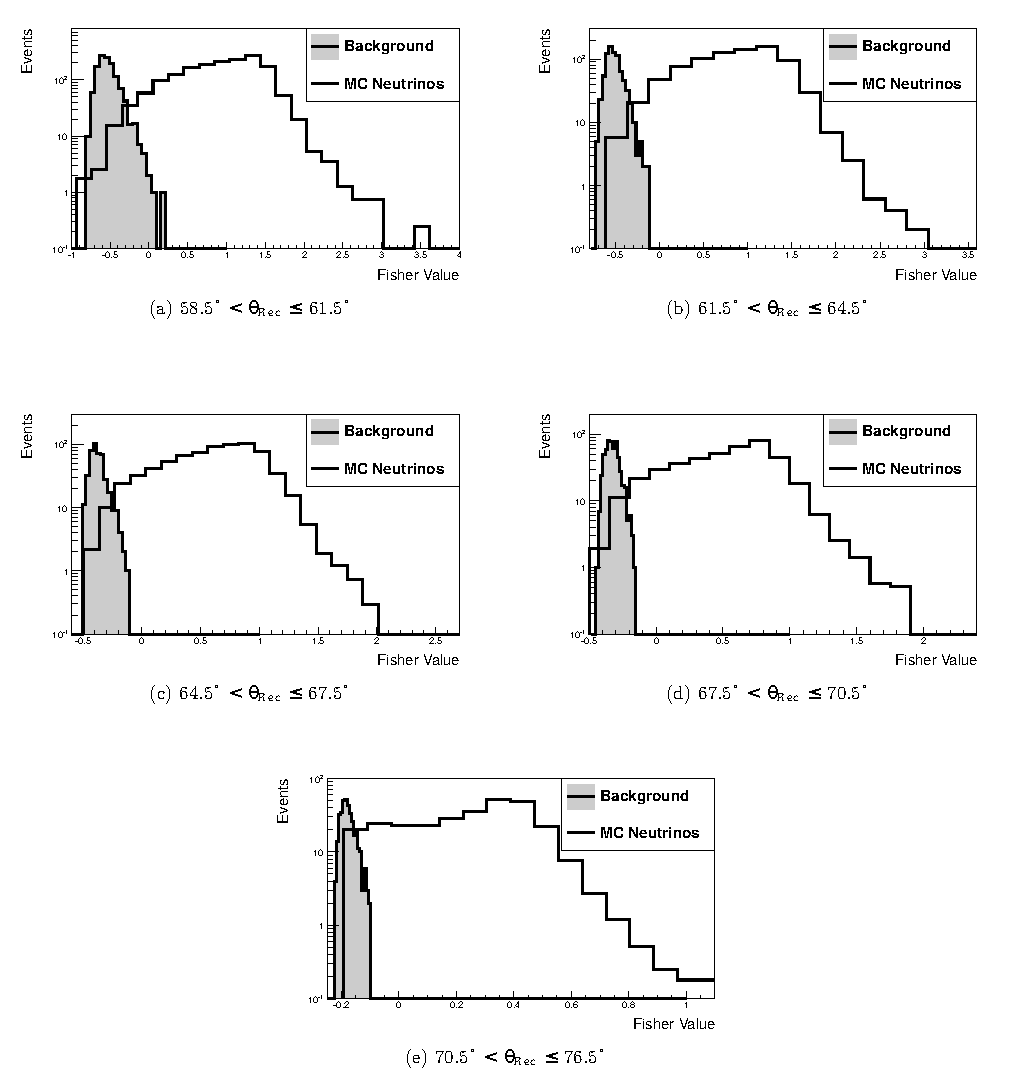
\includegraphics[width=\textwidth]{fig/seleccionAuger/fisherDGL}
	\caption{Distribuci\'on de la variable de Fisher de fondo y se\~nal para cada una de las regiones definidas en el an\'alisis DGL. Cabe destacar que la separación entre muestras crece con el ángulo reconstruido.}
	\label{fig:fisherDGL}
	\end{center}
	\end{figure}
	%
	Una vez obtenidas las variables de Fisher se ajustó la cola de las muestras de fondo, en la region de  $[1\sigma, 3\sigma]$ con el modelo exponencial, según se describió en la sección \ref{sbsc:fondo}.
	Luego se utilizaron las regiones de $[3\sigma, 6\sigma]$ para validar el modelo.
	La tabla \ref{tab:predDGL} muestra la cantidad de eventos observados y predichos por el modelo en cada una de las regiones.
	%
	\begin{table}[h!]
	\begin{center}
		\renewcommand{\arraystretch}{1.4}
		\footnotesize
	 \begin{tabular}{|c|c|c|c|c|c|}
	 \hline
	 & \multicolumn{5}{c|}{Observado - Predicho} \\
	 & Región 1 & Región 2 & Región 3 & Región 4 & Región 5 \\
	 \hline
	 $[3\sigma, 4\sigma]$ & 4 - 5.7 &2 - 3.5 & 1 - 3.7 & 0 3.5 & 0 - 3.7 \\
	 $[4\sigma, 5\sigma]$ & 1 - 1.9 & 0 - 1.3 & 0 - 1.4 & 0 - 1.1 & 0 - 1.5 \\
	 $[5\sigma, 6\sigma]$ & 0 - 0.6 & 0 - 0.3 & 0 - 0.5 & 0 - 0.5 & 0 - 0.6 \\
	 \hline
	 \end{tabular}
	 \caption{Cantidad de eventos observados y predichos por el modelo exponencial para las distincias regiones definidas por el ángulo reconstruido. Se observa buen acuerdo o sobreestimación de parte del modelo. Esto quiere decir que el corte obtenido será seguro.}
	 \label{tab:predDGL}
	\end{center}
	\end{table}
	Dado que la predicción del modelo se encuentra en acuerdo o sobreestima lo observado, se considera que el corte obtenido mediante este método sobreestimará la contaminación, dejando el análisis del lado ``seguro''.
	
	En el panel superior de la figura \ref{fig:fisher2dDGL} se muestran las distribuciones bidimensionales de la variable de Fisher y el ángulo reconstruido para las muestras de entrenamiento y señal. En linea llena se grafican los cortes obtenidos en cada una de las variables de Fisher dividias segun la región definida por el ángulo reconstruido.
	Para fijar estos cortes, se consideró que un evento de contaminación en todas las regiones (0.2 por región) cada 20 años constituía un nivel aceptable.
	Finalmente, en lugar de un corte en la variable de Fisher par acada región, se utilizó la interpolación lineal obtenida entre distintas regiones, lo que se muestra en el panel inferior de la figura \ref{fig:fisher2dDGL}.
	%
	\begin{figure}[ht]
	\begin{center}
	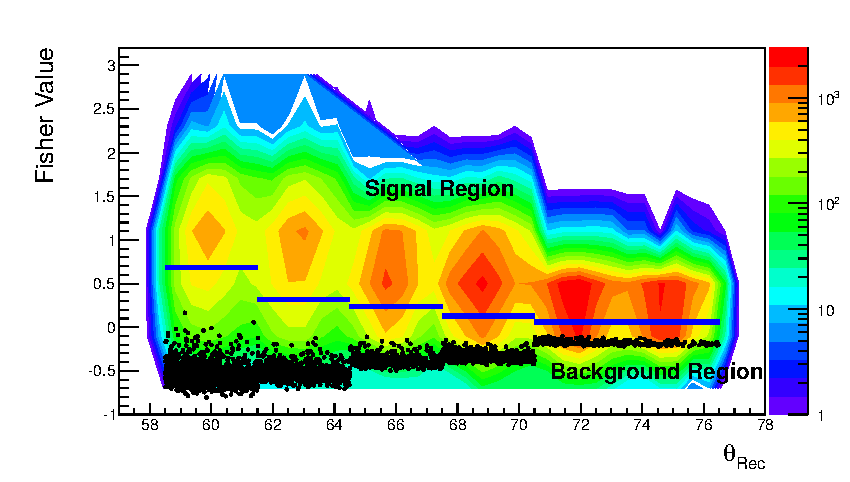
\includegraphics[width=0.7\textwidth]{fig/seleccionAuger/fisher2dDGL}\\
	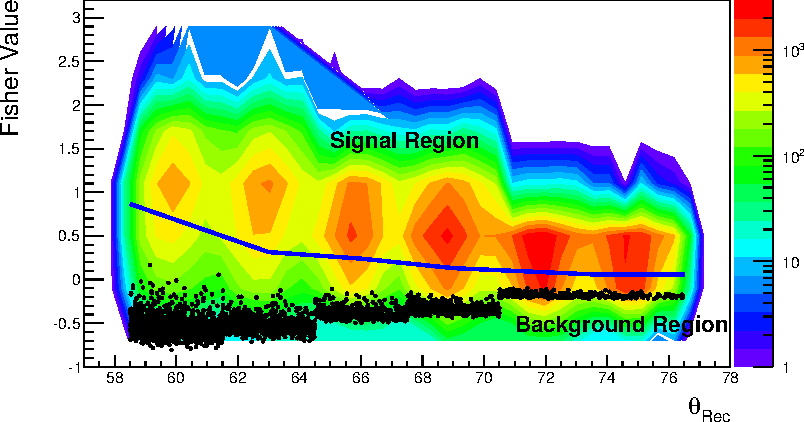
\includegraphics[width=0.7\textwidth]{fig/seleccionAuger/fisher2dInterpolDGL}
	\caption{Distribución de la variable de Fisher como función del ángulo reconstruido. La muestra de neutrinos MC se muestra en colores mientras que la de fondo (datos) es representada con puntos. Arriba: En linea llena se señalan los cortes en la variable de Fisher obtenidos para cada región. Abajo: En linea llena se muestra el corte efectivo obtenido mediante interpolación lineal.}
	\label{fig:fisher2dDGL}
	\end{center}
	\end{figure}
	%
	\clearpage
	
	\subsection{Identificación de neutrinos DGH}
	
	En el caso de la busqueda de neutrinos DGH se utilizó como muestra de entrenamiento datos que ya habian sido utilizados en la primer búsqueda de neutrinos ES, que incluyó hasta el 31 de octubre de 2007\footnote{La muestra de eventos inclinados seleccionada por ES esta contenida casi completamente en la de DGH, lo que invalida realizar una nueva b\'usqueda sobre la misma.}.
	%
	\begin{figure}[ht]
	\begin{center}
	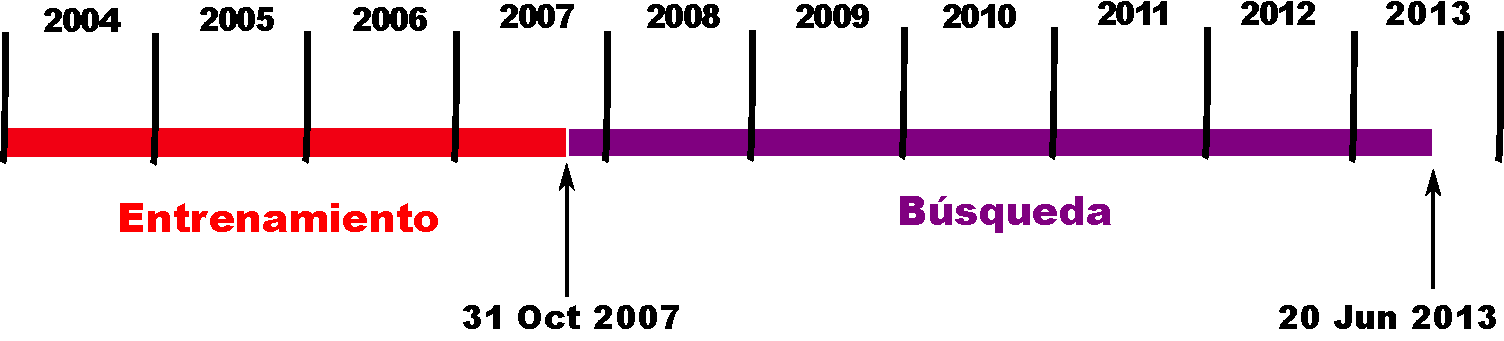
\includegraphics[width=\textwidth]{fig/seleccionAuger/periodosDGH}
	\caption{División de los datos en muestra de entrenamiento y búsqueda. Para el análisis de DGH se utilizaron los datos desde el 01 Ene 2004 hasta el 31 Oct 2007 como muestra de entrenamiento, mientras que desde el 1 Nov 2007 hasta el 20 Jun 2013 fueron utilizados para búsqueda.}
	\label{fig:periodosDGH}
	\end{center}
	\end{figure}
	%
	Dado que la selección de eventos inclinados de los análisis DGH y ES comparte una gran fracción de los datos, no habría sido lícito utilizar una muestra ya analizada para una nueva búsqueda.
	Por ende, el escrutinio de candidatos se realizó sobre los eventos registrados desde el 1 de noviembre 2007 hasta el 20 de junio de 2013.
	Este período corresponde aproximadamente a 4 años de detector completo.
	
	A diferencia del análisis de DGL, en DGH se dividió las muestras de entrenamiento no por el ángulo reconstruido sino según el tamaño de los eventos.
	La tabla \ref{tab:fisherDGH} muestra la división y las variables utilizadas para entrenar el método.
	%
	\begin{table}[h!]
		\begin{center}
		\renewcommand{\arraystretch}{1.4}
		\footnotesize
			\begin{tabular}{|l|c|c|c|}
			\hline
			Multiplicidad\hfill$\rightarrow$& Baja & Media & Alta \\
			\hline
			$N_{St}$\hfill$\rightarrow$ & $[4,6]$ & $[7,11]$ & $[12,\infty)$ \\
			\hline
			\multirow{4}{*}{$\cal{F}$\hspace*{25mm}$\rightarrow$}  & \multicolumn{3}{c|}{AoP$_n$} \\
			                 & \multicolumn{3}{c|}{AoP$^2_n$} \\
			                 & \multicolumn{3}{c|}{$\prod_n$AoP$_n$} \\
			                 & \multicolumn{3}{c|}{Parámetro de asimetría} \\
			\hline
			\end{tabular}
			\caption{\label{tab:fisherDGH}
			Variables utilizadas para entrenar el método de Fisher en cada una de las multiplicidades, definidas por el número de estaciones del evento.}
		\end{center}	 
	\end{table}
	%
	Según el tamaño del evento se definieron tres \emph{multiplicidades}, de 4 a 6 estaciones, de 7 a 11 y de más de 12.
	Al igual que en el análisis de DGL, se consideró que estas submuestras presentan diferencias físicas lo suficientemente importantes como para poder ser separadas por el mismo clasificador.
	El resultado del entrenamiento se muestra en la figura \ref{fig:fisherDGH}, donde se grafica la variable de Fisher para cada una de las multiplicidades.
	%
	\begin{figure*}
	\begin{center}
	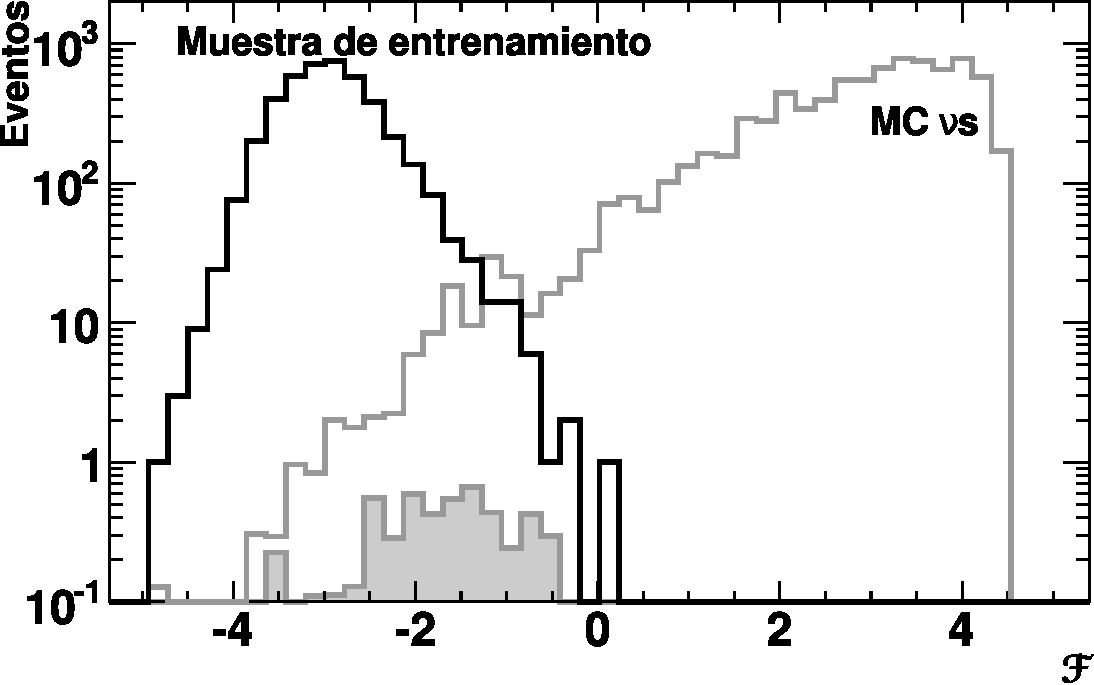
\includegraphics [width=0.47\textwidth]{fig/seleccionAuger/fishDist_altos_1.pdf}\hfill
	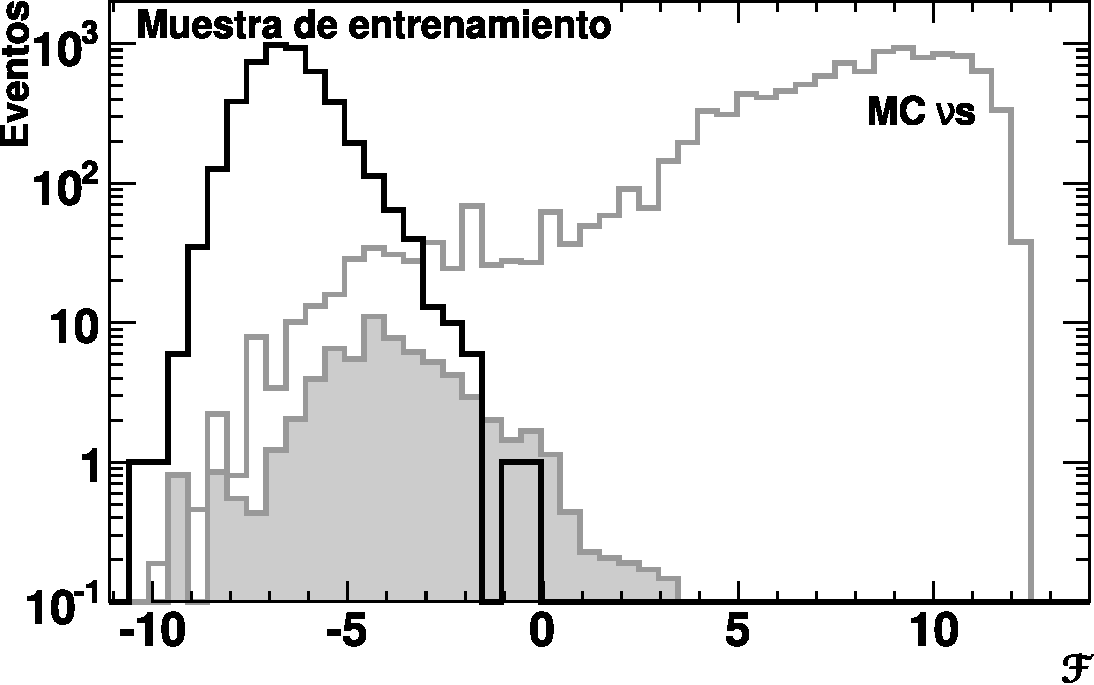
\includegraphics [width=0.47\textwidth]{fig/seleccionAuger/fishDist_altos_2.pdf}\\
	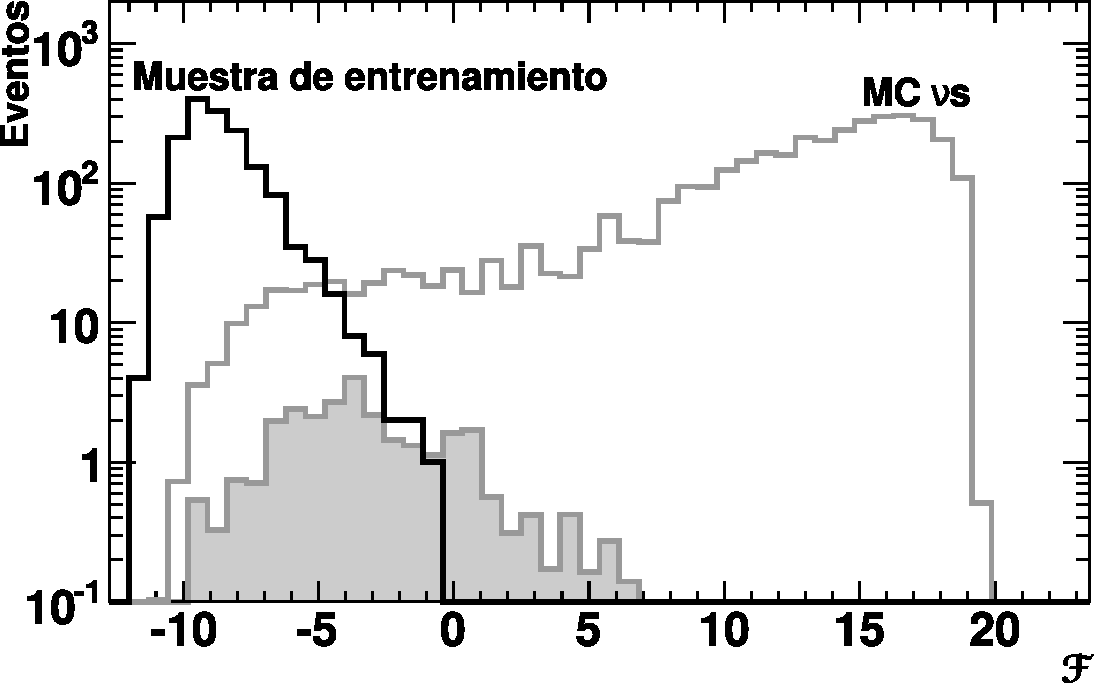
\includegraphics [width=0.47\textwidth]{fig/seleccionAuger/fishDist_altos_3.pdf}
	\end{center}
	\caption{
	Distribuciones del discriminante de Fisher~($\cal{F}$) de las muestras background (datos del 1 de enero de 2004 al 31 de octubre de 2007) y señal (MC de neutrinos) para los tres grupos de multiplicidad: eventos pequeños (\textit{arriba}), medianos (\textit{medio}) y grandes (\textit{abajo}). Se muestra sombreado la distribución de los eventos MC cuyo punto de primera interacción ocurre alto en la atmósfera (aunque, en general, a mayor profundidad que la que se espera para lluvias hadrónicas).
	}
	\label{fig:fisherDGH}
	\end{figure*}
	%
	En particular, el histograma sombreado resalta los eventos provenientes de neutrinos que interactuaron alto en la atmósfera.
	Estos en general generaron valores en la variable de Fisher bajos, similar al exhibido por los eventos de la muestra de fondo (iniciados alto en la atmósfera), aunque un poco mayor.
	Este hecho sirve de alguna manera como confirmación de que el clasificador se comporta de manera adecuada. 
	Analogamente, si hubiera algun evento con características de neutrino profundo en la muestra de entrenamiento, habría obtenido un valor alto en la variable de Fisher.
	
	Al igual que en DGL, una vez obtenidas la variables de Fisher se procedió a obtener el valor del corte que definirá el criterio de selección.
	Para ello se utilizó el procedimiento expuesto en la sección \ref{sbsc:fondo} pidiendo un evento de contaminación en las tres multiplicidades cada 20 años.
	En el panel izquierdo de la figura \ref{fig:fisherZoom} pueden observarse los ajustes exponenciales sobre las colas de las muestras de fondo junto con las predicciones realizadas sobre las zonas de  $[3\sigma, 6\sigma]$. 
	La cantidad de eventos de la muestra de entrenamiento en cada una de las zonas esta de acuerdo con la predicción dada por el modelo exponencial.
	%
	\begin{figure*}
	\begin{center}$
	\begin{array}{cc}
	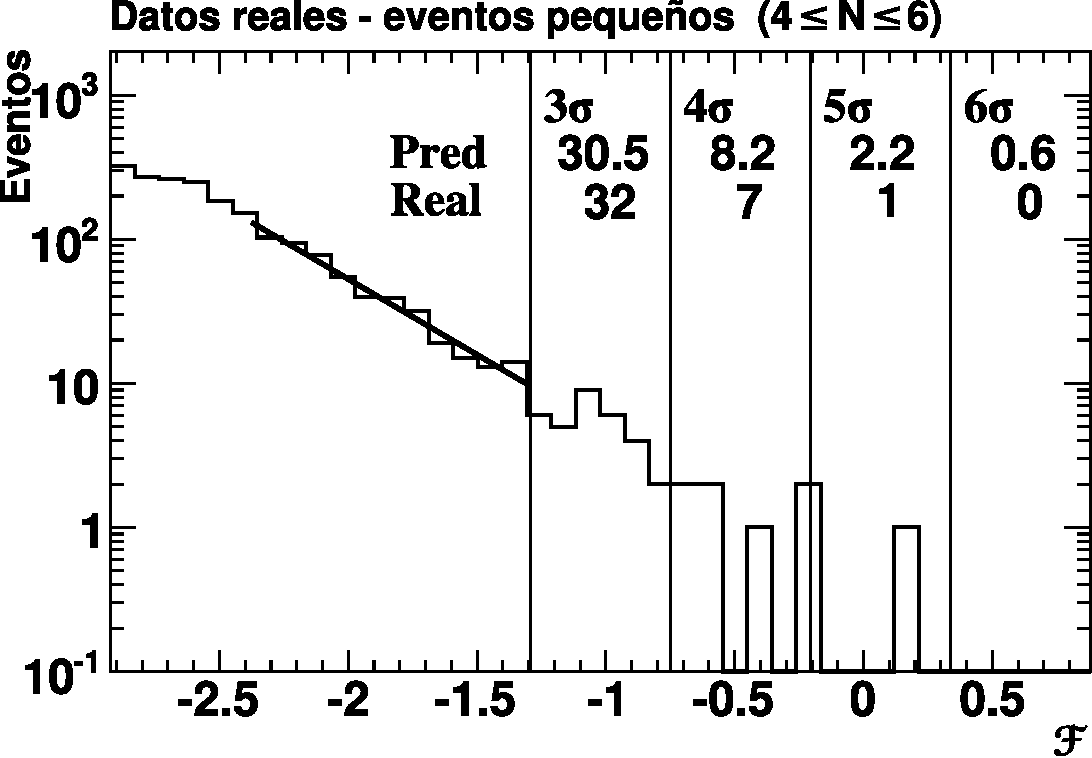
\includegraphics [width=0.47\textwidth]{fig/seleccionAuger/fisherZoom1.pdf} &
	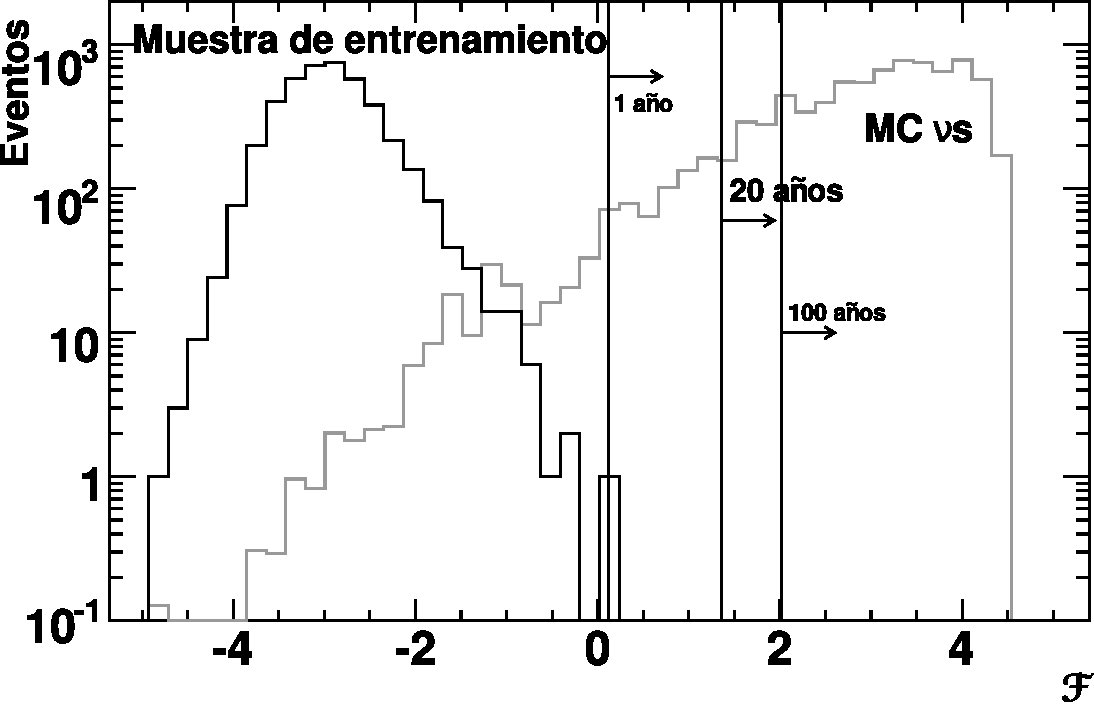
\includegraphics [width=0.47\textwidth]{fig/seleccionAuger/fishDist_cuts_1.pdf} \\
	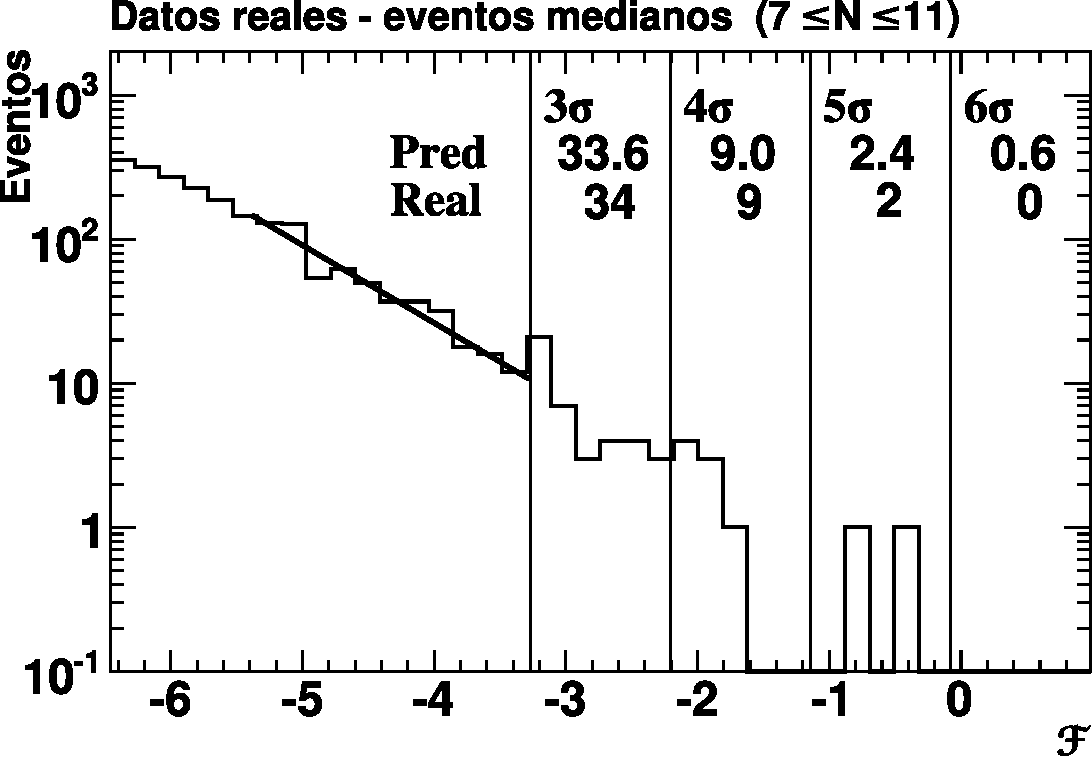
\includegraphics [width=0.47\textwidth]{fig/seleccionAuger/fisherZoom2.pdf} &
	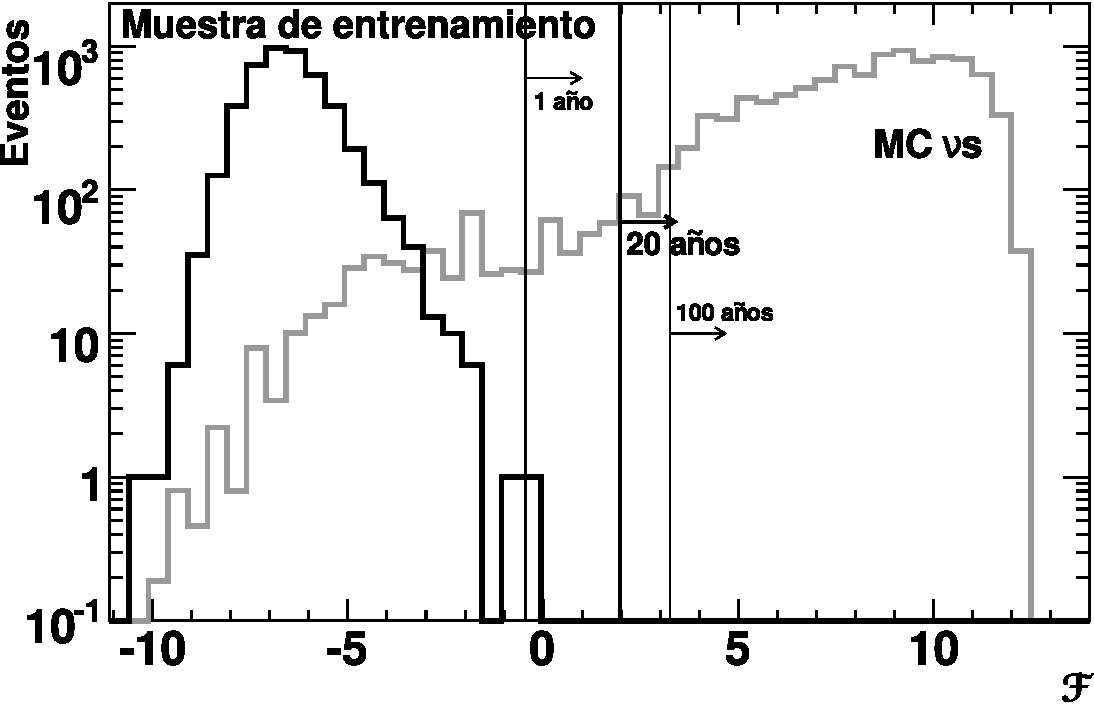
\includegraphics [width=0.47\textwidth]{fig/seleccionAuger/fishDist_cuts_2.pdf} \\
	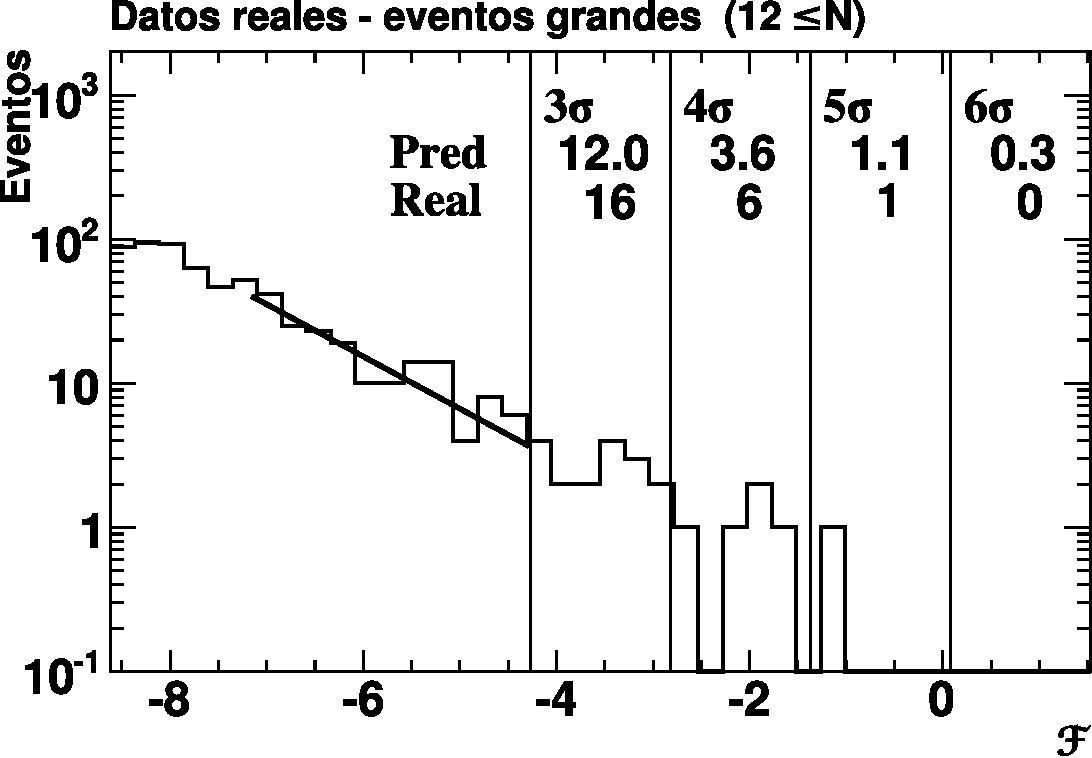
\includegraphics [width=0.47\textwidth]{fig/seleccionAuger/fisherZoom3.pdf} &
	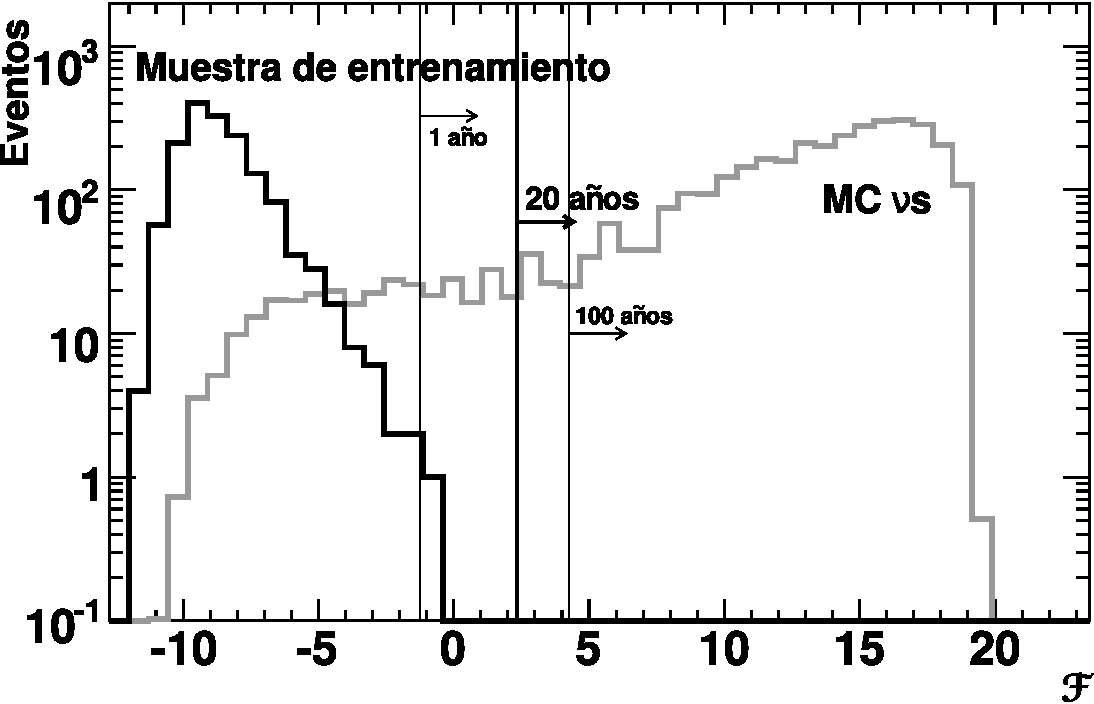
\includegraphics [width=0.47\textwidth]{fig/seleccionAuger/fishDist_cuts_3.pdf} 
	\end{array}$
	\end{center}
	%\vskip -0.7cm
	\caption{
	\textit{\textit{columna izquierda}}: ajuste exponencial sobre el intervalo $[1\sigma,3\sigma]$ de la cola de la distribución de Fisher~${\cal F}$ para la muestra de entrenamiento. Se indica también el número de eventos predicho (Pred.) y medido (Real) para cada una de las zonas de prueba ($[3\sigma,4\sigma]$, $[4\sigma,5\sigma]$, $[5\sigma,6\sigma]$ y $[6\sigma,7\sigma]$). \textit{derecha}: distribuciones del discriminante de Fisher~($\cal{F}$) de las muestras background (datos del 1-ene-04 al 31-oct-07) y señal (MC de neutrinos) para los tres grupos de multiplicidad: eventos pequeños (\textit{arriba}), medianos (\textit{mitad}) y grandes (\textit{abajo}). Las líneas verticales indican el corte en el valor del discriminante de Fisher correspondientes a un evento de background cada 1, 20 y 100 años.
	}
	\label{fig:fisherZoom}
	\end{figure*}
	
	\subsection{Identificación de neutrinos ES}
	
	Hasta la fecha, en Auger hubo dos criterios de identificación de neutrinos ES que estuvieron vigentes en períodos de tiempo diferentes. 
	La fecha de inflexión entre los dos análisis fue el 31 May 2010.
	A partir de aquí se identificará al primer análisis como el \emph{original}, mientras que el segundo será el análisis \emph{nuevo}.
	El primero utilizó como muestra de entrenamiento los primeros dos meses de datos de 2004 y el resto del período de vigencia como muestra de búsqueda, hasta el 31 de mayo de 2010.
	Por las mismas razones que en DGH, los datos que ya hab\'ian sido utilizados en esta búsqueda sirvieron de muestra de entrenamiento para el nuevo análisis, que busc\'o candidatos hasta el 20 de junio de 2013.
	Esta situación se describe en la figura \ref{fig:periodosES}.
	%
	\begin{figure}[ht]
	\begin{center}
	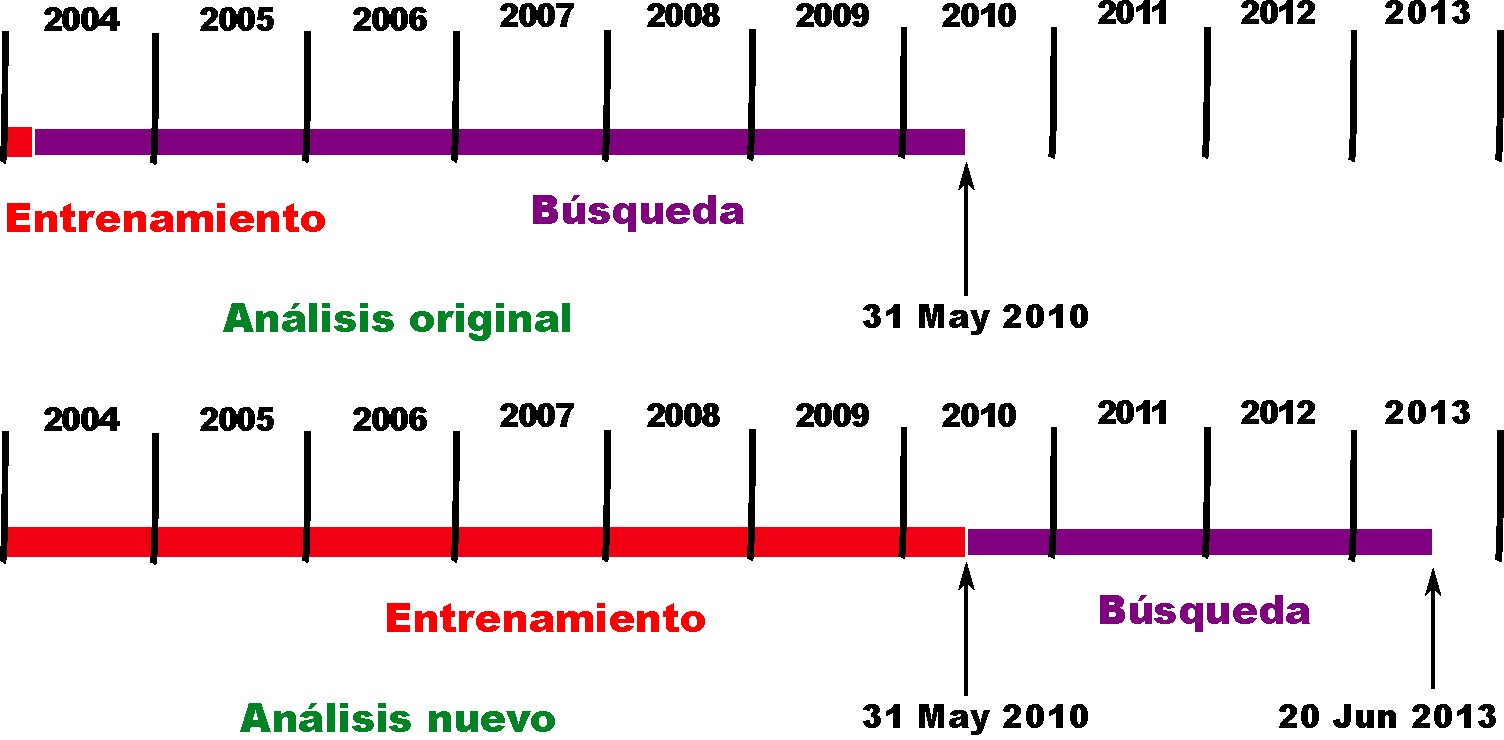
\includegraphics[width=\textwidth]{fig/seleccionAuger/periodosES}
	\caption{División de los datos en muestra de entrenamiento y búsqueda para el análisis de ES.
	El panel superior muestra la división para el análisis original, mientras que el inferior para el nuevo.
	En el primer análisis solo se utilizaron dos meses de datos de 2004 como muestra de entrenamiento, y se buscaron neutrinos en los datos hasta el 31 May 2010.
	El nuevo análisis empleó todos los datos utilizados hasta el momento como muestra de entrenamiento, y llevó a cabo la busqueda en el período 1 Jun 2010 a 20 Jun 2013.}
	\label{fig:periodosES}
	\end{center}
	\end{figure}
	%
	
	\subsubsection{Análisis original}
	
	La selección de luvias jóvenes del análisis original fue llevada a cabo utilizando cortes cuadrados duros.
	Las variables utilizadas y los cortes aplicados se detallan a continuación.
	\begin{itemize}
	 \item Se aplicó un corte sobre la fracción de estaciones ToT: ToTF$>0.6$
	 \item Se utilizó un corte sobre la cantidad de estaciones de estaciones con trigger ToT y AoP$>1.4$: ${\tt nOfflineToT}\geq3$
	 \item Se requirió además que el evento sea clasificado como \texttt{IsT4Nu}. Esta etiqueta señala eventos inclinados e iniciados de manera profunda al pedir al menos 3 estaciones con AoP$>1.4$ y velocidades entre cada una de ellas cumpla $0.285{\rm \frac{m}{ns}}<V_{ij}<0.31{\rm \frac{m}{ns}}$
	\end{itemize}

	La figura \ref{fig:totFES} muestra la distribución de ToTF antes y despues de aplicar los cortes sobre \texttt{nOfflineToT} e \texttt{IsT4Nu}.
	La muestra de datos corresponde a 1 Ene 2004 - 31 Oct 2007. Por otro aldo, en ambos casos la muestra de señal se normalizó al histograma de datos.
	%
	\begin{figure}[ht]
	\begin{center}
	\includegraphics[width=0.47\textwidth]{fig/seleccionAuger/ToTF_forThesis}\hfill
	\includegraphics[width=0.47\textwidth]{fig/seleccionAuger/ToTF_with_noToT_and_hasTriangle_forThesis}
	\caption{Distribución de la variable ToTF para datos entre 1 Ene 2004 y 31 Oct 2007 y para la muestra de neutrinos ES. El panel izquierdo corresponde a haber aplicado los criterios de calidad y de clasificación de lluvias inclinadas, mientras que el panel derecho se grafican las distribuciones luego de aplicar los cortes en \texttt{nOfflineToT} e \texttt{IsT4Nu}. En ambos casos la muestra de neutrinos se normalizó a la de datos.}
	\label{fig:totFES}
	\end{center}
	\end{figure}
	%
	
	Si bien es posible deducir que la eficiencia de detección es bastante alta (ronda el $85\%$ respecto del nivel de trigger), ninguna de las distribuciones de datos permitiría realizar alguna estimación de la contaminación.
	Por este motivo surgió la necesidad de pensar en un nuevo criterio de identificación de lluvias jóvenes para la búsqueda de neutrinos ES.
	
	\subsubsection{Análisis nuevo}
	
	La razón principal para implementar un nuevo análisis para detectar neutrinos ES fue lograr una estimación de la contaminación en la selección.
	El objetivo fue buscar variables que permitan realizar el procedimiento descripto en la sección \ref{sbsc:fondo}, manteniendo un valor en la eficiencia de identificación similar al alcanzado en el análisis original.
	
	Como se mostró en la figura \ref{fig:aop_vs_NStation} el valor de AoP en la muestra de MC ES es en promedio mayor que para los datos.
	Adem\'as, a diferencia de los eventos DG los ES no presentan ninguna asimetría considerable entre la parte temprana y tardía de la lluvia.
	Luego de varias iteraciones del método esquematizado en la figura \ref{fig:entrenamiento}, aplicando el método de Fisher a decenas de variables, ninguna mostr\'o un desempe\~no sustancialmente mayor al alcanzado por la variable AoP promedio (\aop{}), por lo que se la utiliz\'o como \'unica variable discriminante.
	
	Para evitar falsos candidatos se decidió excluir del promedio ciertas estaciones propensas a presentar valores de \aop{} artificialmente elevado\footnote{Estas estaciones sí fueron utilizadas en el cálculo de las variables sensibles a la inclinación debido a que los tiempos de inicio de la señal usualmente son correctos.}, a saber:
	\begin{itemize}
	 \item Estaciones con PMT's cuyo dínodo se encuentra saturado: estas estaciones presentan el valor del pico de la señal disminuido, por lo que poseen un valor de AoP por encima del valor real.
	 \item Estaciones con trigger local T1: al ser pequeña, la señal es propensa a introducir ruido en el promedio \aop{}.
	 \item Estaciones con dobles picos no descartadas en por el algoritmo de limpieza de traza.
	\end{itemize}
	
	El algoritmo de limpieza de traza tiene como objetivo eliminar las estaciones en las que el tiempo de disparo no sea claro. 
	Cuando en la FADC existe una sección espúrea que no se encuentra lo suficientemente separada de la traza real como para inducir un valor de tiempo de disparo artifical, usualmente no es descartada.
	Como la precencia de estos picos múltiples provocan un aumento espúreo del valor de \aop{} es clave descartar estas estaciones, especialmente si el evento tiene multiplicidad baja.
	
	Un ejemplo de este tipo de eventos se muestra en la figura \ref{fig:doublePeakEvent}.
	De las 4 estaciones con trigger T2, la 882 presenta un valor de AoP=1.92, por encima del promedio para este tipo de eventos ($\sim1.4$). 
	El panel derecho de la figura muestra la traza de la estación, en la que claramente se distinguen dos picos generados por muones muy cercanos en tiempo.
	%
	\begin{figure}[ht]
	\begin{center}
	\includegraphics[height=0.35\textwidth]{fig/seleccionAuger/2629688_nice}
	\hfill
	\includegraphics[height=0.35\textwidth]{fig/seleccionAuger/ev2629688_pmtAvg_anode}
	\caption{Evento 2629688. Izquierda: huella del evento. Los circulos negros señalan las 4 estaciones con T2, mientras que los grises las que poseen T1. Derecha: señal calibrada y promediada sobre los tres PMT's de la estación 882. Esta presenta una clara estructura de doble pico. }
	\label{fig:doublePeakEvent}
	\end{center}
	\end{figure}
	%
	
	Para salvar este inconveniente se aplicó el algoritmo que se detalla en el ap\'endice \ref{ap:doublePeakDet}.
	Es importante destacar que las trazas de las simulaciones de neutrinos ES no presentan este tipo de estructura de doble pico, sino señales con picos pequeños y de corta duración (típica señal electromagnética como la de la figura \ref{fig:t2_tot}).
	Tal es así que este algoritmo sólo rechaza al rededor del $1\%$ de las estaciones de los eventos ES, aunque el AoP promedio por estación es aproximadamente 3.3.
	La pérdida pesada de eventos MC debida a este requerimento es de al rededor de $1.2\%$ ($\sim 0.7\%$ sin peso).
	
	Una vez removidas las estaciones que podrían aumentar artificialmente el valor de \aop{}, se realizó el ajuste exponencial y se analizaron las predicciones en las zonas de prueba, como se muestra en la figura \ref{fig:fitExpoES}.
	%
	\begin{figure}[ht]
	\begin{center}
	\includegraphics[width=0.7\textwidth]{fig/seleccionAuger/fitExponential_test_with3st_forThesis}
	\caption{Arriba: Ajuste exponencial de la cola de la distribución de entrenamiento y predicciones en las zonas de prueba ($[3\sigma,4\sigma]$, $[4\sigma,5\sigma]$, $[5\sigma,6\sigma]$ y $[6\sigma,7\sigma]$). El corte obtenido es \aop{}$>1.83$.}
	\label{fig:fitExpoES}
	\end{center}
	\end{figure}
	%
	Al igual que en los análisis de DG, lo predicho por el modelo se encuentra por encima de lo observado, siendo el corte seguro.
	
	Como se expuso en la sección \ref{sbsc:3StIncl}, se debe tener especial cuidado con los eventos de 3 estaciones, por ende requieren un trato diferencial.
	Estos, son m\'as propensos a ser clasificados como candidatos a neutrinos debido a que una fluctuación en el AoP en solo una de sus estaciones puede inducir un cambio en \aop{} lo suficientemente grande como para pasar el corte de selección.
	Para asegurarse de que un valor elevado en \aop{} no proviene de una fluctuación en una de sus estaciones, se exige que el mínimo AoP de los eventos de 3 estaciones (\aopmin{}) sea al menos 1.4.
	Este valor esta basado en el elegido en el análisis original para seleccionar estaciones con trazas extendidas en el tiempo.
	La figura \ref{fig:minAoP} muestra la distribución de esta variable para los eventos de 3 estaciones de las muestras de señal y fondo, antes de aplicar el corte en \aop{}.
	%
	\begin{figure}[ht]
	\begin{center}
	\includegraphics[width=0.7\textwidth]{fig/seleccionAuger/minAoP_forThesis}
	\caption{Distribución de \aopmin{} para eventos de 3 estaciones antes de aplicar el corte en \aop{}. El corte ${\rm AoP_{min}}>1.4$ se muestra en línea punteada.}
	\label{fig:minAoP}
	\end{center}
	\end{figure}
	%
	Este corte reduce la eficiencia total en $1.3\%$ ($8\%$ para eventos de 3 estaciones).
	
% 	\begin{sidewaystable}[ht!]
% 	\begin{center}
% 		\renewcommand{\arraystretch}{1.4}
% 		\footnotesize
% 		\begin{tabular}{l|c|c|c}
% 		\hline
% 		Búsqueda & Earth-skimming (ES)           & Downward-going                        & Downward-going                       \\
% 				&                               & {\it high} angle (DGH)                & {\it low} angle (DGL)                \\
% 		\hline 
% 		Sabores e interacciones & $\nu_\tau$ CC & $\nu_e,~\nu_\mu~,\nu_\tau$ CC $\&$ NC &  $\nu_e,~\nu_\mu~,\nu_\tau$ CC $\&$ NC \\
% 
% 		Rango angular & $\theta>90^\circ$             & $\theta \in (75^\circ, 90^\circ)$ & $\theta \in (60^\circ, 75^\circ)$ \\
% 
% 		N$^\circ$ de estaciones(Nst) & Nst $\geq$ 3   & Nst $\geq$ 4 & Nst $\geq$ 4 \\
% 		\hline 
% 					& $-$                             & $\theta_{\rm rec}>$ 75$^{\circ}$   &   $\theta_{\rm rec}\in (58.5^\circ,~76.5^{\circ})$\\
% 		Lluvias    & $L/W > 5$                                         & $L/W > 3$ & $-$ \\
% 		Inclinadas & $\langle V\rangle\in (0.29,~0.31)~{\rm m~ns^{-1}}$ & $\langle V \rangle~<~0.313~{\rm m~ns^{-1}}$ & $-$ \\
% 				& RMS($V$)$~<~0.08~{\rm m~ns^{-1}}$                 & RMS($V$)/$\langle V\rangle<0.08$ & $-$ \\
% 		\hline 
% 				& Datos: 1 January 04 - 31 May 10 &                                     & $\geq 75\%$ de estaciones cercanas al   \\
% 				& $\geq 60\%$ of stations with  &                                      & core con ToT trigger       \\
% 		Lluvias     & ToT trigger \& AoP $>$ 1.4    & Discriminante de Fisher basado &                          \&        \\
% 		%\cline{2-2}
% 		Jóvenes   & Datos: 1 Junio 10 - 20 Junio 13   & en AoP estaciones {\it early}   & Discriminante de Fisher basado  \\
% 				& $\langle {\rm AoP} \rangle> 1.83$  &                                 & en AoP de las estaciones {\it early} \\
% 				& AoP$_{\rm min}$ $>$ 1.4 if Nst=3   &                                 & cercanas al core \\
% 		\hline
% 		\end{tabular}
% 		\vskip -3mm
% 		\caption{Resumen de los observables y valores numéricos de los cortes aplicados para seleccionar lluvias inclinadas y jóvenes en las tres búsquedas de neutrinos.} 
% 	\end{center}
% 
% 	\label{tab:cuts}
% 	\end{sidewaystable}